\documentclass[
  final,
  pagePreset=largepage,% 6in x 9in
  babelLanguage=portuguese,
  %webversion,
]{anecdote}

\usepackage{local}

%% Details of the book
%% ===================

\title{Folhas da Árvore Bodhi}
\subtitle{}
\author{}
\publisher{Publicações Sumedhārāma}
\date{2016-04-02}
% TODO: confirm edition info
\editionInfo{\textit{Primeira edição}, 2000 cópias, impressas na Malásia, 2017}
\ISBN{000-0-000000-00-0}

%% === Load further packages ===

%% === Hyphenation exceptions and corrections ===

% \hyphenation{}

\begin{document}

\ifwebversion
\webcover{%
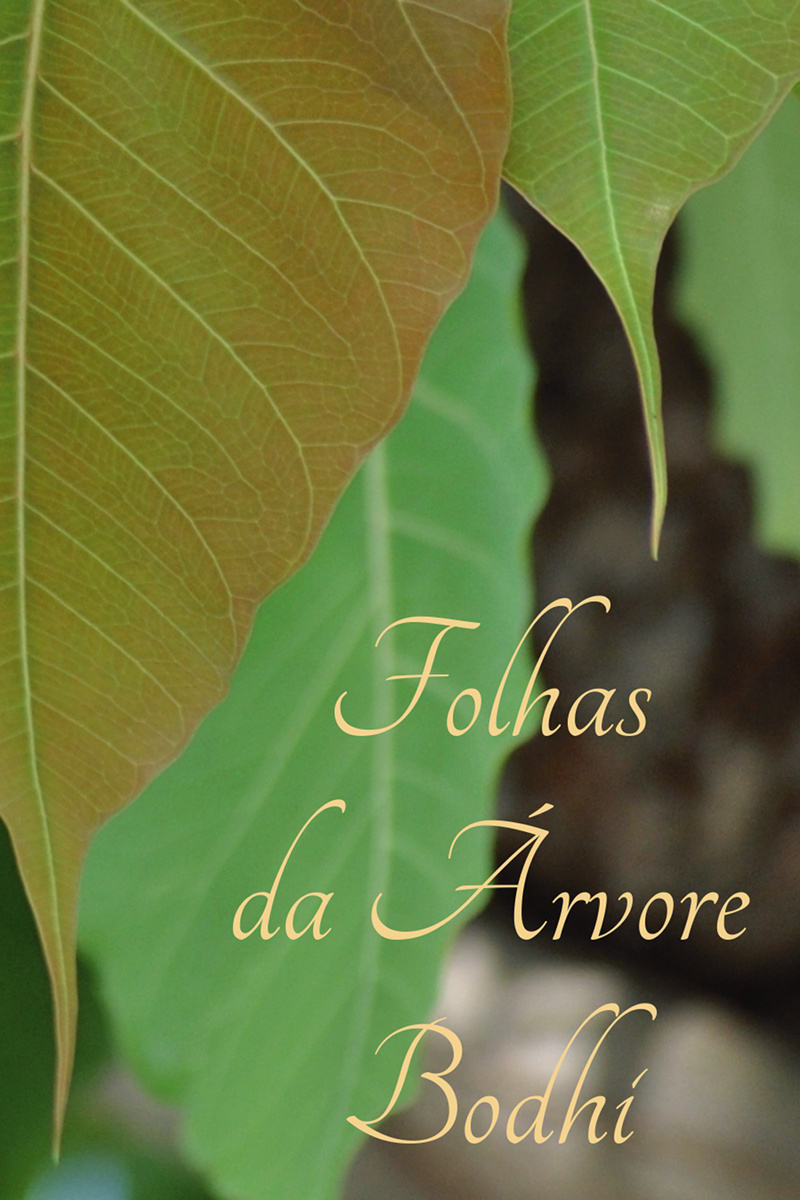
\includegraphics[height=\paperheight]{./webcover.jpg}%
}
\fi

\frontmatter

\cleartoverso
\thispagestyle{empty}

{\copyrightsize
\centering
\setlength{\parindent}{0pt}%
\setlength{\parskip}{0.8\baselineskip}%

\thetitle

Publicações Sumedhārāma\\
\href{http://sumedharama.pt}{www.sumedharama.pt}

Para distribuição gratuita\\
\textit{Sabbadānaṃ dhammadānaṃ jinati}\\
‘A oferta de Dhamma é superior a qualquer outra oferta.’

Este livro encontra-se disponível para distribuição gratuita em\\
\href{http://fsbooks.org/}{www.fsbooks.org}

ISBN \theISBN

Copyright \copyright\ Publicações Sumedhārāma 2017

Este trabalho está licenciado com uma Licença Creative Commons\\
Atribuição-NãoComercial-SemDerivações 4.0 Internacional.

Veja página \pageref{copyright-details} para mais detalhes sobre direitos e restrições desta licença.

\theEditionInfo

Editor: Appamādo Bhikkhu\\
Formatação: Venerável Gambhīro

Produzido com o sistema tipográfico \LaTeX.\\
Fonte utilizada: Gentium, Glacial~Indifference, Crimson~Roman,\\
Alegreya~Sans e Fira~Sans.

}


\chapterstyle{high-left-arvore}

\cleartorecto
\tableofcontents*

\chapterstyle{high-arvore}

% Nota de Edição
\chapter{Nota de Edição}

No decorrer do processo do estabelecimento do Budismo Theravada da
Floresta em Portugal, foram traduzidos para Português várias palestras e
artigos, de monges e monjas desta Tradição,

Este livro é uma compilação desses textos que foram escolhidos e
traduzidos com o intuito de levar o Dhamma, versado pelos monásticos
Theravada, aos países lusófonos, de forma a que estes possam beneficiar
e melhor compreender o ensinamento do Buddha. A maior parte destes
textos são transcrições de palestras, à excepção de: 'A Perspectiva da
Floresta', extraído do livro 'Small Boat, Great Mountain', de Ajahn
Amaro, e 'Emoções Maduras', artigo escrito por Ajahn Vajiro para a
Newsletter do Mosteiro Bodhinyanarama.

Todos os autores destes textos são monásticos seniores da tradição de
Ajahn Chah.

Que o ensinamento aqui expresso possa contribuir para a
consciencialização e libertação de todos os seres.


\addtocontents{toc}{\protect\enlargethispage{2\protect\baselineskip}}

\cleartorecto
\thispagestyle{empty}
\vspace*{5em}
\newlength\titleLength
\newlength\xheight

{\centering

\settowidth{\titleLength}{%
  {\Large\chapterTitleFont\scshape\MakeLowercase{\thetitle}}%
}

{\Large\chapterTitleFont\scshape\MakeLowercase{\thetitle}}\\[0.3\baselineskip]
\setlength{\xheight}{\heightof{X}}
\raisebox{0.5\xheight}{\color[gray]{0.4}\rule{\titleLength}{0.1pt}}\\[0.3\baselineskip]
{\itshape
\thesubtitle}

}




\mainmatter

% Samma Samādhi
\chapterAuthor{Ajahn Chah}
\chapter{Samma Samādhi}
\tocChapterNote{Ajahn Chah}

\section{Desapego dentro da prática}

Observemos o exemplo do Buddha. Ele era exemplar quer, na sua própria
prática quer, nos métodos que usou para ensinar os discípulos. O Buddha
ensinou as bases da prática como métodos para que nos livremos do
orgulho. Ele não podia praticar por nós, e tendo ouvido tais
ensinamentos, devemos agora, continuar a praticar e a ensinar a nós
mesmos. Só desta forma teremos resultados, e não somente por o ouvirmos.

O ensinamento do Buddha pode apenas dar-nos uma compreensão inicial do
\emph{Dhamma}, mas não pode fazer com que o \emph{Dhamma} fique nos
nossos corações. E porque não? Porque ainda não praticámos, ainda não
ensinámos a nós mesmos. O \emph{Dhamma} emerge com a prática.
Conhecem-no através da prática. Se duvidarem do \emph{Dhamma}, duvidam
da prática. Os ensinamentos dos mestres podem ser verdade, mas somente
ouvir o \emph{Dhamma} não é, por si só, suficiente para sermos capazes
de o realizar. O ensinamento apenas indica qual o caminho. Para realizar
o \emph{Dhamma} temos de agarrar no ensinamento e trazê-lo para os
nossos corações. A parte que é para o corpo, aplicamos ao corpo, a parte
que é para a fala aplicamos à fala e a parte que é para a mente,
aplicamos à mente. Isto significa que depois de ouvirmos o ensinamento
devemos ensinar a nós mesmos a reconhecer o \emph{Dhamma} como
tal.

O Buddha disse que aqueles que simplesmente acreditam nos outros não são
verdadeiramente sábios. Uma pessoa sábia pratica até se tornar um com o
\emph{Dhamma}, até ter confiança em si próprio, independentemente dos
outros.

Numa dada ocasião, quando o \emph{Venerável Sariputta} se encontrava sentado aos
pés do Buddha, escutando-o respeitosamente enquanto este proclamava o
\emph{Dhamma}, o Buddha virou-se para ele e perguntou-lhe ``\emph{Sariputta},
acreditas neste ensinamento?'' ao que o \emph{Venerável Sariputta} respondeu
``Não (eu) não acredito neste ensinamento''.

Ora, esta é uma boa ilustração: o \emph{Venerável} \emph{Sariputta}
ouviu e registou e quando disse que ainda não acreditava não estava a
ser insolente, disse a verdade. Ele apenas considerou aquele
ensinamento, mas porque ainda não tinha desenvolvido a sua própria
compreensão, disse ao Buddha que ainda não acreditava no ensinamento,
pois essa era a verdade. Estas palavras quase ressoam como se o
Venerável \emph{Sariputta} estivesse a ser rude, mas na verdade não
estava. Ele disse a verdade e o Buddha elogiou-o por isso: ``Muito bem,
muito bem, \emph{Sariputta}. Uma pessoa sábia não acredita de imediato,
ela primeiro investiga para depois acreditar''.

A convicção numa crença pode tomar várias formas. Uma dessas formas está
de acordo com o \emph{Dhamma}, enquanto as restantes não, tais como; a
crença cega dos tolos, o entendimento incorrecto, \emph{micchādițțhi} e
compreensão incorrecta. Aqui não damos ouvidos a mais ninguém.

Tomemos o exemplo do \emph{Brahmin} \emph{Dighanakkha}. Ele acreditava
apenas nele próprio e em mais ninguém. A dada altura, quando o Buddha
estava a descansar em \emph{Rajagaha}, \emph{Dighanakkha} foi ouvir os
seus ensinamentos, ou podemos dizer que \emph{Dighanakkha} foi ensinar o
Buddha pois ele tencionava expor os seus próprios pontos de
vista\ldots{} ``Eu sou da opinião de que nada me apraz, nada me
preenche''. Isto era a sua opinião. O Buddha ouviu e depois respondeu:
``\emph{Brahmin}, esta sua opinião também não o preenche''.

Quando o Buddha respondeu desta forma \emph{Dighanakkha} ficou
estupefacto\textbf{,} não sabia o que dizer. O Buddha explicou de muitas
maneira até o \emph{Brahmin} compreender. Ele parou para reflectir e
percebeu\ldots{} ``Uhmm, esta minha percepção não está certa''.

Ao ouvir a resposta do Buddha o \emph{Brahmin} abandonou as suas
opiniões presunçosas e de imediato realizou a verdade. Ele
transformou-se naquele exacto momento, dando meia volta, tal como alguém
com a palma da mão virada para baixo, a vira para cima. Louvou o
ensinamento do Buddha da seguinte forma: ``Ao ouvir os ensinamentos do
\emph{Abençoado}, a minha mente foi iluminada; como quando alguém que
vive na escuridão se apercebe da luz. É como se a minha mente fosse um
cálice invertido que foi virado para cima, tal como quando um homem que,
tendo estado perdido, encontra o seu caminho''. Nessa altura um certo
conhecimento surgiu da sua mente, de dentro dessa mente, que foi
correctamente colocada na sua posição vertical. A percepção incorrecta
desvaneceu-se e a correcta tomou o seu lugar. A escuridão desapareceu e
surgiu a luz.

O Buddha declarou que o \emph{Brahmin} \emph{Dighanakkha} foi alguém que
abriu o ``Olho do \emph{Dhamma}''. No princípio \emph{Dighanakkha}
estava agarrado às suas próprias opiniões e não tinha intenção de as
mudar. Mas quando ouviu o ensinamento do Buddha a sua mente viu a
verdade, viu que agarrar-se àquelas percepções era incorrecto. Quando
surgiu o correcto entendimento, foi capaz de discernir o seu
entendimento anterior como erróneo, daí comparar a sua experiência com
uma pessoa que vivia no escuro e que encontrou a luz. Naquele momento o
\emph{Brahmin} \emph{Dighanakkha} transcendeu a sua compreensão
incorrecta.

Devemos transformar-nos desta maneira. Antes de abandonarmos os nossos
defeitos, mudamos a nossa perspectiva e começamos a praticar
correctamente e bem. Mesmo que em determinada altura não tenhamos
praticado nem correctamente nem bem, ainda assim pensávamos que
estávamos certos e que éramos bons. Quando realmente vamos ao fundo
desta questão, ``endireitamo-nos'', tal qual como virar uma mão para
cima. Isto significa que ``Aquele que sabe'', ou a sabedoria, desponta
na mente, capacitando então, a ver as coisas de uma nova forma. Surge um
novo tipo de consciência.

Assim, os praticantes devem treinar para desenvolver este conhecimento
(ao qual chamamos \emph{Buddho}, ``Aquele Que Sabe'') nas suas mentes.
Originalmente ``Aquele Que Sabe'' não está lá, o nosso conhecimento não
é claro, verdadeiro ou completo. Esse conhecimento é, portanto,
demasiado fraco para que possamos treinar a mente. Então a mente muda,
ou inverte-se, como resultado desta consciência, chamada de sabedoria ou
realização, a qual excede o estado consciente antecedente. O anterior,
``aquele que sabe'' ainda não sabia realmente, sendo incapaz de nos
levar ao nosso objectivo.

Assim, o Buddha ensinou-nos a observar interiormente, \emph{opanayiko}.
Olhar para o interior, não para o exterior. Ou\textbf{,} se olharmos
para o exterior devemos também olhar para o interior, para aí
observarmos a causa e o efeito. Busquem a verdade em tudo, porque os
objectos exteriores e interiores influenciam-se sempre, mutuamente. A
nossa tarefa é desenvolver um determinado tipo de consciência até que
esta se torne mais forte que o estado de consciência anterior. Isto faz
com que sabedoria e realização aconteçam dentro da mente, tornando-nos
aptos a reconhecer claramente o seu funcionamento, a sua linguagem e,
detectar as formas e os meios de todos os nossos defeitos.

Quando pela primeira vez deixou o seu lar para procurar a libertação, o
Buddha provavelmente não estava muito seguro do que fazer, tal como nós.
Ele tentou, através de muitas práticas desenvolver a sua sabedoria. Ele
procurou professores, tais como \emph{Udaka} \emph{Ramaputta}, para
praticar meditação, \ldots{} sentado com a perna direita em cima da
esquerda, a mão direita na esquerda\ldots{} o corpo alinhado \ldots{}
olhos fechados\ldots{} abrindo mão de tudo, até ser capaz de alcançar um
elevado nível de absorção, ou \emph{samadhi}\footnote{%
  O nível de \emph{nada}, uma das ``absorções sem forma'', por vezes
  chamada de sétimo \emph{jhāna} ou absorção.}.
Mas quando ele saiu
desse \emph{samadhi} voltou à sua antiga forma de pensar e percebeu que
iria apegar-se de novo a ela, tal como anteriormente. Ao ver isto ele
percebeu que ainda não tinha realizado a sabedoria. A sua compreensão
ainda não tinha atingido a verdade, ainda estava incompleta, ainda
faltava algo. De alguma maneira, ao ver isto ele adquiriu alguma
compreensão -- a de que isto ainda não era o cume da prática -- mas
deixou aquele lugar para ir procurar um novo professor. Quando o Buddha
deixou o seu antigo professor, não o condenou; fez tal como a abelha que
tira néctar de uma flor sem danificar as pétalas.

O Buddha então prosseguiu e foi estudar com \emph{Alara} \emph{Kalama} e
atingiu um estado de \emph{samadhi} ainda mais elevado, mas quando saiu
desse estado, \emph{Bimba} e \emph{Rahula}\footnote{%
  \emph{Bimba}, ou \emph{Princesa Yasodhara}, a ex-mulher do
  Buddha; \emph{Rahula}, o seu filho.
}
vieram de novo aos seus
pensamentos, assim como antigas memórias e sentimentos. Ainda tinha
luxúria e desejo. Reflectindo interiormente ele viu que não tinha
conseguido ainda o seu objectivo e, portanto, ele também deixou este
professor. Ouviu os seus professores e fez o seu melhor para seguir os
seus ensinamentos. Ele investigou continuamente os resultados da sua
prática; não foi uma questão de fazer coisas, para de seguida as
descartar e fazer outras.

Mesmo no que diz respeito a práticas ascéticas, após as ter
experimentado, ele percebeu que passar fome até sermos só pele e osso é
algo que diz somente respeito ao corpo. O corpo não sabe nada. Praticar
daquela forma era quase como executar uma pessoa inocente, ignorando o
verdadeiro ladrão.

Quando o Buddha viu isto percebeu que realmente a prática não diz
respeito ao corpo mas sim à mente. \emph{Attakilamathanuyogo}
auto-mortificação -- o Buddha tinha-a experimentado e percebeu que esta
limitava-se ao corpo. Na verdade, a iluminação de todos os
\emph{Buddhas} acontece na mente.

Quando consideramos o corpo ou a mente, podemos colocar ambos no mesmo
``saco'', no ``saco'' do Transitório, Imperfeito e Não-eu --
\emph{aniccam}, \emph{dukkham}, \emph{anatta}. Eles são simples
condições da Natureza, surgem, dependendo de factores de suporte,
existem por um período de tempo e depois acabam. Quando existem
condições apropriadas, elas voltam, existem por um período de tempo e
depois acabam outra vez. Estas coisas não são um ``eu'', um ``ser'', um
``nós'' ou um ``eles''. Não existe ninguém nessas coisas, apenas
sensações. A felicidade não tem um ``eu'' intrínseco, o sofrimento não
tem um ``eu'' intrínseco. Nenhum ``eu'' pode ser encontrado, pois são
simples elementos da natureza que começam, existem e acabam, passando
por este constante ciclo de mudança.

Todos os seres humanos tendem a identificar-se com o que surge, com o
que existe e com o que cessa. Agarram-se a tudo. Não querem que as
coisas sejam da forma como estão e também não querem que seja deferente.
Por exemplo, tendo começado, (eles) não querem que as coisas terminem;
tendo experienciado felicidade, (eles) não querem sofrimento. Se surge o
sofrimento\textbf{,} querem que este acabe o mais rapidamente possível e
seria ainda melhor que não voltasse de todo. Isto é assim porque eles
vêm o corpo e a mente como sendo eles próprios, ou como pertencendo-lhes
e portanto exigem que estas coisas sigam as suas vontades.

Este tipo de raciocínio é como construir uma barragem ou um dique sem
construir uma passagem para deixar fluir a água. O resultado é que a
barragem rebenta. E o mesmo acontece com este tipo de raciocínio. O
Buddha viu que pensar desta forma é a causa para o sofrimento. Vendo a
causa, o Buddha abandonou-a.

Esta é a Nobre Verdade da Origem do Sofrimento. As Verdades do
Sofrimento, da sua Origem, da sua Cessação e do Caminho que leva a essa
Cessação\ldots{}as pessoas ficam presas justamente aí. Se as pessoas
tiverem que ultrapassar as suas dúvidas é precisamente aqui que o farão.
Ao ver que as coisas são simplesmente \emph{rūpa} e nāma, ou
corporalidade e mentalidade, torna-se óbvio que elas não são um ser, uma
pessoa, um ``nós'' ou um ``eles''. Elas seguem simplesmente as leis da
Natureza.

A nossa prática é conhecer as coisas desta forma. Não temos realmente o
poder de as controlar, não somos os seus donos. Tentar controlar traz
sofrimento, pois na verdade elas não são nossas para que as possamos
controlar. O corpo e a mente não somos nós, nem os outros. Se soubermos
esta realidade podemos ver claramente. Vemos a verdade, somos um com
ela. É como ver um pedaço de ferro quente, vermelho, aquecido na
fornalha. Todo ele está quente. Quer, lhe toquemos em cima, quer, em
baixo ou dos lados, está sempre quente. Não importa onde lhe tocamos,
está quente. É desta forma que deveríamos compreender as coisas.

Quando começamos a praticar\textbf{,} basicamente queremos obter ou
atingir algo - saber e ver - mas ainda não sabemos o que é que vamos
atingir ou saber. Havia um discípulo meu cuja prática estava repleta de
dúvidas e confusão. Mas ele continuou a praticar e eu continuei a
instruí-lo até ele começar a encontrar alguma paz. Mas quando ele,
eventualmente, ficava um pouco mais calmo, levantava-se e perguntava ``O
que faço a seguir?'' Pronto! Surgia novamente a confusão. Ele dizia que
queria paz, mas quando a alcançava não a queria e perguntava o que fazer
a seguir.

Nesta prática devemos fazer tudo com desapego. Como nos desapegamos?
Desapegamo-nos quando vemos as coisas claramente. Conhecer as
características do corpo e da mente tal como são. Meditamos para
encontrarmos paz, mas ao fazê-lo vimos aquilo que não é pacífico. Isto
acontece porque a natureza da mente é movimento.

Quando praticamos \emph{samadhi} colocamos a nossa atenção nas
inspirações e nas expirações na ponta do nariz ou no lábio superior.
Este elevar da mente para a concentração é chamado \emph{vitakka} ou
``elevar''. Quando temos então a mente elevada e fixa num objecto, a
isto chama-se \emph{vicāra}, a contemplação da respiração na ponta do
nariz. Esta qualidade de \emph{vicāra} irá naturalmente misturar-se com
outras sensações mentais e podemos pensar que a nossa mente não está
calma e que não vai acalmar, mas na verdade são os resultados de
\emph{vicāra} enquanto se entrelaçam com essas sensações. É claro que se
isto for demasiado longe na direcção errada, a mente irá perder a sua
concentração e aí deveremos redireccioná-la, refrescá-la, elevá-la para
o objecto de concentração através do \emph{vitakka}. Assim que tivermos
estabelecido a nossa atenção o \emph{vicāra} predomina, misturando-se
com as várias sensações mentais.

Quando vemos isto acontecer, a nossa falta de compreensão pode levar-nos
a questionar: ``porque é que a minha mente divagou? Eu quero que ela
fique calma, porque é que ela não fica calma?'' Isto é praticar com
apego.

Na verdade, a mente está apenas a seguir a sua natureza, mas nós
acrescentamos algo a essa actividade por querermos que a mente fique
calma. Para além de tudo isto, surge a aversão, aumentando as nossas
dúvidas, o nosso sofrimento ou a nossa confusão. Portanto, se houver
\emph{vicāra}, reflectindo nos vários acontecimentos que se dão dentro
da mente, deveríamos sabiamente reflectir\ldots{} ``Ah, a mente é
naturalmente assim''. Ora aí está, esse é ``Aquele Que Sabe'' a falar,
dizendo-nos para vermos as coisas tal como são. A mente é simplesmente
assim. Entregamo-nos a isso e então a mente fica pacífica. Quando já não
estiver centrada trazemos de novo \emph{vitakka} e em breve haverá calma
outra vez. \emph{Vitakka} e \emph{vicāra} trabalham desta forma juntos.
Usamos \emph{vicāra} para contemplar as várias sensações que surgem.
Quando \emph{vicāra} se torna gradualmente mais disperso trazemos de
novo a nossa atenção através do \emph{vitakka}.

Aqui o ponto importante é que a esta altura a nossa prática deverá ser
levada a cabo com desapego. Ao ver o processo do \emph{vicāra} a
interagir com as sensações mentais podemos julgar que a mente está
confusa e tornarmo-nos avessos a este processo. Aqui está a causa. Não
estamos contentes, pois queremos que a mente esteja calma. Esta é a
causa -- perspectiva errada. Se corrigirmos apenas um bocadinho a nossa
perspectiva, observando esta actividade como apenas a natureza da mente,
torna-se por si só suficiente para descartar a confusão. A isto chama-se
desapego.

Se não nos apegarmos, se praticarmos com desapego\ldots{} desapego
dentro da prática e prática dentro do desapego, se aprendermos a
praticar desta forma, então \emph{vicāra} naturalmente terá menos com
que se ocupar. Se a nossa mente deixar de estar perturbada, então
\emph{vicāra} tenderá a contemplar o \emph{Dhamma}, pois se não o fizer
a mente ficará de novo distraída.

Portanto existe \emph{vitakka} seguida de \emph{vicāra}, \emph{vitakka}
seguida de \emph{vicāra}, \emph{vitakka} seguida de \emph{vicāra},
continuamente até \emph{vicāra} tornar-se gradualmente mais subtil. No
princípio \emph{vicāra} abrange toda a nossa percepção mental. Quando
percebermos que é apenas a actividade natural da mente, não nos
incomodará a menos que nos apeguemos. É como a corrente de água num rio.
Se nos tornarmos obcecados, perguntando ``porque corre?'' então iremos
naturalmente sofrer. Se compreendermos que a água corre porque assim é a
natureza, então não haverá sofrimento. \emph{Vicāra} é assim. Existe
\emph{vitakka} seguida de \emph{vicāra}, interagindo com as sensações
mentais. Podemos usar estas sensações como objecto de meditação,
acalmando a mente através da observação dessas sensações.

Se desta forma conhecermos a natureza da mente então desapegamo-nos, da
mesma forma que deixamos a água correr. \emph{Vicāra} torna-se cada vez
mais subtil. Talvez a mente passe a ter a tendência para contemplar o
corpo, ou a morte, por exemplo, ou algum outro tema do \emph{Dhamma}.
Quando o tema de contemplação está presente, surge um sentimento de
bem-estar. O que é esse bem-estar? É \emph{pīti} (êxtase). \emph{Pīti},
surge bem-estar. Pode manifestar-se como arrepios (``pele de galinha''),
uma sensação de frescura ou de leveza. A mente está extasiada. A isto
chama-se \emph{pīti}. Existe também prazer (\emph{sukha}), o ir e vir de
várias sensações, e o estado de \emph{ekaggatārammana} (a mente focada
numa só direcção ou num só ponto; o oposto de dispersa).

Se falarmos em termos do primeiro estágio de concentração, temos:
\emph{vitakka}, \emph{vicāra}, \emph{pīti}, \emph{sukha},
\emph{ekaggatā}. Então como é o segundo estágio? Enquanto a mente se
torna progressivamente mais subtil, \emph{vitakka} e \emph{vicāra}
tornam-se, comparativamente, mais densos, sendo assim descartados
deixando apenas \emph{pīti}, \emph{sukha} e \emph{ekaggatā}. Isto é algo
que a mente faz por si própria, não temos de conjecturar acerca disto,
apenas conhecer a natureza das coisas tal como são.

Quando a mente se torna mais refinada, \emph{pīti} será eventualmente
descartada, deixando apenas \emph{sukha} e \emph{ekaggatā}, e iremos
aperceber-nos disso. Para onde é que \emph{pīti} foi? Não foi a lado
algum, o que acontece é que a mente vai-se tornando, gradualmente, mais
subtil e, por isso, descarta aquelas qualidades que são demasiado densas
para ela. Tudo o que é demasiado denso é descartado até alcançar o ponto
de subtileza conhecido nos livros como \emph{Quarto} \emph{Jhāna}, o
mais elevado nível de absorção. Nesse ponto a mente retirou,
progressivamente, tudo o que se tornou demasiado denso, até permanecerem
somente \emph{ekaggatā} e \emph{upekkhā}, equanimidade. Não há nada mais
além disto, este é o limite.

Quando a mente está a desenvolver os estágios de \emph{samādhi} deve
proceder desta forma, mas compreendam, por favor, o básico da prática.
Queremos acalmar a mente mas ela não ficará calma. Isto é praticar por
desejo, contudo, não nos apercebemos disso. Desejamos calma. A mente
está sempre perturbada e nós ainda perturbamos mais por querermos que
fique calma. Este mesmo querer é a causa. Não vemos que o desejo de que
a mente acalme é \emph{tanha} (anseio). Apenas aumentamos o fardo.
Quanto mais desejamos calma, mais perturbada fica a mente, até que
desistimos. Acabamos por estar sempre a lutar, sentados às ``turras''
connosco próprios. Porquê? Porque não reflectimos na maneira como
predispomos a mente. Conheçam as condições da mente por aquilo que elas
são. Seja o que for que apareça, apenas observem. Trata-se puramente da
natureza da mente, não é danosa a menos que não a compreendamos. Não é
perigosa se virmos a sua actividade pelo aquilo que é. Então praticamos
com \emph{vitakka} e \emph{vicāra} até a mente começar a acalmar e a
tornar-se mais dócil. Quando surgem sensações, observamo-las e
começaremos então, a conhecê-las.

Contudo, normalmente temos a tendência para lutar com elas porque desde
o princípio estamos determinados a acalmar a mente. Assim que nos
sentamos os pensamentos vêm angustiar-nos. Assim que designamos o nosso
objecto de meditação a nossa atenção vagueia por todos os pensamentos,
achando que esses pensamentos vieram para nos perturbar. Mas, na
verdade, o problema começa imediatamente ali, desse mesmo querer.

Se virem que a mente está somente a comportar-se de acordo com a sua
natureza, onde os pensamentos vão e vêm naturalmente, não se foquem
nisso demasiado. Podemos compreender os caminhos da mente, assim como
compreendemos as crianças. As crianças dizem todo o tipo de coisas, não
sabem fazer melhor. Se as compreendermos, então deixamo-las falar, pois
elas o fazem naturalmente. Quando abrimos mão, não existe nenhuma
obsessão com a criança. Podemos falar com os nossos convidados
imperturbavelmente, enquanto a criança tagarela e brinca à nossa volta.
A mente é assim. Não é danosa a menos que nos agarremos a ela e nos
tornemos obcecados. Isso é a verdadeira causa dos enredos.

Quando surge \emph{pīti}, sentimos um prazer indescritível que apenas
quem experiencia consegue apreciar. \emph{Sukha} (prazer) surge, e
também a qualidade de focar num só ponto. Ocorrem \emph{vitakka},
\emph{vicāra}, \emph{pīti}, \emph{sukha} e \emph{ekaggatā}. Todas estas
cinco qualidades convergem para um ponto. Apesar se serem qualidades
diferentes, elas estão todas reunidas num mesmo sítio, e podemos
observá-las, como quando vemos diferentes tipos de fruta na mesma
tigela. \emph{Vitakka}, \emph{vicāra}, \emph{pīti}, \emph{sukha} e
\emph{ekaggatā}, são as cinco qualidades que podemos ver na mente. Se
alguém perguntasse ``Como é que \emph{vitakka} está lá, como é que
\emph{vicāra} está lá, como é que estão lá \emph{pīti} e
\emph{sukha}?'', seria difícil responder. Mas quando elas convergem na
mente, podemos ver como é, por nós próprios.

A esta altura a nossa prática torna-se de certa forma especial. Devemos
ter interiorização e auto consciência e não nos dispersarmos. Saibam
definir as coisas. Estes são estágios de meditação, o potencial da
mente. Não tenham dúvidas de nada no que respeita à prática. Mesmo que
se afundem na terra ou voem pelo ar, ou mesmo que ``morram'' enquanto
estão sentados, não duvidem disso. Quaisquer que sejam as qualidades da
mente, fiquem pelo conhecimento destas. Não dispersem

Esta é a nossa base: ter \emph{sati}, interiorização e
\emph{sampajanna}, auto-consciência, quer, estejamos em pé, quer, a
andar, sentados ou deitados. O que quer que surja, deixem-no ``ser'',
não se agarrem a isso. Seja agradável ou desagradável, felicidade ou
sofrimento, dúvida ou certeza, contemplem com \emph{vicāra} e verifiquem
os resultados dessas qualidades. Não tentem rotular tudo, apenas
reconheçam. Percebam que todas as coisas que surgem na mente são simples
sensações. São transitórias; começam, existem e acabam. Isso é tudo o
que elas são, não têm um ``eu'' ou um ser, não são ``nós'' ou ``eles''.
Não vale a pena agarrarmo-nos a nenhuma delas.

Quando vemos toda a \emph{rūpa} e \emph{nāma}\footnote{%
  \emph{Rūpa}: objectos materiais ou físicos; \emph{nāma}: objectos
  imateriais ou mentais. Os constituintes físicos e mentais do ser.
}
desta forma, com
sabedoria, então vemos os arquétipos. Apercebemo-nos da transitoriedade
da mente e do corpo, da transitoriedade da felicidade, do sofrimento, do
amor e do ódio: tudo é impermanente. Ao observar isto a mente fica
cansada; cansada do corpo e dela própria, cansada de coisas que surgem e
cessam e que são transitórias. Quando a mente se ``desencanta'' procura
uma forma de largar todas estas coisas. Já não quer ficar presa a
coisas, apercebe-se da falta de nexo deste mundo e da falta de nexo do
nascimento.

Quando a mente vê assim, onde quer que estejamos vemos \emph{aniccam}
(Transitoriedade), \emph{dukkham} (Imperfeição) e \emph{anatta}
(Não-eu). Não resta nada ao qual nos agarrarmos. Quer, nos sentemos
debaixo de uma árvore, quer, no topo de uma montanha ou num vale,
conseguimos ouvir o ensinamento do Buddha. Todas as árvores parecerão
uma, todos os seres serão Um, não haverá nada de especial acerca de
nenhum deles em particular. Todos eles começam, existem durante um
período, envelhecem e morrem.

Vemos então o corpo e a mente com mais clareza e o mundo de forma mais
nítida. Eles tornam-se mais claros à luz da Transitoriedade, à luz da
Imperfeição e à luz do ``Não-eu''. Se as pessoas se agarrarem
seguramente às coisas, sofrem. É assim que começa o sofrimento. Se
virmos que o corpo e a mente são simplesmente como são, não surge
sofrimento algum, porque não nos agarramos de imediato a eles. Em
qualquer lugar temos sabedoria. Até mesmo ao observar uma árvore podemos
observá-la à luz da sabedoria. Olhar para a relva e para os vários
insectos torna-se alimento para reflexão. Quando chega a este ponto vai
tudo para o mesmo ``saco''. É tudo \emph{Dhamma.} Tudo é invariavelmente
transitório. Esta é a verdade, este é o verdadeiro \emph{Dhamma}, isto é
uma certeza. Como pode ser uma certeza? É uma certeza no sentido de que
o mundo é assim e nunca poderá ser de outra forma. Não existe nada mais
nele do que isto. Se conseguirmos ver isto, então terminamos a nossa
jornada.

No Budismo, no que respeita a pontos de vista, diz-se que achar que
somos mais tolos que os outros, está errado; achar que somos iguais aos
outros, está errado; e achar que somos melhores que os outros, está
errado\ldots{} porque não existe nenhum ``nós''. Precisamos de
desenraizar os conceitos. A isto chama-se \emph{lokavidū} -- conhecer
claramente o mundo como ele é. Se virmos então a verdade, a mente vai
indubitavelmente reconhecê-la e ceifará a causa do sofrimento. Quando já
não existe causa, não poderá haver consequência. É desta forma que a
nossa prática deverá prosseguir.

As bases que precisamos desenvolver são: primeiro, ser honesto e
sincero; segundo, estar consciente de que erramos; terceiro, ter o
atributo de humildade dentro do nosso coração, ser frugal e contentar-se
com pouco. Se vivermos contentes falando pouco e atentos em todas as
outras coisas, ver-nos-emos a nós próprios, não seremos levados por
distracções. A mente ficará assente em \emph{sila}, \emph{samādhi} e
\emph{paññā}.

Portanto, aqueles que cultivam o caminho não devem ser descuidados.
Mesmo que estejam correctos, não sejam descuidados. E se estiverem
errados, não sejam descuidados. Se as coisas estiverem a correr bem e se
sentirem felizes, não sejam descuidados. Porque digo ``não sejam
descuidados?'' Porque todas as coisas são incertas. Tenham-nas como tal.
Se estiverem a sentir paz, deixem a paz acontecer. Podereis realmente
desejar continuar a desfrutar da paz, mas deveis saber a sua natureza; e
o mesmo se aplica às qualidades desagradáveis.

O cultivo da prática mental pertence a cada indivíduo. O professor só
explica como treinar a mente, pois esta é única em cada indivíduo.
Sabemos o que está lá, ninguém pode conhecer a nossa mente tão bem
quanto nós. A prática requer este tipo de honestidade. Façam-no
diligentemente, não a meio gás. Quando digo ``diligentemente'' quer isso
dizer que se devem exaurir? Não, não têm que se exaurir porque a prática
é feita na mente. Se souberem isto, então saberão o que é a prática. Não
precisam de muito. Usem apenas as bases da prática para reflectirem
interiormente sobre vós próprios.

Neste momento estamos a meio do Retiro das Chuvas. Para a maior parte
das pessoas é normal deixar a prática ``descarrilar'' depois de algum
tempo. Não são consistentes do princípio ao fim. Isto demonstra que a
sua prática ainda não está madura. Tendo determinado uma dada prática no
início do retiro, qualquer que esta seja, devemos levar essa resolução
até ao fim. Durante estes três meses pratiquem consistentemente. Devem
tentar. Seja o que for que determinaram como prática, levem isso em
consideração e observem se a prática está a enfraquecer. Se for o caso
façam um esforço para restabelecê-la. Continuem a refrescar a prática,
tal como quando praticamos concentração na respiração. Enquanto a
respiração se dá, fora e dentro, a mente distrai-se. Então restabeleçam
a atenção na respiração. Quando a vossa atenção vagueia de novo
tragam-na de volta mais uma vez. Isto é o mesmo, no que diz respeito,
quer ao corpo, quer à mente a prática continua desta forma. Por favor
façam um esforço nesse sentido.

\bigskip

{\raggedleft\itshape
  Tradução de Appamādo Bhikkhu
\par}


% Nibbana, Aqui e Agora
\chapterAuthor{Ajahn Sumedho}
\chapter{Nibbāna, Aqui e Agora}
\tocChapterNote{Ajahn Sumedho}

A dificuldade com a palavra \emph{Nibbana} é que o seu significado está
para além das palavras. É, essencialmente, indefinível.

Outra dificuldade é que vários budistas vêm o \emph{Nibbana} (Sânscrito:
Nirvāna) como algo inatingível - como algo tão elevado e tão remoto que
não somos suficientemente merecedores de o realizar. Ou então vemos o
\emph{Nibbana} como um objectivo, algo desconhecido e indefinido, que
devemos de alguma maneira tentar atingir.

A maior parte de nós está condicionada desta maneira. Queremos alcançar
ou atingir algo que não temos. Desta forma, o \emph{Nibbana} é visto
como algo que, se trabalharmos arduamente, mantivermos os preceitos
morais (\emph{sila}), meditarmos diligentemente, tornarmo-nos monásticos
e devotarmos a nossa vida à prática, talvez possamos alcançar -- ainda
que não estejamos certos do que é.

Ajahn Chah usaria as palavras ``a realidade do não-apego'' como
definição do \emph{Nibbana}: realizar a realidade do ``não-apego''. Isto
ajuda a colocá-la num contexto, porque aqui o ênfase é em despertar para
a maneira como nos apegamos e agarramos inclusivamente a palavras como
``\emph{nibbana}'', ``Budismo'', ``prática'', ``\emph{sila}'' ou seja o
que for.

Diz-se frequentemente que o caminho budista é o do desapego, porém isso
pode tornar-se apenas noutra afirmação à qual nos apegamos e agarramos.
É um Catch 22\footnote{%
Catch 22 é um livro de Joseph Heller, onde predomina uma lógica
auto-contraditória, repleta de paradoxos e contra-sensos, sendo circular
e repetitiva; a irracionalidade lógica prevalece em todo o livro. Daí a
analogia, por não conseguirmos chegar a um consenso devido à limitação
das palavras e percepções.}:
não importa o quanto queremos que faça sentido,
termina-se em confusão total devido à limitação da linguagem e da
percepção. Temos de ir além da linguagem e da percepção, e o único modo
de ir além dos pensamentos e hábitos emocionais é através da tomada de
consciência - sermos conscientes dos pensamentos e das emoções. ``A ilha
para além da qual não se pode ir'' é a metáfora para este estado de
\emph{ser} desperto e consciente, em oposição ao conceito de nos
\emph{tornarmos} despertos e conscientes.

Nas aulas de meditação, as pessoas começam frequentemente com uma ilusão
básica, a qual nunca chegam a pôr à prova: a ideia de que ``eu sou
alguém com muitos apegos e muitos desejos e tenho de praticar de modo a
livrar-me destes apegos e desejos. Não me devo agarrar a nada''. Este é
geralmente o ponto de partida. Portanto, começamos a nossa prática a
partir desta base e, muitas vezes, o resultado é a desilusão e o
desapontamento, pois a nossa prática está baseada no apego a uma ideia.

Eventualmente, apercebemo-nos que independentemente do esforço que
façamos para nos libertarmos do apego e do desejo, ou de qualquer outra
coisa - tornarmo-nos monges ou ascetas, sentarmo-nos por horas e horas,
irmos a retiros vezes sem conta, fazer todas as coisas que acreditamos
que livrarão dessas tendências -- acabamos por nos sentir desapontados,
porque a ilusão básica nunca foi reconhecida.

É por isso que a metáfora de ``a ilha para além da qual não se pode ir''
é tão poderosa, pois aponta para o princípio duma consciência além da
qual não se pode ir. É muito simples, muito directo e impossível de ser
concebido. Temos de confiar nisso, temos de confiar nesta simples
capacidade que todos possuímos de estarmos totalmente presentes e
totalmente despertos, e começar a reconhecer o apego e as ideias que
temos sobre nós mesmos, sobre o mundo à nossa volta, sobre os nossos
pensamentos, percepções e sentimentos. O caminho da plena atenção é o
caminho do reconhecimento das condições tal como elas são. Reconhecemos
simplesmente a sua presença, sem as julgar, criticar ou louvar.
Aceitamos a sua presença, quer sejam condições positivas quer negativas.
E, à medida que vamos confiando cada vez mais nesta consciência ou plena
atenção, começamos a experienciar a realidade de ``a ilha para além da
qual não podemos ir''.

Quando comecei a praticar meditação, a ideia que tinha de mim era a de
alguém que estava muito confuso. Queria sair desta confusão e livrar-me
dos meus problemas, e tornar-me alguém com um pensamento lúcido, que
poderia um dia tornar-se iluminado. Foi isso que me levou à meditação
budista e à vida monástica. Mas depois, reflectindo nesta posição de que
"sou alguém que precisa de fazer algo ", comecei a ver isso como uma
condição criada - uma ideia que eu tinha criado. E se eu actuasse a
partir desse pressuposto, ainda que pudesse vir a desenvolver todo o
tipo de aptidões e viver uma vida louvável, boa e benéfica para mim e
para os outros, no fim da história, poder-me-ia sentir bastante
desapontado por não ter atingido o objectivo do \emph{Nibbana}.

Felizmente que na vida monástica tudo é direccionado para o momento
presente. Estamos sempre a aprender a pôr à prova as nossas ideias sobre
de nós mesmos e a vermos para além das mesmas. Um dos maiores desafios é
enfrentar a ideia de que ``sou alguém que precisa de fazer algo para se
tornar iluminado no futuro'', através do simples reconhecimento disso,
como uma assunção criada por nós. Aquilo que é consciente em nós, sabe
que essa ideia é algo criada a partir da ignorância, ou da falta de
compreensão. Quando vemos e reconhecemos isto totalmente, então paramos
de criar essas suposições.

Estar consciente não é fazer juízos de valor acerca dos nossos
pensamentos, emoções, acções ou palavras. Ser consciente é compreender
essas coisas integralmente - elas são o que são, neste momento. Desta
forma, descobri que é muito útil aprender a estar consciente das
condições sem as julgar. Assim, o \emph{karma} resultante das palavras e
acções passadas, tal como surge no presente, é inteiramente reconhecido
sem ser deturpado, sem se tornar num problema. É o que é. Aquilo que
surge cessa. Quando reconhecemos isto e permitimos que as coisas cessem
de acordo com a sua natureza, essa realização da cessação dá-nos uma fé
crescente na prática do desapego. Os apegos que temos, ainda que às
coisas boas, como por exemplo, ao Budismo, também podem ser vistos como
apegos que nos cegam. Isso não quer dizer que tenhamos de nos livrar do
Budismo; simplesmente reconhecemos o apego como apego e constatamos que
nós mesmos o criamos devido à nossa ignorância.

À medida que vamos reflectindo sobre isto, a tendência para nos
apegarmos às coisas vai diminuindo, e a realidade do não-apego revela-se
naquilo que podemos chamar de \emph{Nibbana}. Se virmos a partir deste
prisma, o \emph{Nibbana} existe aqui e agora. Não é algo para
alcançarmos no futuro. A realidade está aqui e agora. É mesmo muito
simples, mas está para além das palavras, da descrição. Não pode ser
outorgado nem mesmo transmitido, apenas pode ser conhecido por cada
pessoa, por si própria.

Quando começamos a realizar ou a reconhecer o desapego como o Caminho,
podemos sentir-nos bastante amedrontados com isso. Pode parecer que está
a ocorrer uma espécie de aniquilação: tudo aquilo que penso que sou no
mundo, tudo aquilo que assumo como estável e real começa a desvanecer-se
e isso pode ser assustador. Mas se tivermos fé para continuar a aguentar
essas reacções emocionais e se deixarmos que aquilo que surge, acabe, de
acordo com a sua natureza, então encontraremos a nossa estabilidade, não
em alcançar ou atingir algo, mas em ser -- ser desperto, ser consciente.

Há muitos anos, no livro de William James ``\emph{The Varieties of
Religious Experience}'' (``As Variedades da Experiência
Religiosa''), encontrei um poema de A. Charles Swinburne. Apesar de ter
aquilo que alguns descreveram como uma mente degenerada, Swinburne
produziu algumas reflexões bem poderosas:

\begin{quote}
Aqui começa o mar que não termina senão no fim do mundo.\\
Onde nos encontramos,\\
pudéssemos nós ver o próximo farol de alto mar,\\
para além destas ondas que brilham,\\
Saberíamos o que homem algum soube\\
ou que olhar humano algum perscrutou\ldots{}\\
Ah, mas aqui o coração do homem palpita, ansioso pelo\\
desconhecido com venturosa alegria,\\
A partir da margem que não tem margem para além dela,\\
presente em todo o mar.

(Extracto de ``\emph{On the Verge}'', em ``\emph{A Midsummer Holiday}'')
\end{quote}

O poema é um eco da resposta do Buddha à pergunta de Kappa, que se
encontra no \emph{Sutta Nipata:}

\begin{quote}
A seguir vem Kappa, o estudante \emph{brahmin}.

``Senhor, disse ele, há pessoas presas no meio da corrente, no terror e
no medo do ímpeto do rio do ser, onde a morte e a decrepitude os afogam.
Para o bem deles, Senhor, dizei-me onde encontrar uma ilha, dizei-me
onde existe terra firme, fora do alcance de toda esta dor''.

``Kappa, disse o Mestre, para o bem dessas pessoas presas no meio do rio
do ser, oprimidas pela morte e pela decrepitude, Eu dir-te-ei onde
encontrar terra firme''.

``Existe uma ilha, uma ilha para além da qual não podes ir. É um lugar
de `não-existência', um lugar de ``não-possessividade'' e de
``não-apego''. É o fim definitivo da morte e da decrepitude, e é por
isso que eu o chamo de \emph{Nibbana} (o extinguido, o sereno)''.

``Há pessoas que, em plena consciência, o realizaram e estão
completamente serenas, aqui e agora. Elas não se tornam escravos a
trabalhar para \emph{Mara}, para a Morte; elas não são subjugadas pelo
seu poder''.

SN 1092-5 (traduzido por Ven. Saddhatissa)
\end{quote}

Em Inglês, ``nada'' (\emph{nothingness)} pode soar como aniquilação,
como niilismo. Mas também se pode colocar a ênfase na palavra
``existência'' (\emph{thingness}), e aí tem-se algo como
``não-existência'' (\emph{no-thingness}). Portanto, o \emph{Nibbana} não
é uma coisa que se possa encontrar. É o lugar da ``não existência'', da
``não possessividade'' e do desapego. É um lugar, como disse Ajahn Chah,
onde se experiencia ``a realidade do não-apego''. \emph{Nibbana} é uma
realidade que cada um de nós pode conhecer por si mesmo - assim que
reconhecermos e realizarmos o não-apego.


\bigskip

{\raggedleft\itshape
  % TODO accent
  Tradução de Anagarika Filipe
\par}


% A Perspectiva da Floresta
\chapter{A Perspectiva da Floresta}

\textbf{Ajahn Amaro}

Quando estou em contacto com os ensinamentos Dzogchen, tenho
frequentemente a estranha sensação de ouvir os ecos e ver as imagens dos
meus próprios mestres, Ajahn Chah e Ajahn Sumedho, quer, pela maneira
como esses ensinamentos descrevem princípios com os quais estou
familiarizado, quer, pelo uso de algumas das mesmas analogias e frases.
Quando me apercebi desta semelhança, dei-me conta que tinha estado a
praticar de~~um modo parecido ao Dzogchen durante pelo menos a última
metade da minha vida monástica, desde aproximadamente 1987. Se eu
tivesse sobrancelhas, acho que as teria erguido um pouco!

Mas talvez a convergência não seja tão surpreendente. Afinal, todos
temos o mesmo mestre: o \emph{Dhamma} provém do Buddha e está enraizado
na nossa própria natureza. Pode haver 84.000 distintas portas para o
\emph{Dhamma}, mas em essência há um só \emph{Dhamma}.

Existem vários ensinamentos Tibetanos que com o passar do tempo passei a
apreciar, em especial aqueles que descrevem a excelsa anatomia e nuances
de~\emph{rigpa} (1), também traduzido como conhecimento ou perspectiva.
A tradição da Floresta da Tailândia, a linhagem na qual
predominantemente treinei, depende mais da eloquência e inspiração de
alguns mestres que~improvisam temas do Dhamma que lhes ocorrem no
momento. Isto mantém os ensinamentos vivos e frescos, mas também
significa que pode haver muita inconsistência na maneira como os
conteúdos são expressos. Por isso, aprendi muito com a natureza bem
estruturada e sistematizada dos ensinamentos Dzogchen.

Os ensinamentos
de~\href{http://www.acessoaoinsight.net/arquivo_textos_theravada/tradicao_de_florestas.php\#Chah}{Ajahn
Chah}~cobriam temáticas de âmbito bastante alargado, mas ele era
particularmente notável pela maneira aberta, hábil e livre com que
falava sobre a esfera da derradeira realidade. E ele era capaz de o
fazer com qualquer pessoa que ele sentisse ser capaz de compreender,
fossem leigos ou monásticos. A sua maneira de falar sobre esse tema e
sobre a ``consciência que sabe'' -- ~a sua compreensão do conhecimento
-- reflecte muitas similaridades com o Dzogchen. Por conseguinte, pensei
que descrever algumas dessas similaridades poderia ajudar, bem como
descrever alguns dos métodos ensinados por Ajahn Sumedho, o discípulo
sénior ocidental de Ajahn Chah. Tentarei também proporcionar outros
ângulos ou pontos de vista da tradição Theravada, que têm alguma
relevância na nossa compreensão e prática nesta área.

\textbf{Quanto mais nos apressamos, mais devagar avançamos }

É fácil ficar muito ocupado com a vida espiritual, até mesmo compelido e
obcecado. Durante os primeiros 10 anos da minha vida monástica tornei-me
um monge, até certo ponto fanático. Isto pode parecer um paradoxo, mas
não é de forma nenhuma~~impossível. Eu tentava fazer tudo a 120 por
cento.

Levantava-me de manhã muito cedo e fazia todo o tipo de práticas
ascéticas, todos os tipos de~\emph{pujas} especiais~e coisas do género.
Nem sequer me deitava; não me deitei para dormir durante cerca de três
anos. Por fim dei-me conta que estava a fazer coisas a mais e não havia
nenhuma noção de espaço interno ao longo do dia.

Estava desesperadamente ocupado com a meditação. Durante aquela época, a
minha vida estava completamente preenchida. Estava sempre um pouco
empertigado e agitado. Não conseguia sequer comer ou atravessar o pátio
sem que isso fosse um problema. Por fim questionei-me: ``Porque estou a
fazer isto? É suposto viver esta vida em paz, para a realização, para a
libertação, e no entanto os meus dias estão todos atafulhados.''

Eu já devia ter percebido a mensagem há muito tempo. Costumava sentar-me
no chão duro, sendo o uso de um \emph{zafu} (almofada para meditação) um
sinal de fraqueza para mim. Uma das monjas ficou tão farta de me ver
adormecer durante todas as sessões que aproximou-se e perguntou, ``Posso
lhe oferecer uma almofada, Ajahn?''

``Não muito obrigado, não preciso.''

Ela respondeu, ``Eu acho que o Ajahn precisa.''

Finalmente, fui ter com o Ajahn Sumedho e disse, ``Decidi abrir mão das
minhas práticas ascéticas. Vou simplesmente seguir a rotina habitual e
fazer tudo de modo absolutamente normal.'' Foi a primeira vez que o vi
ficar empolgado. ``Finalmente!'' foi a resposta dele. Pensei que ele
fosse dizer, ``Bem, se achas que sim\ldots{}.''

Ele estava à espera que eu percebesse que o importante não era a
quantidade de coisas que eu fazia, as horas que passava sentado em
meditação, a quantidade de \emph{mantras} que recitava ou o quão
estritamente eu seguia as regras. O que importava era incorporar o
espírito do não-devir e do não-lutar em tudo o que fazia. De repente
percebi que a importância do não-lutar era algo que Ajahn Sumedho havia
ensinado por muitos anos; eu simplesmente tinha estado a ouvir.

Ajahn Sumedho encorajava o estar consciente daquilo a que chamamos a
``tendência para o devir''. Em pāli a palavra é ``\emph{bhava}''; na
tradição Tibetana a palavra é usada da mesma forma. Ela descreve o
desejo de nos tornarmos algo. Fazemos~\emph{isto}~para
obter~\emph{aquilo}. Trata-se de estarmos sempre ocupados, sempre a
``fazer algo'' sempre a controlar o método, as práticas, as regras e a
mecânica de modo a chegar a algum lugar. Este hábito é a causa de muitos
dos nossos problemas. ~

Para que as sementes cresçam precisamos de solo, estrume, água e luz
solar. Mas se o saco de sementes ficar no armazém, continua a faltar-nos
o elemento essencial. Enquanto arrastamos o estrume e a água de um lado
para o outro, sentimos que estamos a fazer algo. ``Estou mesmo a
trabalhar arduamente na minha prática!'' Enquanto isso, o mestre está
ali em pé ao lado do saco de sementes relembrando-nos (gesticula como se
estivesse a apontar para um saco no canto).

Ajahn Sumedho fala repetidamente sobre ser iluminado em vez de tornar-se
iluminado no futuro. ``Estejam despertos agora; sejam iluminados no
momento presente. Não se trata de fazer algo agora para se iluminarem
depois. Esse tipo de pensamento está coligado com o eu e o tempo e não
produz frutos''. Os ensinamentos Dzogchen são iguais. Não se trata de
encontrar~\emph{rigpa}~como um objecto ou de fazer algo agora para
obter~\emph{rigpa}~no futuro; trata-se~~de na verdade ser
\emph{rigpa}~agora. Assim que começamos a fazer algo com isso ou a
dizer, ``Eh, olha, consegui'' ou ``Como posso mantê-lo?'' a mente
agarra-se a esse pensamento e abandona~ \emph{rigpa}~-- a menos que o
pensamento seja visto como apenas mais uma formação dentro do espaço
de~\emph{rigpa}.

O próprio Ajahn Sumedho nem sempre tinha tido a maior clareza em relação
a este ponto. Muitas vezes ele contava a história sobre as suas próprias
obsessões em ser ``um meditador''. O método de ensino de Ajahn Chah
colocava bastante ênfase na prática de meditação formal. Mas ele também
era extremamente dedicado em não fazer da meditação formal algo distinto
do resto da vida. Falava sobre manter a continuidade da prática quer
fosse a caminhar, em pé, sentados ou deitados. O mesmo se aplicava a
comer, usar a casa de banho e trabalhar. O ponto era manter uma contínua
atenção consciente. \protect\hypertarget{R2}{}{}Ele costumava dizer,
``Se a tua paz jaz no assento de meditação, quando te levantas do
assento deixas a tua paz para trás.''

Certa vez foi oferecido a Ajahn Chah um pedaço de terra com floresta, no
topo de uma montanha na sua província natal. O generoso doador disse:
``Se você conseguir encontrar uma forma de construir uma estrada até ao
topo da montanha, construirei lá um mosteiro para si.'' Sempre disposto
a enfrentar este tipo de desafio, Ajahn Chah passou uma ou duas semanas
na montanha e encontrou um caminho até ao topo. De seguida, trouxe a
comunidade monástica inteira para construir a estrada. ~

Ajahn Sumedho era um monge recém-chegado. Ele tinha chegado há um ou
dois anos e era um meditador muito sério. Não tinha mostrado muito
interesse em deixar a vida estabelecida no mosteiro principal, Wat Nong
Pah Pong, mas juntou-se ao grupo e ali estava ele, a partir pedra
debaixo de sol, a empurrar carrinhos de mão cheios de entulho e a
trabalhar arduamente com o resto da comunidade. Depois de dois ou três
dias, Sumedho estava cheio de calor, suado e carrancudo. Ao final do
dia, depois de um turno de 12 horas de trabalho, todos se sentavam para
meditar e ficavam a cabecear devido ao cansaço. Ajahn Sumedho pensou,
``Isto é inútil. Estou a perder o meu tempo. A minha meditação
desmoronou-se por completo. Isto não ajuda a vida santa de modo
nenhum.''

Ele explicou cuidadosamente a sua preocupação a Ajahn Chah: ``Sinto que
todo o trabalho que estamos a fazer é prejudicial para a minha
meditação. Acho que seria muito melhor para mim se eu não fizesse parte
deste trabalho. Preciso fazer mais meditação, sentado e a andar, preciso
de mais prática formal. Isto ajudar-me-ia bastante e acho que seria
muito melhor.''

Ajahn Chah disse: ``Ok., Sumedho. Sim, podes fazer isso. Mas é melhor eu
informar o \emph{Sangha} para que todos saibam o que está a acontecer.''
Ele era capaz de ser assim maroto!

Na reunião do \emph{Sangha,} Ajahn Chah disse: ``Gostaria de fazer um
comunicado para todos. Eu sei que viemos todos até aqui para construir
esta estrada. Também sei que todos estamos a trabalhar arduamente a
partir pedra e a carregar entulho. Sei que é importante que este
trabalho seja feito, mas a tarefa da meditação também é muito
importante.~Tan Sumedho perguntou-me se podia praticar meditação
enquanto nós construímos a estrada e eu disse-lhe que não há problema
absolutamente nenhum com isso. Não quero que tenham pensamentos de
crítica em relação a ele. Por mim está tudo bem. Ele pode ficar sozinho
e meditar e nós continuaremos a construir a estrada.''

Ajahn Chah trabalhava de sol a sol. Quando não estava a trabalhar na
estrada, estava a receber visitantes e a ensinar \emph{Dhamma}. Ele
estava mesmo a dar o ``litro''. Enquanto isso, Ajahn Sumedho permanecia
só e meditava. Sentiu-se muito mal no primeiro dia e ainda pior no
segundo. No terceiro dia, não aguentou mais. Sentiu-se torturado e por
fim abandonou a sua solidão. Juntou-se novamente aos outros monges,
partiu pedra, carregou entulho, entregando-se totalmente ao trabalho.~

Ajahn Chah olhou para o jovem monge entusiasmado e com um largo sorriso
nos lábios, perguntou: ``Estás a gostar do trabalho, Sumedho?''

``Sim, Luang Por.''

``Não é estranho que a tua mente esteja mais contente agora no calor e
na poeira do que quando estavas a meditar sozinho?''

``Sim, Luang Por.''

A lição? Ajahn Sumedho tinha criado uma falsa divisão entre o que é e o
que não é meditação, quando na verdade não existe nenhuma diferença.
Quando nos entregamos de coração a qualquer coisa que fazemos, a
qualquer coisa que experienciamos ou ao que estiver a acontecer à nossa
volta, sem agendas ou preferências pessoais a assumir o controle, o
espaço de ~\emph{rigpa,~}o espaço da plena consciência, é exactamente o
mesmo.

\textbf{O Buddha é Consciência}

Os ensinamentos de Ajahn Chah também são similares ao Dzogchen no que
diz respeito à natureza do Buddha. Quando vamos ao fundo da questão, a
consciência da mente não é ``algo''. No entanto, ela é um atributo da
natureza fundamental da mente. Ajahn Chah referia-se a essa plena
consciência, essa natureza conhecedora da mente, como o Buddha: ``Este é
o verdadeiro Buddha, aquele que sabe (\emph{poo roo}).'' A maneira
habitual de falar sobre a consciência, tanto no caso de Ajahn Chah, como
no de outros mestres da Tradição da Floresta, era empregando o termo
``Buddha'' desta forma -- a consciência plena, a qualidade desperta da
nossa mente. Isto é o Buddha.

Ele dizia coisas como, ``O Buddha que realizou o~\emph{parinibbāna}~há
2.500 anos, não é o Buddha no qual tomamos refúgio.'' Por vezes ele
gostava de chocar as pessoas, quando sentia a necessidade de lhes chamar
a atenção para os ensinamentos. Quando ele dizia algo deste género elas
pensavam estar diante de um herético. Ele diria: ``Como pode aquele
Buddha ser um refúgio? Ele foi-se. Foi-se, completamente. Isto não é um
refúgio. Um refúgio é um lugar seguro. Então, como pode esse grande ser
que viveu à 2.500 anos proporcionar segurança? Pensar nele pode fazer
com que nos sintamos bem, mas essa sensação também é instável. É uma
sensação inspiradora, mas pode ser facilmente perturbada.''

Quando nos rendemos ao saber, então nada pode magoar o coração. Este
repouso naquilo que sabe é o que faz do Buddha um refúgio. Esta
``natureza que sabe'' da mente é invulnerável, inviolável. O que
acontece com o corpo, emoções e percepções é secundário, pois ``aquilo
que sabe'' está para além do mundo dos fenómenos. Portanto, esse é o
verdadeiro refúgio. Quer, experienciemos prazer ou dor, êxito ou
fracasso, elogio ou crítica, essa natureza conhecedora da mente é
absolutamente serena. Ela é imperturbável e incorruptível. Tal como um
espelho que não é embelezado ou maculado pelas imagens nele reflectidas,
a natureza conhecedora da mente não pode ser tocada por nenhuma
percepção dos sentidos, nenhum pensamento, nenhuma emoção, nenhum estado
de ânimo, nenhum sentimento. É de uma grandeza transcendente. Os
ensinamentos Dzogchen transmitem o mesmo: ``Não existe sequer uma ponta
de fio de cabelo de envolvimento dos objectos mentais na plena
consciência, na natureza da mente em si.'' É por isso que a plena
consciência é um refúgio; a plena consciência é o próprio centro da
nossa natureza.

\textbf{Alguém viu os meus olhos?}

Outro paralelo entre os ensinamentos do Dzogchen e de Ajahn Chah vem sob
a forma de um aviso: não procurem o incondicionado, ou~\emph{rigpa}, com
a mente condicionada. Nos versos do Terceiro Patriarca do Zen pode-se
ler: ``Procurar a Mente com a mente discriminatória é o maior de todos
os erros.'' Ajahn Chah expressava a futilidade e o absurdo dessa
tendência dando como exemplo andar a cavalo e procurar o cavalo ao mesmo
tempo. Estamos a montar o cavalo e a perguntar, ``Alguém viu o meu
cavalo? Alguém sabe do meu cavalo?'' Todos olhariam para nós como se
estivéssemos loucos. Então, cavalgamos até à próxima aldeia e
perguntamos a mesma coisa: ``Alguém viu meu cavalo?''

Ajahn Sumedho emprega um exemplo semelhante. Ao invés de procurar um
cavalo, ele usa a imagem de procurar os próprios olhos. O próprio órgão
com o qual vemos está a realizar a procura, no entanto prosseguimos na
busca exterior: ``Alguém viu os meus olhos? Não consigo ver os meus
olhos em nenhum lugar. Eles devem estar por aqui algures mas não consigo
encontrá-los.''

Não podemos ver os nossos olhos, mas conseguimos ver. Isso significa que
a consciência não pode ser um objecto. Mas pode haver consciência! Ajahn
Chah e outros mestres da Tradição da Floresta empregavam a expressão,
``ser o saber.'' É como \emph{ser} \emph{rigpa}. Nesse estado, a mente
conhece a sua própria natureza, o \emph{Dhamma} é ciente da sua própria
natureza. E é tudo. Assim que tentamos fazer disso um objecto, cria-se
uma estrutura dualista, um sujeito \emph{aqui} olhando para um objecto
\emph{ali}. E só existe solução quando abrimos mão dessa dualidade e
abandonamos essa ``busca''. Então o coração permanece somente no saber.
Mas o hábito é pensar, ``Não estou a procurar o suficiente. Ainda não os
encontrei. Os meus olhos devem estar aqui em algum lugar. Afinal de
contas consigo ver. Tenho de esforçar-me mais para os encontrar.''

Já alguma vez estiveram numa entrevista num retiro, na qual depois de
descreverem a vossa prática de meditação o professor olha para vocês e
diz, ``É necessário mais esforço!''? Vocês pensam, ``Mas estou a
esforçar-me o mais possível!'' Necessitamos do esforço, mas precisamos
de o fazer de forma inteligente. O tipo de esforço que precisamos
desenvolver é aquele que envolve ser mais claro mas ``forçar'' menos.
Esta qualidade de saber descontrair é vista como crucial, não somente
nos ensinamentos Dzogchen, mas também na prática monástica Theravada.

É irónico que essa descontracção seja justamente construída sobre uma
ampla gama de práticas preparatórias. No treino~\emph{ngondro}~Tibetano
o praticante realiza 100.000 prostrações, 100.000 visualizações, 100.000
\emph{mantras}, seguindo-se anos de estudos, mantendo as virtudes
(\emph{sīla}), e assim por diante. Na tradição Theravada também
temos~\emph{sīla}: as práticas de virtude para os leigos e para as
comunidades monásticas, bem como o refinamento do treino na disciplina
do~\emph{Vinaya}. Realizamos muitas práticas devocionais e cânticos, e
uma quantidade enorme de treino nas técnicas de meditação, como a
atenção plena na respiração, a consciência focada no corpo e assim por
diante. Temos também a prática de viver em comunidade. (Um dos monges
seniores do meu \emph{Sangha} certa vez referiu-se ao treino comunitário
monástico como sendo a prática das 100.000 frustrações -- não somos
qualificados até que tenhamos alcançado a centésima milésima!) Portanto,
há um trabalho preparatório enorme, que é necessário realizar para que
esse descontrair seja efectivo.

Gosto de pensar nessa descontracção como usar uma mudança acima. Usamos
a ``quinta'' mantendo a mesma velocidade, mas com menos rotações. Até eu
contar a Ajahn Sumedho que havia desistido das minhas práticas
ascéticas, eu estava em quarta e a correr. Havia sempre uma pressão, uma
atitude de ir até ao limite. Quando reduzi um grau e já não estava
\emph{tão} fanático em relação às regras e a fazer \emph{sempre} tudo
perfeito, esse pequeno elemento de descontracção permitiu que tudo isso
acabasse; simplesmente porque larguei o \emph{stress}, parei de forçar.
A ironia é que continuava a realizar 99.9 por cento das minhas tarefas e
práticas espirituais, mas realizava-as sem estar obcecado. Podemos
descontrair sem indulgência e consequentemente desfrutar dos frutos do
nosso trabalho. Isto é o que queremos dizer com libertar-se do sentido
de devir e aprender a \emph{ser}. Se estivermos demasiado tensos e
ávidos por querer chegar ao outro lado, estaremos destinados a cair do
arame.

\textbf{Realização da Cessação}

Outro importante aspecto do conhecimento é a sua ressonância com a
experiência da cessação, \emph{nirodha}. A experiência de~\emph{rigpa}~é
sinónimo da experiência de~\emph{dukkha-nirodha}, a cessação do
sofrimento.

Parece bom, não é? Praticamos para nos libertarmos do sofrimento porém
ficamos tão apegados ao trabalho com as coisas da mente que
quando~\emph{dukkha} cessa e o coração torna-se espaçoso e vazio,
podemos sentir-nos perdidos. Não sabemos como não interferir com essa
experiência: ``Ah! -- Uau! -- tudo está aberto, claro, espaçoso \ldots{}
e agora, o que é que eu faço?'' O nosso condicionamento diz-nos, ``É
suposto, eu estar a fazer algo. Isto não é progredir no caminho.'' Não
sabemos como estar despertos sem interferir com o espaço dessa
experiência.

Quando esse espaço mental surge, podemos ficar baralhados ou nem
repararmos nele. É como se cada um de nós fosse um ladrão que após
arrombar uma casa, olha em volta e decide, ``Bem, não há muito coisa
para levar, vou continuar a procurar noutro lugar.'' Não compreendemos
que quando há desapego~o \emph{dukkha}~cessa. Em vez disso ignoramos
aquela qualidade serena, aberta, clara e continuamos em busca da próxima
coisa e depois da seguinte e assim por diante. Como diz a expressão, não
``saboreamos o néctar,'' o néctar do sumo de~\emph{rigpa}. Simplesmente
atravessamos o balcão dos sumos a correr. ``Parece que aqui não há nada.
Tudo parece demasiado entediante: nenhuma luxúria ou medo, ou outros
assuntos para tratar''. Assim mantemo-nos ocupados com atitudes do tipo:
``Eu estou a ser irresponsável; deveria ter um objecto no qual me
concentrar ou pelo menos deveria estar a contemplar a impermanência; não
estou a lidar com os meus problemas. Rápido, deixa-me ir para encontrar
algo desafiante para resolver.'' Apesar das nossas melhores intenções,
deixamos de saborear o néctar que se encontra exactamente ali.

Quando deixamos de agarrar algo, surge a verdade última. É tão simples
quanto isto.

Ananda e outro monge estavam a discutir sobre a natureza do estado
imortal e decidiram consultar o Buddha. Eles queriam saber: ``Qual é a
natureza da imortalidade?'' Eles prepararam-se para uma longa e extensa
explanação. Mas a resposta do Buddha foi breve e sucinta. Ele respondeu,
``A cessação do apego é a imortalidade.'' E pronto. Relativamente a este
ponto, os ensinamentos Dzogchen e Theravada são idênticos. Quando o
apego cessa, há \emph{rigpa}, há imortalidade, o fim do sofrimento,
\emph{dukkha-nirodha}.

O primeiro ensinamento do Buddha sobre as Quatro Nobres Verdades trata
disso directamente. Existe uma maneira diferente de tratar cada uma das
quatro verdades. A Primeira Nobre Verdade --~\emph{dukkha}, insatisfação
-- ``deve ser completamente compreendida.'' Precisamos reconhecer:
``Isto é~\emph{dukkha}. Isto não é~\emph{rigpa}. Isto é~\emph{marigpa},
falta de plena consciência, ignorância, e é insatisfatório.''

A Segunda Nobre Verdade, a causa de~\emph{dukkha}, é o desejo egoísta, a
cobiça, a qual deve ser abandonada.''

A Quarta Nobre Verdade, o Nobre Caminho Óctuplo, ``deve ser cultivado e
desenvolvido.''

Mas o que é interessante, especialmente neste contexto, é que a Terceira
Nobre Verdade, \emph{dukkha-nirodha}, o fim de~~\emph{dukkha}, ``deve
ser realizado.'' Isto significa: estejam atentos, quando o
\emph{dukkha}~cessa e, reparem no que acontece. Observem: ``Ah! Tudo
está bem.'' Aqui é quando pomos uma mudança acima -- quando podemos
simplesmente ser, sem devir.

``Ah ah'' -- o sabor do néctar de~\emph{rigpa}~-- ``Ah, isto é
perfeito.''

A realização consciente do fim de~\emph{dukkha}, do vazio e do espaço na
mente são considerados elementos cruciais da prática correcta dentro da
tradição Theravada. Realizar \emph{nirodha}~é de certo modo o aspecto
mais importante ao trabalharmos com as Quatro Nobres Verdades. Parece
secundária, é a menos tangível de todas, mas é aquela que contém a jóia,
a semente da iluminação.

Embora a experiência de~\emph{dukkha-nirodha}~não seja algo, isso não
quer dizer que não haja nada ou nenhuma qualidade. Na verdade é a
experiência da verdade última. Se não estivermos apressados em busca do
próximo feito e tomarmos atenção ao fim de~\emph{dukkha}, abrimo-nos
para a pureza, luminosidade e paz. Ao permitirmos que o nosso coração
desfrute plenamente daquilo que está a acontecer (as chamadas
``experiências normais'') ele floresce e abre-se, lindamente adornado,
tal orquídea dourada, tornando-se cada vez mais claro e luminoso.

\textbf{Não feito disto}

Todos os praticantes budistas, independentemente da sua tradição, estão
familiarizados com as três características da existência -~\emph{anicca,
dukkha, anattā}~(impermanência, insatisfação e não-eu). Elas são o
``primeiro capítulo, primeira página'' do Budismo. Mas no Theravada
também se fala das outras três características da existência, a um nível
mais subtil:~\emph{suññata, tathatā, atammayatā}.~\emph{Suññatā}~é
vacuidade. O termo deriva de dizer ``não'' ao mundo fenomenológico:
``Não vou acreditar nisto. Isto não é completamente
real.''~\emph{Tathatā}~significa ``assim, característica de presença''.
É uma qualidade muito semelhante a \emph{suññatā,} ~mas deriva de dizer
``sim'' ao universo. Não há nada, no entanto há algo. A qualidade de
``característica de ser'' é igual à textura da realidade última.
\emph{Suññatā}~e~\emph{tathatā}~- vacuidade e particularidade ~-- os
ensinamentos expressam-se nestes termos.

A terceira qualidade, ~ \emph{atammayatā}, não é muito bem conhecida. No
Theravada, ~\emph{atammayatā} tem sido mencionada como o conceito
último. Literalmente significa, ``não é feito disto.'' Mas
\emph{atammayatā}~pode ser interpretado de várias e diferentes maneiras,
proporcionando uma variedade de subtis gradientes do seu significado.
Bhikkhu Bodhi e Bhikkhu Ñanamoli (na sua tradução do \emph{Majjhima
Nikāya}) interpretam \emph{atammayatā}~ como ``não identificação'' --
~adoptando~o lado do ``sujeito'' da equação. Outros tradutores
interpretam como ``não fabricar'' ou ``não conceber'', dessa forma
apontando mais para o elemento ``objecto'' da equação. De qualquer modo,
a referência é feita em primeiro lugar à qualidade da consciência
anterior à dualidade sujeito-objecto (ou sem esta).~

As origens ancestrais Indianas deste termo parecem basear-se numa teoria
de percepção sensorial na qual ``a mão que agarra'' proporciona a
analogia principal: a mão assume a forma daquilo que ela apreende. O
processo da visão, por exemplo, é explicado como o olho enviando uma
espécie de onda, que depois assume a forma daquilo que vemos e trá-la de
volta. De modo semelhante para com o pensamento: a energia mental
molda-se ao seu objecto, (isto é, um pensamento), e depois retorna para
o sujeito. Essa ideia está implícita no termo ``\emph{tan-mayatā},''
``consistindo disso.'' A energia mental daquele que experiencia
(sujeito) assume a mesma natureza do objecto detectado.

A qualidade oposta\emph{, atammayatā}, refere-se a um estado no qual a
energia da mente não ``sai'' em direcção ao objecto e o ocupa. Ela não
perfaz nem ``algo'' objectivo, nem um ``observador'' subjectivo que
conhece. Por conseguinte, a não identificação refere-se ao aspecto
subjectivo e a não fabricação refere-se ao aspecto objectivo.

A maneira como em geral a vacuidade é discutida nos círculos
Dzogchen~~deixa bem claro que esta é uma característica da realidade
última. Mas em outros usos da vacuidade e da ``característica de
presença'' (\emph{tathatā}), ainda pode haver a noção de um agente (um
sujeito), que é um ``este'' a olhar para aquilo e esse aquilo é vazio.
Ou, se esse aquilo é assim, desta forma. ~\emph{Atammayatā}~é a
compreensão de que, na verdade, não pode haver nada além da realidade
última. Não há o aquilo. Com o largar, com o completo abandono de
``aquilo'', todo o universo relativo do sujeito-objecto, até mesmo no
seu nível mais subtil, dissolve-se.

Eu gosto particularmente da palavra ``\emph{atammayatā}'' devido à
mensagem que ela transmite. Entre as suas várias qualidades, este
conceito lida profundamente~~com a noção persistente da especulação
incessante, ``O que é aquilo ali?'' Existe aquele indício de que algo
ali pode ser um pouco mais interessante do que o que está aqui. Até
mesmo a noção mais subtil de ignorar isto para obter aquilo, não estar
satisfeito com isto e querer tornar-se aquilo, é um erro.
\emph{Atammayatā}~é aquela qualidade em nós que sabe, ``Não existe
aquilo. Só existe isto.'' Daí, até mesmo o aspecto ``isto'' torna-se
irrelevante. ~\emph{Atammayatā}~ajuda o coração a romper os hábitos mais
subtis de inquietação, bem como acalmar as repercussões da raiz
dualista, sujeito e objecto. Este abandono leva o coração a uma
compreensão: há apenas a completude do \emph{Dhamma}, o espaço pleno e
preenchimento. As aparentes dualidades disto e daquilo, sujeito e
objecto são vistas como essencialmente desprovidas de sentido.

Uma das maneiras que podemos empregar isto num nível prático é com uma
técnica frequentemente sugerida por Ajahn Sumedho. Pensando que a mente
está no corpo, dizemos, ``a minha mente'' (\emph{aponta para a cabeça})
ou ``a minha mente'' (\emph{aponta para o peito}). Não é verdade? ``Está
tudo na minha mente.'' Na verdade entendemos tudo mal. O corpo está na
nossa mente ao invés da mente no corpo, certo?

O que sabemos sobre o nosso corpo? Podemos vê-lo, Podemos ouvi-lo.
Podemos cheirá-lo. Podemos tocá-lo. Onde ocorre a visão? Na mente. Onde
experimentamos o toque? Na mente. Onde experimentamos o olfacto? Na
mente.

Tudo o que sabemos do corpo, agora e no passado, foi conhecido através
da intervenção da nossa mente. Nunca aprendemos nada sobre o nosso
corpo, a não ser através da mente. Portanto, durante toda a nossa vida,
desde a infância, tudo o que sempre aprendemos sobre o nosso corpo e o
mundo ocorreu na nossa mente. Então, onde se encontra o nosso corpo? Não
quer dizer que não exista um mundo físico, mas o que podemos dizer é que
a experiência do corpo e a experiência do mundo ocorrem dentro da nossa
mente. Não ocorre em nenhum outro lugar. Tudo acontece aqui. E neste
``aqui'', a externalidade do mundo e o seu sentido de separação
terminam. A palavra ``cessação,'' (\emph{nirodha}), também pode ser aqui
empregue. Paralelamente a esta interpretação mais familiar, a palavra
também significa ``refrear, restringir, parar'', portanto, significa que
a separação findou. Quando compreendemos que contemos o mundo inteiro
dentro de nós, a sua peculiaridade, a sua diferenciação, é questionada.
Somos então capazes de melhor reconhecer a sua verdadeira natureza.~

Esta mudança de visão é uma pequena ferramenta de meditação bastante
interessante que podemos usar a qualquer momento, como por exemplo, na
meditação a andar. É um mecanismo muito útil pois conduz-nos à verdade
da questão. Sempre que o empregamos viramos o mundo do avesso, pois
somos então capazes de ver que este corpo é de facto apenas um conjunto
de percepções. Isto não nega o nosso livre funcionamento, mas coloca
tudo num novo contexto. ``Tudo acontece dentro do espaço
de~\emph{rigpa}, dentro do espaço da mente que sabe.'' Ao vermos as
coisas desta forma, de repente vemos o nosso corpo, a mente e o mundo a
chegar a um acordo, a uma peculiar realização da perfeição. Tudo
acontece aqui. Este método pode parecer um pouco obscuro, mas algumas
vezes as ferramentas mais abstrusas e subtis podem produzir as mudanças
mais radicais no coração.

\textbf{Investigação reflectiva}

Investigação Reflectiva era outro dos métodos que Ajahn Chah costumava
empregar para manter o conhecimento, ou devemos dizer, manter o
Conhecimento Correcto. Ela envolve o uso deliberado do pensamento para
investigar os ensinamentos, bem~~como certos apegos, medos e esperanças
e especialmente o próprio sentimento de identificação. Ele falava sobre
isto quase~~como se tivesse a dialogar consigo próprio.

O pensamento é frequentemente retratado como o grande vilão nos círculos
de meditação: ``Pois é, a minha mente \ldots{} Se pelo menos conseguisse
deixar de pensar, então seria feliz.'' Mas na verdade, a mente pensante
pode ser o mais maravilhoso dos auxiliares quando usada da forma
correcta, particularmente quando se investiga o sentimento de
individualidade. Quando desprezamos desta forma o uso do pensamento
conceptual, perdemos uma oportunidade. Quando estiverem a experimentar,
a ver ou a fazer algo, coloquem uma questão do tipo: ``O que é que está
consciente dessa sensação? Quem é o detentor deste momento? O que é que
sabe~\emph{rigpa}?''

O uso deliberado do pensamento (investigação reflectiva) pode revelar um
conjunto de assumpções inconscientes, hábitos e comportamentos
compulsivos que realizamos. Isto pode ser muito útil e pode produzir
grandes realizações interiores (insights). Podemos estabelecer a nossa
atenção de forma plena, estável e aberta e depois perguntar: ``O que é
que percebe isso? O que está consciente deste momento? Quem é que está a
sentir a dor? Quem está a ter esta fantasia? Quem está a pensar acerca
do jantar?'' Nesse momento abre-se uma fissura. Milarepa certa vez disse
algo nesse sentido: ``Quando o fluxo do pensamento discursivo é
interrompido, abre-se o portal para a libertação.'' Exactamente da mesma
forma, quando colocamos este tipo de perguntas, é como aplicar uma
punção ao emaranhado nó da identificação, afrouxando os seus fios. Isto
quebra o hábito, quebra o padrão do pensamento discursivo. Quando
perguntamos ``quem'' ou ``o quê'', por um instante a mente pensante
tropeça, fica baralhada. Nesse espaço, antes que ela possa formular uma
resposta ou uma identidade, existe paz e liberdade intemporais. Através
desse espaço pacífico surge a qualidade inata da mente, a essência da
mente. É só através de frustrar os nossos julgamentos habituais, as
realidades parciais a partir das quais inconscientemente determinamos a
existência, que somos forçados a afrouxar o nosso apego e a abandonar a
nossa maneira equivocada de pensar.

\textbf{Medo da Liberdade}

O Buddha disse que o desapego da noção do ``eu'' é a felicidade suprema
(por exemplo no \emph{Udana} II.1 e IV.1). Mas ao longo dos anos
tornamo-nos fãs deste personagem (do `eu' da personalidade), não é?
Ajahn Chah certa vez disse, ``É como ter um amigo querido que conhecemos
durante toda a nossa vida. Companheiros inseparáveis. De súbito vem o
Buddha e diz que vós e o vosso amigo tendes de se separar.'' Isto parte
o coração. O ego fica destroçado. Há um sentimento de perda e
diminuição. Depois vem o sentimento angustiante do desespero.

Para a noção do ``eu'', ``ser'' é sempre definido como ``ser algo''. Mas
a prática e os ensinamentos claramente enfatizam o ser ``não-definido'',
uma consciência sem limites, incolor, infinita, omnipresente -- dêem o
nome que quiserem. Quando ``ser'' fica desta forma indefinido, parece
uma morte aos olhos do ego. E a morte é a pior coisa. Os hábitos
baseados no ego esperneiam com fúria e procuram algo para preencher o
espaço vazio. Qualquer coisa serve: ``Rápido, dêem-me um problema, uma
prática de meditação (\emph{isso} é apropriado!). Ou que tal algum tipo
de memória, um sonho, uma responsabilidade que não realizei; alguma
coisa em relação à qual possa sentir angústia ou culpa, \emph{qualquer
coisa}!''

Experienciei isso várias vezes. Nesse espaço, é como se houvesse um cão
faminto na porta a tentar desesperadamente entrar: ``Por favor,
deixem-me entrar, deixem-me entrar.'' O cão faminto quer saber: ``Quando
é que este sujeito vai dar-me atenção? Ele já está ali sentado há horas
como se fosse um raio de um Buddha. Será que ele não percebe que estou
faminto, aqui fora? Não percebe que está frio e húmido? Não se importa
comigo?''

``Todos os~\emph{sankharas}~são impermanentes. Todos
os~\emph{Dhammas}~são presentes e vazios. Não há nada mais\ldots{} ``
{[}\emph{faz ruídos como um cão faminto abandonado}{]}

Estas experiências proporcionaram alguns dos momentos mais reveladores
na minha própria prática e exploração espiritual. Elas contêm uma fome
tão avassaladora de ``ser''. Qualquer coisa serve, qualquer coisa, só
para ser algo: um fracassado, alguém bem sucedido, um messias, uma praga
para o mundo, um assassino de massas. ``Permita que eu seja algo, por
favor, Deus, Buddha ou quem quer que seja.''

Ao que a sabedoria do Buddha responde, ``Não.''

É preciso termos enormes recursos e força interior para sermos capazes
de dizer ``não'' desta maneira. As súplicas patéticas do ego tornam-se
fenomenalmente~~intensas e viscerais. O corpo pode abanar e as nossas
pernas começarem a contorcer-se para correr. ``Tirem-me daqui!'' Pode
até~~acontecer que os pés comecem a mexer-se em direcção à porta, tão
forte é o anseio.

Neste ponto, estaremos a focar a luz da sabedoria exactamente na raiz da
existência dualista. Esta raiz é uma das fortes. É necessário muito
trabalho para chegar até ela e cortá-la. Podemos, portanto, contar com
bastante fricção e dificuldades quando nos envolvermos neste tipo de
trabalho.

A ansiedade intensa surge. Não se deixem intimidar. Ponham o impulso de
lado. É normal experienciar perda e fortes sentimentos de pesar. Há um
pequeno ser que acaba de morrer. O coração sente uma sensação de perda.
Fiquem com isso presente e deixem que passe. A sensação de que ``algo
será perdido se eu não seguir esta ansiedade'' é a mensagem enganosa do
desejo. Quer, seja um pequeno momento subtil de inquietação quer, uma
grande declaração -- ``Vou morrer de desgosto se não seguir este
anseio!'' -- compreendam que tudo isso não passa de uma enganosa sedução
do desejo.

Há um verso maravilhoso num poema de Rumi que diz, ``Quando é que
ficaste remotamente diminuído por teres morrido?'' Permitam que o
borbulhar do ego nasça e permitam que morra. Depois, espantem-se(!), não
só o coração não foi diminuído, como na verdade está maior, mais
radiante e jubiloso que nunca. Há espaço, contentamento e uma
tranquilidade que não podem ser alcançadas através da cobiça ou da
identificação com qualquer atributo da vida.

Não importa quão genuínos os problemas, as responsabilidades, as paixões
ou as experiências aparentem ser. Não temos de ser nada disso. Não há
nenhuma identidade que \emph{precisemos} ser. Não nos devemos apegar a
nada.

Nota: (1) \emph{Rigpa:} é o conhecimento proveniente da realização da
nossa própria natureza, quando realizamos e sabemos que existe uma
liberdade primordial, anterior à nossa identificação com a mente.

Tradução de Appamādo Bhikkhu


% Reparar no espaço
\chapter{Reparar no espaço}

\textbf{Ajahn Sumedho}

A maior parte do nosso sofrimento vem da actividade pensante habitual.
Se tentamos pará-la por termos aversão ao pensar, não conseguimos, e
continuaremos a pensar e a pensar. Então o importante não é vermo-nos
livres dos pensamentos, mas compreendê-los. E nós fazemos isto através
da concentração nos espaços existentes na mente em vez de nos
concentrarmos nos pensamentos.

Em meditação podemos estar alerta e com atenção; é como ouvir-estar com
o momento tal como ele é -- simplesmente ouvir. O que estamos a fazer é
trazer à consciência as coisas tal como são, reparando no espaço e na
forma -- o Incondicional e o Condicional. Por exemplo, podemos prestar
atenção ao espaço numa sala. A maioria das pessoas provavelmente não
iria reparar no espaço; elas olhariam para as coisas -- as pessoas, as
paredes, o chão, a mobília. Mas, para observar o espaço, o que fazemos?
Retiramos a nossa atenção das coisas direccionando-a para o espaço. Isto
não significa livrarmo-nos das coisas, ou negar-lhes o direito que elas
têm de estarem ali. Significa apenas, que não nos devemos concentrar
nelas, nem dispersar continuamente a nossa atenção de uma coisa para a
outra.

O espaço numa sala é pacífico. Os objectos de uma sala podem excitar,
repelir ou atrair, mas o espaço não tem qualidades que excitem, repelem
ou atraem. Mas mesmo que o espaço não atraia a nossa atenção, podemos
ser completamente conscientes dele, e tornamo-nos conscientes quando já
não estamos absortos nos objectos da sala. Quando reflectimos no espaço
da sala sentimos uma sensação de calma pois todo o espaço é o mesmo: o
espaço à tua volta e o espaço à minha volta não são diferentes. Não é
meu, não posso dizer ``este espaço pertence-me'' ou ``aquele espaço
pertence-te''.

O espaço está sempre presente. Ele torna possível que estejamos juntos,
contidos dentro de uma sala, num espaço que é limitado por paredes mas
que também existe fora da sala. O espaço contém o edifício inteiro, o
mundo inteiro. Então o espaço não é limitado por objectos de qualquer
espécie; não é limitado por nada. Se quisermos podemos ver o espaço como
limitado dentro de uma sala, mas na realidade o espaço é ilimitado.

\textbf{Mente ``espacial''}

Reparar no espaço que envolve pessoas e coisas, proporciona uma maneira
diferente de olhar para elas e ao desenvolver esta visão espacial é uma
maneira de nos abrirmos a nós próprios. Quando se tem uma mente
``espaçosa'' existe espaço para tudo. Quando temos estreiteza de mente,
então só existe espaço para algumas coisas. Tudo, então tem de ser
manipulado e controlado, para somente ter aquilo que achamos que é certo
-- aquilo que queremos lá -- tudo o resto tem de ser empurrado para
fora.

A vida com uma visão estreita torna-se reprimida e restrita: é sempre
uma luta. Existe sempre tensão envolvida, uma vez que é necessária uma
enorme quantidade de energia para manter tudo em ordem, durante todo o
tempo. Se tivermos uma visão estreita da vida, a desordem tem de ser
ordenada por nós e então vamos estar sempre ocupados, manipulando a
mente e rejeitando coisas ou tentando agarrar aquelas que não queremos
largar. Isto é \emph{dukkha} (sofrimento) proveniente da ignorância, sob
a qual não compreendermos as coisas tal como são. Na verdade nós dizemos
``o espaço nesta sala'', contudo, a sala está no espaço -- todo o
edifício está no espaço. Olhando de uma forma, as paredes limitam o
espaço na sala, mas olhando de outra forma, vemos que o espaço é
ilimitado.

O espaço é algo em que não reparamos, pois ele por si só, não apela nem
capta a nossa atenção. Não é como uma flor muito bonita ou como um
desastre terrível; não é algo maravilhoso ou terrível que capte
directamente a nossa atenção. Podemos ficar hipnotizados num instante
por algo excitante, fascinante ou terrível; mas não podemos fazer isso
com o espaço, ou podemos?! Para notar o espaço temos de nos acalmar,
temos que o contemplar. Isto é assim porque o espaço não tem nenhuma
qualidade extrema; é simplesmente espaço. Flores podem ser extremamente
belas, com pétalas brilhantes vermelhas, cor-de-laranja ou violetas, com
maravilhosas formas que deslumbram as nossas mentes. Alguma outra coisa,
como o lixo, pode ser feio e repelente. Apesar de não ser muito notório,
sem o espaço não haveria nada mais. Não seríamos capazes de ver nada. Se
enchermos um quarto com coisas de tal forma que pareça sólido, ou mesmo
enchendo-o de cimento, não sobrará mais espaço no quarto. Então, claro,
não podemos ter maravilhosas flores ou qualquer outra coisa; seria
apenas um grande bloco. Seria inútil, não é? Então precisamos de ambos,
precisamos de apreciar a forma e o espaço. Eles são o perfeito casal, o
verdadeiro casamento, a perfeita harmonia -- espaço e forma. Podemos
contemplar espaço e forma e, da perspectiva alargada que então
desenvolvemos, surge a sabedoria.

\textbf{O som do silêncio}

Podemos aplicar esta perspectiva à mente utilizando a palavra ``Eu'' de
uma forma consciente para ver o espaço como um objecto. Na mente podemos
ver que existem pensamentos e emoções -- as condições mentais -- que
surgem e que desaparecem. Normalmente somos deslumbrados, repelidos ou
cercados por esses pensamentos e emoções. Passamos de uma coisa para
outra, reagindo, controlando, manipulando ou tentando livrarmo-nos
delas. Então nunca temos qualquer perspectiva em nossas vidas.
Tornamo-nos obcecados, quer com a repressão, quer com a indulgência
dessas condições mentais -- somos apanhados nesses dois extremos. Com a
meditação temos a oportunidade de contemplar a mente. O silêncio da
mente é como o espaço de uma sala. Está lá sempre, mas é subtil -- não
se mostra. Como não tem qualquer qualidade extrema que estimule ou
prenda a nossa atenção, temos de estar atentos para o notar. Uma forma
de focar a atenção no silêncio da mente é reconhecendo o som do
silêncio. Podemos usar o som do silêncio (o som primordial, o som da
mente ou qualquer outra coisa que lhe queiramos chamar) com grande
destreza, trazendo-o à tona e prestando-lhe atenção. Ele tem um tom
muito elevado que é bastante difícil de descrever. Mesmo que tapemos os
ouvidos ou se estivermos até debaixo de água podemos ouvi-lo. É o som de
fundo que é independente do aparelho auditivo. Sabemos que é
independente, pois podemos ouvi-lo mesmo que tenhamos os ouvidos
tapados.

Ao concentrarmos a nossa atenção no som do silêncio por um período,
começamos realmente a conhecê-lo. Desenvolvemos um modo de conhecimento
com o qual podemos reflectir. Não é um estado concentrado onde nos
absorvemos; não é um tipo supressivo de concentração. A mente está
concentrada num estado de equilíbrio e abertura, mais do que absorvida
num objecto. Podemos usar essa concentração aberta e equilibrada como
uma forma de ver as coisas em perspectiva, uma forma de deixar as coisas
seguirem o seu rumo em vez de as agarrarmos.

Agora, quero realmente que investiguem este modo de conhecimento para
que percebam como devem deixar as coisas fluir, em vez de apenas ter a
ideia de que assim deve ser. Vocês podem sair dos ensinamentos budistas
com a ideia de que devem soltar as coisas (tensões mentais), de que
devem deixá-las ir. Então quando descobrirem que não o conseguem fazer,
facilmente, podem pensar: ``Oh não, eu não consegui abrir mão das
coisas!''. Este tipo de julgamento é outro problema do ego em que se
pode cair: ``apenas os outros conseguem abrir mão mas eu não consigo. Eu
deveria abrir mão das coisas porque o Venerável Sumedho disse que toda a
gente deveria largar as coisas''. Este julgamento é outra manifestação
do nosso ``pequeno eu'', não é? E é apenas um pensamento, uma condição
mental que existe temporariamente dentro da capacidade espacial da
mente.

\textbf{Espaço à volta dos pensamentos}

Tomemos a simples frase ``Eu Sou'', e reparem, contemplem, e comecem a
reflectir no espaço que envolve estas duas palavras e, sustenham a vossa
atenção. Olhem para o próprio pensamento, examinando e investigando
realmente. Agora já não se podem observar a vós próprios a pensar como
habitualmente, pois assim que notarem que estão a pensar, o pensamento
pára. Vocês podem continuar preocupados, ``Pergunto-me se isto irá
acontecer. Então se isso acontece... murmurando, murmurando: Oh, estou a
pensar! - e então o pensamento pára''.

Para observar o processo dos pensamentos, pensem deliberadamente em
algo: escolham um pensamento como ``Eu sou um ser humano'', e
simplesmente olhem para ele. Se olharmos para o seu princípio, podemos
reparar que antes de dizer, `` Eu'', existe uma espécie de espaço vazio.
Então se pensarem na vossa mente, ``Eu - sou - um - ser - humano'',
verão o espaço entre as palavras. Não olhamos para o pensamento para
sabermos se temos pensamentos inteligentes ou estúpidos. Em vez disso,
estamos a pensar deliberadamente de forma a notar o espaço à volta de
cada pensamento. Desta forma começamos a ter uma perspectiva da natureza
impermanente dos pensamentos.

Isto é apenas uma maneira de investigar para então podermos reparar no
vazio quando não existem pensamentos na mente. Tentem focar-se nesse
espaço, vejam se conseguem realmente concentrar-se nele antes e depois
do pensamento. Por quanto tempo o conseguem fazer? Pensem ``Eu sou um
ser humano'', e mesmo antes de formular tal pensamento fiquem nesse
espaço imediatamente antes de o dizerem. Então isso é atenção plena, não
é? A vossa mente está vazia mas existe também a intenção de pensar um
determinado pensamento. Então pensem, e no fim do pensamento, tentem
percorrer o espaço que lhe sucede. A vossa mente continua vazia?

A maior parte do nosso sofrimento vem da actividade pensante habitual.
Se tentamos pará-la pela aversão que temos a pensar, não conseguimos;
simplesmente continuamos a pensar, a pensar, a pensar... Então o
importante não é libertarmo-nos do pensamento, mas compreendê-lo. E
fazemos isto através da concentração no espaço existente na mente, em
vez de nos concentrarmos nos pensamentos.

As nossas mentes podem ser apanhadas por pensamentos de atracção ou de
aversão a determinados objectos, mas o espaço circundante desses
pensamentos não é atractivo ou repulsivo. O espaço à volta de um
pensamento atractivo e o espaço à volta de um pensamento repulsivo não é
diferente, ou é? Concentrando-nos no espaço entre os pensamentos,
passamos a ser menos apanhados nas nossas preferências no que diz
respeito aos pensamentos. Assim, se notarem que um pensamento de culpa,
auto-compaixão ou paixão continua a surgir, podem trabalhar com isso
desta forma -- pensando nisso deliberadamente, trazendo-o realmente a um
estado consciente e reparando no espaço à sua volta. É como olhar para o
espaço numa sala: nós não vamos a uma sala para olhar para o espaço,
pois não? Estamos simplesmente atentos a ele, porque está lá sempre. Não
é nada para encontrar dentro do armário ou na próxima sala, ou debaixo
do chão -- está mesmo aqui e agora. Apenas temos que nos abrir à sua
presença: e então reparamos que ele está lá. Mas, se estivermos
concentrados nas cortinas ou nas janelas ou nas pessoas, não vamos
reparar no espaço. Mas não temos de nos livrar de todas as coisas para
notarmos o espaço. Em vez disso podemos simplesmente abrir-nos à sua
presença. Em vez de concentrarmos a nossa atenção apenas numa coisa,
abrimos a nossa mente completamente. Não estamos a escolher um objecto
condicionado, mas em vez disso estamos conscientes do espaço no qual
esse objecto condicionado existe.

\textbf{A posição de Budha -- conhecedor}

Com a mente podemos apelar interiormente para a nossa ``abertura de
atenção''. Quando temos os olhos fechados podemos ouvir as vozes
internas que sussurram na mente. Elas dizem, `` Eu sou isto...eu não
deveria ser assim''. Podemos usar essas vozes para irmos para o espaço
entre os pensamentos. Escusamos de fazer um grande problema das
obsessões e medos que percorrem a nossa mente; podemos abrir a nossa
atenção e ver essas obsessões e medos como condições mentais que vêm e
que vão no espaço. Desta forma, mesmo um mau pensamento pode levar-nos
para o vazio. Esta forma de conhecimento é muito útil uma vez que põe
fim à luta mental na qual tentamos livrar-nos dos ``maus'' pensamentos.
Podemos ser justos com o ``diabo''. Sabemos que ele é algo impermanente.
Ele surge e desaparece na mente. Então não teremos de fazer nada dele.
Diabos ou anjos -- é tudo o mesmo no que se refere à nossa atitude.
Antes, ao ter um mau pensamento começávamos logo a criar um problema:
``O diabo anda atrás de mim. Tenho de me livrar dele''. Agora, quer,
seja tentar livrar-nos do diabo, quer, seja tentar agarrarmos os anjos,
tudo é sofrimento (\emph{dukkha}). Se adquirirmos esta postura do Buddha
-- conhecedor, conhecendo as coisas tal como são, então tudo se torna
\emph{Dhamma} (verdade, ensinamento). Tudo se torna na verdade do
caminho que É. Vemos que todas as condições mentais surgem e cessam -- o
bom juntamente com o mau, o útil com o inútil. Isto é o que entendemos
por reflexão -- começamos a ver as coisas como elas são, em vez de
assumirmos que estas deveriam ser de qualquer forma específica, e
passamos então, a contemplar, a reparar. O meu propósito não é dizer-vos
como é, mas encorajar que descubram pessoalmente. Não se ponham por aí a
dizer: ``O Venerável Sumedho disse-nos como é''. Eu não estou a tentar
convencer-vos de um qualquer ponto de vista, eu estou apenas a
apresentar um caminho para ser considerado por cada um, um caminho de
reflexão na vossa própria experiência, uma maneira de conhecerem a vossa
própria mente.

Pergunta: Algumas pessoas falam há cerca dos \emph{janas,} estados de
absorção na meditação, no Budismo. O que são esses estados e como é que
eles se enquadram nos conceitos de plena atenção, \emph{insight} e
reflexão?

Resposta: Os \emph{janas} ajudam a desenvolver a mente. Cada \emph{jana}
é um refinamento da consciência e, como um conjunto, eles ensinam-nos a
concentrar a nossa atenção em objectos cada vez mais subtis. Através da
plena atenção e da reflexão, não pela força de vontade, tornamo-nos
bastante conscientes da qualidade e do resultado daquilo que estamos a
fazer. Desenvolvemos grande habilidade nesta prática e experimentamos a
graça que vem da absorção em estados cada vez mais refinados de
consciência. O Buddha recomendou a prática dos \emph{janas} como um
meio, mas não como um fim em si mesmo. Se deixarmos que se torne um fim
em si mesmo, tornamo-nos apegados ao refinamento e sofremos, visto uma
grande parte da nossa vida humana não ser refinada e sim bastante
grosseira. Em contraste com a prática dos \emph{janas,} a meditação
\emph{vipassana} (meditação de \emph{insight}) foca-se na realidade das
coisas, a impermanência das condições e o sofrimento que vem com os
apegos. A meditação \emph{vipassana} ensina-nos que o caminho para sair
do sofrimento não é através do aumento do refinamento da consciência,
mas sim através de não nos agarrarmos a nada -- nem mesmo ao desejo de
nos absorvermos em qualquer nível de consciência.

Pergunta: Então \emph{insight} é reflectir na avareza da mente?

\begin{quote}
Resposta: Sim, o \emph{insight} leva a que reparemos sempre no resultado
da avareza e desenvolve a Correcta Compreensão. Por exemplo a
contemplação das Quatro Nobres Verdades permite obter a Correcta
Compreensão e então essa visão-pessoal e esse conceito-pessoal são
penetrados com sabedoria. Quando existe Correcta Compreensão não estamos
a praticar os \emph{janas} a partir de uma atenção egoísta; eles
representam um meio hábil de cultivar a mente, mais do que uma tentativa
de alcançar um resultado pessoal. As pessoas enganam-se quando abordam a
meditação com a ideia de alcançar ou realizar algo. Isso vem sempre do
problema básico da ignorância e da visão pessoal, combinados com o
desejo e a tentativa de agarrar-se a algo. E isso cria sempre
sofrimento.
\end{quote}

Tradução de Appamādo Bhikkhu


% Plasticidade Cerebral
\chapterAuthor{Ajahn Vajiro}
\chapter{Plasticidade Cerebral}
\tocChapterNote{Ajahn Vajiro}

Foi"-me recomendado um livro sobre plasticidade cerebral: como funciona o
cérebro, como se organiza, como acontece o processo de aprendizagem nos
seres humanos, como ocorrem as sinapses neuronais, como é possível
mudar\ldots{}. Como sabem, durante muito tempo pensava"-se que o cérebro
era uma espécie de mapa fixo e, que as ligações neuronais uma vez
estabelecidas, nunca se alteravam. Recentemente têm sido realizados
estudos que demonstram como cérebro é flexível, sendo inclusive possível
evitar doenças como Alzheimer e outros problemas relacionados com o
envelhecimento, através de dedicação e aprendizagem persistentes e
consistentes. Uma das recomendações é, por exemplo, aprender uma nova
Língua.

Acho isto maravilhoso, pois parte do ensinamento do Buddha consiste em
treinarmos (\emph{Dhamma}) e poder mudar o curso da nossa vida. Esse
treino e essa vontade de treinar é o que tem apoiado a
\emph{buddhasassana} (desapensação do Buddha) ao longo destes 2600 anos.
O Buddha ensinou o \emph{Dhamma"-Vinaya}. Ele revelou o \emph{Dhamma} e
ensinou o \emph{Vinaya}. Quando o Buddha estava próximo da hora da sua
morte Ananda perguntou: ``Quem irá liderar a comunidade, quem nos
ensinará depois do teu \emph{paranibbāna}?'', ao que o Buddha respondeu:
``Deixem o \emph{Dhamma"-Vinaya} ser o vosso professor''.

Para mim, o \emph{Dhamma} tem sido definitivamente inspirador. Lembro"-me
de alguns livros que li quando andava na Universidade: ``Está no aqui,
agora'' -- de Ram Das, o ``\emph{Dhammapada}'' e outros livros de
\emph{Dhamma}; mas foi quando vi o \emph{Vinaya} que a fé surgiu nas
suas diferentes possibilidades da vida. Foi quando vi os monges da
floresta, quando vi como seres humanos praticavam o \emph{Vinaya}, que a
fé brotou verdadeiramente em mim. Vi como uma forma, uma estrutura, na
qual as pessoas persistentemente treinaram durante anos, que as havia
transformado e, como estas por sua vez, no decorrer do tempo,
contribuíram para transportar essa estrutura para as gerações vindouras.

No tempo do Senhor Buddha havia \emph{Arahants}, seres iluminados, que
achavam que não era necessário seguirem o \emph{Vinaya} (até mesmo os
seres iluminados cometem erros!). Porém o Buddha criticou"-os dizendo:
``É em benefício das gerações vindouras que devem sustentar o
\emph{Vinaya}, o treino, para que algo possa continuar no futuro''. O
\emph{Vinaya} leva"-nos ao colo quando somos ``pequenos''; quando
começamos o treino somos encorajados a seguir estritamente todas as
regras, mesmo as menores, da forma mais perfeita possível. Isso irá
apoiar"-nos e proteger"-nos. Depois, conforme vamos ficando mais fluentes
e confiantes no \emph{Vinaya,} o encorajamento não é para colocarmos o
\emph{Vinaya} de lado mas sim para passá"-lo às gerações vindouras para
que o treino possa continuar. O \emph{Vinaya} implica um comportamento
exemplar, quer, da expressão física quer, da verbal. É, extremamente
útil e importante estar conscientes das nossas intenções, conjuntamente
com o treino do \emph{Vinaya}. O \emph{Vinaya} não é só o conjunto de
todas as regras básicas, mas também a maneira como realizamos as nossas
acções.

Lembro"-me claramente de pensar que nunca iria fazer vénias -- ``Eu não
faço vénias a imagens douradas! Definitivamente vamos parar ao inferno
se o fizermos!'' -- e mais tarde ter vontade de aprender a fazê"-las.
Lembro"-me muito bem dessa mudança ocorrer em mim, no momento em que me
apercebi de que, o que mais me interessava era o que estava a acontecer
internamente: o que significava o acto de baixar a cabeça perante alguém
ou alguma coisa, e de que forma isso me afectava. Estava interessado em
investigar a resistência que surgia e, mais tarde, a alegria e a vontade
de o fazer. Existe algo de agradável quando nos entregamos e dizemos
``Não depende de mim! Simplesmente quero aprender com isto''.
Particularmente quando faço vénias ao senhor Buddha, existe em mim uma
forte noção de querer aprender com isso, através desta forma na qual
pratico neste preciso momento.

Uma das coisas que fazemos aqui no mosteiro é cantar em conjunto. Para
alguns de vós os cânticos talvez pareçam bastante caricatos. O formato
dos cânticos da manhã e da noite não existia na altura do Buddha. Ele
foi na verdade compilado recentemente (em termos da história do Budismo)
por Ajahn Buddhadhassa (o primeiro professor do Ajahn Sukkhacitto), no
sul da Tailândia. Ele compilou"-os de forma bastante elaborada e também
os traduziu para tailandês. Até essa altura não existiam cânticos em
tailandês. Quando ouvi dizer que os cânticos tinham sido traduzidos para
tailandês (na altura ainda não me tinha ordenado) lembro"-me de pensar:
espero muito seriamente que os cânticos nunca sejam traduzidos para
Inglês! Pois acho que vai soar muito estranho! Eventualmente os cânticos
foram também traduzidos para Inglês e, na realidade, ainda soa bastante
estranho!

Quando pensamos sobre o significado das palavras dos cânticos, também
isso pode parecer um pouco peculiar. Apesar de existirem partes que são
bastante bonitas, há outras onde existem aparentes incoerências, como
dizermos que cada uma das jóias da Jóia Tripla é o nosso único refúgio.
No entanto isto dá"-nos uma indicação da possibilidade de nos entregarmos
completamente a um refúgio. De cada vez que dizemos, ``Este é o meu
único refúgio'' podemos dizê"-lo com todo o coração. Na verdade isto é
necessário. Se queremos confiar neste processo então ele tem de ser
levado a cabo com todo o coração. Tem de haver a noção de que isto é o
mais importante. Se realmente quisermos voltar atrás e programar e
alterar as conexões neuronais da mente, temos de ter em atenção que uma
das coisas que os cientistas dizem é que se fizermos algo sem muita
atenção, sem nos entregarmos por inteiro ao que estamos a fazer, então
as conexões neuronais não se alteram, os neurónios não se reorganizarão;
o processo não ocorre por completo. Deve haver uma total entrega para o
cérebro realmente mudar. Para aprendermos algo de novo temos de ter
completa atenção, temos de estar totalmente presentes. Tarefas múltiplas
não resultam para este tipo de alterações cerebrais. Temos de estar
focados e ser persistentes. É realmente interessante quando estamos a
fazer algo estarmos completamente entregues a isso. Muitos dos famosos
professores dir"-vos-ão que esta transformação não ocorre se não
estiverem inteiros no que estão a fazer. Tem na verdade de ser uma
``questão de vida ou de morte''. Para que isto realmente funcione tem de
haver ``suor e lágrimas''. E certamente, se quiserem aprender os
cânticos e saberem"-nos de cor, têm de permitir que eles vos transformem.
Deve haver um verdadeiro empenho envolvido no processo.

Para mim aprender os cânticos de cor tem sido algo muito revelador.
Lembro"-me de quando era um jovem adulto estudante, pensar que decorar
coisas era estúpido, ``não"-inteligente'', como um tipo inferior de
aprendizagem. No meu tempo era considerado o que pessoas estúpidas
faziam. Também achava não ser capaz de o fazer. Lembro"-me claramente de
pensar ``Nunca serei capaz de decorar nada''. E claro, por essa altura
também já havia esquecido do pouco de poesia que havia decorado. Quando
me tornei parte da comunidade monástica também pensei muito sinceramente
que decorar os cânticos era impossível mas decidi que pelo menos iria
tentar. E assim o fiz. Aprendi o mais fácil dos cânticos -- \emph{Yan
dunnimitam avamagalañca Yo cāmanāpo} -- qualquer pessoa que folheie o
livro dos cânticos pode ver que este é um dos cânticos mais curtos que
podemos possivelmente aprender e que consiste em três repetições nas
quais apenas temos de alterar uma palavra. Portanto aprendi-o. Levou"-me
um dia completo de obsessão para o aprender e percebi que o conseguia
fazer. Foi um começo. Decidi então decorar algo que queria aprender e o
seguinte, penso ter sido o \emph{Sutta Karanyametta}. Nessa altura eu
era \emph{Anagarika}\footnote{%
  \emph{Anagarika}: no Budismo Theravada um(a) \emph{Anagarika(ā)}
  (lit. ``sem lar'') é aquele que deixou a maioria das suas posses e
  responsabilidades para se dedicar a tempo inteiro à prática budista. É o
  primeiro estágio da ordenação monástica, anterior à ordenação de monge
  noviço. O \emph{Anagarika} vive sob os Oito Preceitos.
}.
Comecei a perceber o que é necessário para
decorar algo e uma das primeiras coisas com que me deparei foram os
obstáculos que nos impedem de o fazer. Isso é \emph{Dhammanusati}, tal
como já devem ter ouvido, isto são, ``As quatro bases da plena atenção''
e o primeiro aspecto de \emph{Dhammanusati,} que é bastante claro, são
os obstáculos. E o que é que impede de concentrarmo"-nos em algo? É muito
interessante. Começamos a observar a tendência para sentir aversão, para
a distracção, para a inquietação - pensando que não sabemos o que fazer
- simplesmente querendo ir dormir. Podemos então ver tudo isso de forma
bastante clara e começamos a perceber como a mente funciona.

Comecei também a perceber como as coisas se interligam na mente, como a
memória se processa e como é que as informações são assimiladas. As
pessoas acham que eu sei bastante bem a maior parte dos cânticos, mas
isso não é completamente verdade. Sei um pouco de alguns deles. Coloco
uma enorme quantidade de esforço em algumas coisas. Não acho fácil,
nunca achei, mas sei o que é necessário para o fazer. Se assumo esse
compromisso então sei que pode ser feito. Já não tenho essa dúvida.
Simplesmente sei que requer esforço da minha parte e confio nisso,
apesar de não ser necessariamente fácil para mim. Faço esse esforço e
estou preparado para o fazer, pois sei que quando o realizamos, algo de
facto muda e isso é pode ser passado às gerações seguintes. Somos assim
transportados pela estrutura e podemos então descontrair.

Desta forma os cânticos transportam"-nos e existe algo de muito bonito
acerca de sermos ``levados ao colo'' por uma estrutura. Não nos irá
carregar para sempre, pois se não pusermos esforço e energia nisto,
cairá por terra. Assim, existem alturas em que temos realmente de nos
entregar e é muito bonito quando o fazemos, quando estamos presentes e
nos entregamos ao significado dos cânticos. E isso também ajuda,
esperamos, a que outros levem esse treino adiante, para o futuro, para
que continue para as gerações vindouras. Trata"-se de uma forma de
retribuição. Existe algo de maravilhoso acerca de dar para as novas
gerações algo que nos foi passado.

Se olharem para as palavras do cântico desta noite vêm que existe um
significado muito bonito nesta reflexão acerca da \emph{Jóia Tripla}, o
relembrar do supremo louvor. Existe algo de extrema beleza pois trata"-se
do mais belo refúgio para seres humanos, o refúgio na \emph{Jóia
Tripla}, \emph{Buddha, Dhamma e Sangha} -- não existe outro refúgio
igual. ``O Buddha é o meu excelente refúgio''. Se estiverem sonolentos
durante a meditação, ou se a mente estiver a deambular demasiado --
talvez nunca fiquem sonolentos durante a vossa meditação ou talvez a
vossa mente nunca divague e esteja sempre supremamente presente! Mas
caso aconteça, assim como por vezes acontece à minha mente\ldots{} -- é
de grande ajuda termos algo que sabemos de cor, algo que deixamos que
nos transforme e que ajuda o coração a elevar"-se. Relembrarmo"-nos das
qualidades da \emph{Jóia Tripla} é um dos quarenta objectos para
meditação mencionados no \emph{Visuddhi Magga} e nos \emph{Suttas}. A
contemplação do \emph{Dhamma} é uma forma básica de ultrapassar a
sonolência, recordando as partes que sabemos de cor mentalmente, de trás
para a frente. Vejamos então, por exemplo, se conseguimo"-nos lembrar das
nove qualidades do Buddha, das seis qualidades do \emph{Dhamma,} dos
quatro pares de seres nobres, e de inclusive percorrer com a nossa mente
todos estes temas; isto se tivermos a tendência para divagar durante a
meditação ou se acontecer por vezes ficarmos um pouco sonolentos. Ter
estes temas presentes ajuda"-nos e pode ser uma maneira de mudar o nosso
estado de ânimo ou outras características da nossa \emph{chitta}
(coração"-mente), a \emph{cittavisaddhi} (características do nosso
coração"-mente). Podemos assim modificá"-las imediata e completamente.
Claro que também existem outras maneiras de o fazer como a respiração ou
a postura, mas podemos fazê"-lo com algo que aprendemos de cor, que temos
no nosso coração e podemos contemplar. É algo de grande ajuda.

Na contemplação de tudo isto o refúgio supremo é o Buddha, daí ser
mencionado em primeiro lugar -- consciência, é o que o Luang Por Sumedho
enfatiza sempre. Isso torna tudo claro pois se não houver um
conhecimento do que está a acontecer haverá dor. É a \emph{Génese
Dependente} -- \emph{Paticcha Samupadda}. Se há ignorância há
\emph{dukkha} (insatisfação, sofrimento). Se não soubermos o que está a
acontecer, se não houver clareza acerca do que está a acontecer, então
irá haver \emph{stress}. Se estivermos conscientes do que está a
acontecer então as possibilidades de haver stress são poucas, muito
menores, ou pelos menos não desenvolvemos mais (\emph{stress}).

A dúvida é algo frequentemente problemática: não sabermos o que está a
acontecer, estarmos incertos, não estarmos claros, não estarmos seguros
sobre nós próprios ou sobre o que fazer. A maior parte de nós tenta
ultrapassar o estado de dúvida tentando encontrar certezas: ``Quero ter
a certeza, quero ter a total certeza, quero ter a certeza de que é
absolutamente certo, quero ter a certeza que é a opção certa''. Mas até
mesmo no simples caso de aprender um cântico haverá alturas em que não
estamos seguros qual é a próxima palavra. Posso dizer"-vos que na minha
experiência, quando estamos a cantar sem o livro (porque se estamos a
falar em aprender os cânticos de cor não faz sentido utilizar"-se o
livro), e temos a noção de que não sabemos o que vem a seguir (e de
forma alguma vamos ter a certeza pois sem o livro\ldots{}), se
repousarmos na nossa consciência por um breve momento, o que vem a
seguir será revelado. Se o tivermos aprendido será revelado. Não
ultrapassamos o estado de dúvida através de querermos agarrar a certeza.
Ultrapassamos o estado de dúvida através de uma entrega à consciência.
Não se extingue a dúvida procurando que as coisas sejam de determinada
forma. Tentar que as coisas sejam de determinada forma é uma história
sem fim. A única maneira de ultrapassarmos a dúvida é confiar na
consciência e isso é assustador. Até mesmo quando estamos a cantar o
\emph{pāṭimokkha}\footnote{%
  \emph{Pāṭimokkha}: é o código básico da disciplina monástica
  Theravada, consistindo em 227 regras para os monges (\emph{bhikkhus}) e
  de 311 para as monjas (\emph{bhikkhunis)}. Encontra"-se no
  \emph{Suttavibhanga}, uma das divisões do \emph{Vinaya Pitaka}. É
  recitado pela comunidade monástica na lua cheia e na lua nova.
}
é um pouco assustador, ainda que tenhamos alguém a
fazer o ponto. Temos de ser capazes de entrar naquele estado em que
simplesmente descansamos na sabedoria da consciência. Confiar. Esta é
uma forte recomendação para todos vós: não encontrarão uma saída para a
dúvida através da tentativa de encontrar certezas.

Acho que é tudo por hoje e espero que isto vos encoraje a mudar essas
células cerebrais! Não tenham medo de ficar com falta de espaço no vosso
cérebro por o encherem com os cânticos. Na verdade o que acontece
(segundo os cirurgiões cerebrais) quando aprendemos algo bem,
tornamo"-nos mais eficientes. Quando aprendemos algo correctamente
estamos a proporcionar a possibilidade do cérebro utilizar um menor
número de células cerebrais para executar as tarefas necessárias. Quando
não estamos seguros por não termos decorado bem os cânticos (neste
caso), estamos na realidade a utilizar mais células cerebrais e a criar
mais caos. Assim, quando aprendemos algo devidamente são necessárias
menos células cerebrais para tornar as coisas claras. Este livro
recomendado pelo Ajahn Jayassaro relata os vários tipos de experiências
que os cirurgiões cerebrais efectuaram com variados tipos de pessoas.
Tenho estado a contemplar isto e a perceber que faz sentido. O cérebro é
plástico. Através de treino, o cérebro pode tornar"-se mais eficiente e
eu desejo"-vos o melhor no vosso treino para a total libertação de toda a
confusão.

\emph{Evam.}

\bigskip

{\raggedleft\itshape
  Tradução de Appamādo Bhikkhu
\par}


% O Incondicionado
\chapterAuthor{Ajahn Sumedho}
\chapter{O Incondicionado}
\tocChapterNote{Ajahn Sumedho}

Ora, então já só temos Sexta e Sábado, e Domingo o retiro acaba.

Reflictamos então sobre o resultado do retiro até aqui, não em termos de
``bom'' ou ``mau'', pois por vezes as pessoas dizem: ``tive um mau
retiro ou um bom retiro''. Mas mau retiro também é bom e se houvesse só
bons retiros nunca se aprenderia nada.

As convenções religiosas têm as suas formas, as quais são precisamente
convenções. Assim por exemplo, questões sobre os budistas não
acreditarem em Deus é um dos casos, em que pode confundir-se e misturar
convenções. Tal como diferentes linguagens são só convenções. Quanto à
palavra ``Deus'', o que é que isso quererá significar? O que acontece na
generalidade é que a palavra ``Deus'' é usada como se as pessoas
concordassem e pensassem todas da mesma maneira. O que é que se quererá
dizer no contexto cristão ou no contexto judaico? ``Deus'' é a palavra
utilizada. Mas no contexto budista por exemplo fala-se em ensinar deuses
e homens, não é de ensinar Deus e os homens\ldots{} deuses neste caso não
equivale a Deus no sentido Cristão da palavra. No entanto, tudo isto são
palavras que procedem de formas, onde existe uma concórdia de linguagem,
principalmente, quando nos reportamos em termos de ``desenvolvimento
espiritual'', e assim misturamos tudo (religiões, crenças), gerando
confusão. Portanto, ao ensinar dentro do contexto budista, deve-se ficar
dentro da terminologia budista.

Mas este Retiro não é sobre comparação de religiões, mas sobre meditação
e de como saber usar a convenção budista.

Quer o Buddha, tenha acreditado ou não em ``Deus'', esse nunca foi o
tipo de abordagem que assumiu em relação à vida espiritual, mas fê-lo
num contexto diferente, quase na direcção oposta, o que deu realce às
``Quatro Nobre Verdades''. E estas não são verdades metafísicas, pois
não se trata de tentar definir a ``realidade última'' ou até de usar
termos para outros factores que não os negativos como o
``Incondicional'', o ``Incriado'', ``Cessação'', ``\emph{Nibbāna}''
(\emph{Nirvāna)}.

As religiões teístas por seu lado, geralmente começam muito mais por
doutrinas metafísicas, ``eu acredito em Deus'', contudo, no Budismo,
pelo menos na Tradição Theravada, a preocupação é: ``o sofrimento
existe'', ``a sua causa existe'', ``a sua cessação existe'' e ``o
caminho para a cessação do sofrimento existe''. Ou seja, toma a atitude
inversa em oposição à religião teísta. Ora a ``Primeira Nobre Verdade''
é baseada numa experiência bastante comum e certamente que não é uma
verdade metafísica, é uma realidade existencial, não é assim? O
sofrimento é uma experiência comum a todos os seres humanos, todos os
seres sencientes. E pondo isso dentro do contexto de uma ``Nobre
Verdade'', que nobreza é que se pode encontrar no sofrimento? A mim
parece-me um facto maléfico, em termos da minha mente americana, o que
eu quero é fugir disso, como é que nos livramos disso? Como é que saímos
dum determinado sofrimento? Então, esta abordagem do Buddha é, para
compreendermos o sofrimento e como nós o criamos. Portanto, ao dar uma
palestra, estou constantemente a apontar, a definir as coisas como são;
a experiência existencial de sentar, respirar, sentir, de estar nesta
forma sensível. Eu tenho estado num corpo humano, eu tenho estado
consciente. Assim, não estou a dizer-vos o que deviam pensar sobre isto,
mas a indicar e a encorajar para o despertar e a observar para serem
mais conscientes. Isto é consciência, acordar para a realidade deste
momento, assim tal como é, que inclui felicidade, sofrimento ou o que
quer que seja, que estejam a experienciar agora mesmo.

A ênfase que se dá a toda a fenomenologia condicional é impermanente. E
o ``incondicionado'', o ``incriado'', o ``não-nascido'', o
``não-originado'' existe, logo existe também a saída para fora do
``condicionado'', do ``criado'', do ``nascido'', do ``originado''.

Ou seja, toda esta forma de ensinar, de indicar, de falar, não é para
acreditarem, eu não estou a pedir para acreditarem no que digo, mas sim
para observarem as condições - a maneira como é - conscientemente
experimentando dentro da vossa forma humana, dentro da maneira como a
vossa mente trabalha; das emoções que estão a ter, das energias, das
experiências energéticas e, que podem estar a experienciar agora. E não
é ajuizar se é bom ou mau, mas ser o que é, deste modo, este ser o que
é, assim tal e qual como é.

O Buddha depois da sua Iluminação sempre se referiu a Si próprio como o
``\emph{Tathāgata}'', ``\emph{Tathāta}'', esta palavra ``\emph{tathā}''
em Pāli significa ``a integridade do que é'' ou ``aquilo tal qual é'', o
``como é''. Ele não se referiu a Si, dizendo: ``Eu costumava ser o
Príncipe Siddhārtta e o meu Pai era um Rei, a minha Mãe era uma Rainha.
Frequentei as melhores escolas, casei, tive um filho e depois deixei-os,
quando optei por ser asceta por seis anos, onde me vi na futilidade de
me maltratar e, quando me sentei debaixo de uma árvore tornei-me
iluminado''. Aquilo que é o agora, ``\emph{tathāta}'',
``\emph{tathāgata}'' é ``assim se torna Um que é o agora'', é como uma
referência, aquilo que é presente. Não é o Príncipe Siddhārta, não é o
asceta Gautama, nem é sequer o Buddha, no sentido de dizer ``eu sou o
Buddha'' num acto de proclamar-se Ele próprio a esse nível. Ora tomemos
aqui atenção à erudição da palavra, ``\emph{Tathāgata''} tornou-se
frequentemente, em várias tradições budistas, uma espécie de título
superlativo, quando na realidade significa ``aquilo que é precisamente
agora''. Então este ``\emph{tathāta}'', ``\emph{tathā}'' e
``\emph{tathāgata}'' ou qualquer coisa com esse prefixo, é traduzido
como ``a qualidade tal d'aquilo que é agora'', não é uma pessoa, não é
alguém com uma história, um passado, com uma auto-biografia,
credenciais, status, sucesso ou seja o que for, mas que é aquilo, que é
``agora''.

E eu sempre achei esta perspectiva bastante interessante, porque implica
aprender o verdadeiro significado da linguagem. Vivi na Tailândia
durante os meus estágios iniciais de meditação e, portanto, eu tive que
aprender meditação através dos termos da Língua Tai, de traduções
Tai-Inglês e de Pāli, e então, é claro que a Língua tailandesa
desenvolveu-se culturalmente sob a influência e o contacto com o
Budismo, incluindo bastantes palavras do Pāli, à semelhança do Latim com
o Inglês o qual inclui bastantes palavras. E, então aprender noutra
Língua, achei um grande desafio, porque na nossa própria Língua pode-se
pensar e tomar como certo que percebemos tudo. O Inglês é a minha Língua
natal, é Inglês Americano, mas é um hábito-língua que se aprende
facilmente, sendo do género de se ir absorvendo, como quando se ouve na
infância a nossa Mãe falar ou qualquer outra pessoa.

Então aprender meditação noutra Língua como a tailandesa, achei uma
grande revelação, mas com certa dificuldade em perceber, pois não era a
minha Língua natal. Tive que considerar o sentido e o significado das
palavras. A Língua tailandesa é uma Língua de características psíquicas,
onde há todo um leque de termos, por exemplo sobre \emph{``Citta''}
(mente-coração) e \emph{``Jay''} (vencer-conquistar); contém diferentes
níveis de felicidade e miséria, enlevo ou depressão, intermináveis tipos
de combinações para descrever sentimentos emocionais e estados mentais.
Portanto, traduzir isso para o inglês e aprender como usar a Língua
inglesa dentro do contexto tailandês e entender como realmente funciona,
não só em termos de expressão gramática ou de estrutura da Língua, mas
também psiquicamente. Compreender, como de facto, as palavras têm
efeito, afectando a consciência, na medida em que a consciência é o
alicerce do Ser. Isto é consciência, a Língua, as palavras, os
conceitos, os eus.

Como por exemplo dizer ``Eu''\ldots{}só este pronome pessoal ``Eu''\ldots{}e então
nós temos ``eu'' e ``meu''. É evidente que ``Eu'' não implica
necessariamente egoísmo quando aponta à realidade do Ser. Porém, quando
entro em pontos de vista e opiniões fortes, egoísmo e obsessão, quando
fico obcecado com o ``eu'', obcecado comigo, com o meu ser, com o que é
meu\ldots{}então estas palavras ``eu'' e ``meu'' são extremamente poderosas
para se reflectir sobre elas; podem conduzir a este sentido de
importância pessoal, do que eu penso, de que estes são os meus
pensamentos, esta é a minha vida, os meus direitos\ldots{}esta é a era dos
direitos, exigindo os meus direitos.

E, depois, este ``Eu'' pode facilmente conduzir a este sentimento de
``individualidade pessoal''. Mas, ``Eu'' também pode querer dizer
``não-pessoal'' - não um, ``eu'' pessoal separado, em termos de alguém
com uma história, um corpo ou coisa do género - mas mais para indicar a
realidade do estar presente. ``Eu sou'' é uma afirmação honesta, e
quando nos exprimirmos com palavras sobre nós, é sempre com, ``Eu sou''.

Eu refiro-me a isto na Lenda do Buddha, a seguir à Iluminação, quando
Ele se dirige para Varanasi e encontra o asceta que Lhe pergunta, «Vós
pareceis particularmente resplandecente e radiante, o que foi que
acabastes de descobrir?». E Buddha responde simplesmente: «Eu Sou O
perfeitamente iluminado». Eu costumava interrogar-me sobre isto e dizia
«se Ele estava iluminado, como poderia dizer uma coisa dessas?».
Sinceramente acho que é algo perfeitamente estúpido de dizer se me
perguntassem. Imaginem, alguém vos pergunta e vocês respondem «Eu Sou
o/a perfeitamente iluminado/a», pois quem quer que dissesse isso eu não
confiaria. Eu já cheguei a conhecer pessoas aqui em Amarāvati, uma entre
as quais se proclamou Deus. Mas, na verdade, o Buddha disse o que disse,
pelo menos na escritura, não sei até que ponto a história é fidedigna,
mas é uma boa história e o asceta foi-se embora e não acreditou. Então,
será que o Buddha estava a dizer uma mentira, ou foi só presunção? Ou
foi o ``Eu'' não pessoal? Portanto, isto é só uma reflexão sobre o uso
deste pronome. Será que ``Eu'' sempre se refere a mim como uma pessoa?
Ou é antes um testemunho da realidade? ``Eu sou o iluminado'', ``Eu sou
o caminho'', ``Eu Sou\ldots{}''\ldots{} e claro, para muitos de nós parece-se como
sendo o ego, porque geralmente é assim que se usa a palavra, o pronome
``eu''. E é óbvio, se alguém sente o seu ego envolvido, então vai
interpretar como uma espécie de objectivo pessoal a ser alcançado,
tornando-se personalidade\ldots{} ou não será?

Por exemplo, no Advaita (Vedānta), eles usam o ``Eu Sou'' como ``quem
sou eu'' ou usam a reflexão no ``Eu Sou'' de uma forma sábia. E então os
budistas dizem «oh, no Advaita eles têm o ``Eu'' superior e o ``Eu''
inferior e o ``\emph{Ātman}'' e é tudo uma porcaria, nós os budistas é
que estamos certos\ldots{}». Mas, será que realmente sabemos o que estamos a
dizer? Será que compreendemos verdadeiramente a nossa própria convenção?
Porque temos preconceitos e juízos tendenciosos a respeito de outras
religiões, a respeito de outras convenções das quais não nos inteiramos
nem compreendemos, nem as praticamos para as perceber, simplesmente as
julgamos do ponto de vista da nossa própria convenção. É como a
presunção de ser inglês não é? O Império Colonial Britânico, com certa
presunção, ensinava as pessoas a serem civilizadas, porque a nossa
civilização tinha muito mais brio do que qualquer outra, quando na
realidade não compreendiam ninguém, e isto é ser o ``eu'' e o ``meu'',
que são convencidos, onde existe preconceito tendencioso e prejudicial
que vem da ignorância.

E, então, apontando para a consciência, qualquer que seja a nossa raça,
religião, classe ou o quer que seja, na realidade nós somos seres de
consciência, isto é consciência. E a linguagem é algo que aprendemos e
usamos em consciência. E neste Retiro aquilo para o qual aponto, não é
para a convenção como algo que tenham que dominar, mas sim para o modo
como devem usar a convenção do Budismo Theravada. Assim, não é para
criar ou acrescentar mais presunção à que já possa haver. É usar isso,
exactamente para ver e penetrar através da presunção, através da
ignorância, preconceito ou apego que possa existir, é ir mais além, para
ver o sofrimento que experimentamos ou que eu experimento quando estou
agarrado a ideias, opiniões, posições e sentimentos de auto-importância.
Deste modo, qualquer conceito, pensamentos ou atitudes que eu possa ter,
ou nem ainda estar consciente, acaba quando começo a observar e
reflectir no que realmente estou a pensar e a sentir. Eu costumava ser
convencido de que não era convencido, porque eu não suporto gente
convencida. Foi quando alguém falou em presunção dizendo que determinada
pessoa era muito convencida, que eu comecei a reparar na forma como eu
costumava julgar as outras pessoas como convencidas; reparei como estava
a ser bem convencido, chegando a dizer: «eu não sou assim».

Portanto, o ``Eu Sou'', como já indiquei anteriormente, se o ponho ao
nível pessoal «Eu sou Ajahn Sumedho», deixa então de ser universal e
torna-se pessoal, «Eu sou Americano-Britânico», se o puser em termos
universais pode-se dizer «Eu sou\ldots{} Amor». O que será isso? Agora aqui
entramos no uso da palavra inglesa ``\emph{Love}'' (Amor) e é claro que
como bem sabem, esta palavra é usada quase para tudo e mais alguma coisa
hoje em dia, mas é uma palavra bem poderosa da Língua inglesa, e fez o
seu caminho para quase todas as línguas no planeta por esta altura. Não
pode, de facto, ser posta de lado. Mas quando falamos sobre ``Amor'' ou
amor romântico, ou amor pessoal, amor incondicional, amor Cristão\ldots{} o
que é que queremos dizer com esta palavra? Então os budistas usam
``\emph{Metta}'' e fica logo tudo resolvido, não é verdade? Escrevem-se
letras em que não se diz ``\emph{Love}'' (Amor) mas diz-se
``\emph{Metta}''. Pois, na verdade ``\emph{Love}'' (Amor) pode soar
incrivelmente pessoal, como por exemplo em ``being in love'' (estar
enamorado/apaixonado) com uma certa afectividade e intimidade pessoal.
Ou pode significar ``\emph{Metta}'' (Loving/Kindness --
Amabilidade/Gentileza), ou então usamos o termo ``Amor incondicional''
ou será apenas só mais outro tipo de ideia ou grande ideal? «Não seria
tão bom haver amor incondicional?» «Ai o meu amor é incondicional». Soa
bonito e é inspirador, mas ``amor'' muitas vezes na forma como é usado,
significa apenas gostar. Portanto gostar e desgostar, o que muitas vezes
se quer dizer é, ``eu amo este sítio ou esta pessoa'', porém, quando
essa pessoa não faz o que nós queremos já não gostamos dela. Depois
ficamos muito confusos porque queremos amar alguém incondicionalmente,
mas logo, não gostamos do que essa pessoa está a fazer, porque quando se
pensa que essa pessoa está a fazer alguma coisa da qual não gostamos,
deixamos de gostar dela. Assim, a memória ou a percepção é ``ele
falhou'' ou ``traiu-me'' ou ``desiludiu-me'', ou seja, isto é o
sentimento de ``eu'', de ``gostar'' ou de ``desgostar''.

Quando eu uso o termo ``amor incondicional'', qual será a realidade do
amor incondicional neste preciso momento? E, então, a mente pára, não é
verdade?\ldots{} ``o que é amor incondicional neste preciso momento? É real ou
será só uma ideia superior? Estarei eu a sentir amor incondicional agora
mesmo ou não? O que será agora? Se é incondicional, é intemporal, não
depende de condições, não depende de empatia, de ser simpático ou
amável, de concórdia, ou aprovação ou de qualquer outra coisa. Num nível
pessoal eu gosto mais de certas coisas do que de outras e não gosto de
outras tantas, aprovo certas facções, desaprovo outras. São
preferências, opiniões e diferentes pontos de vista de acordo com a
forma como eu estou condicionado a pensar, da forma que eu espero e
exijo da vida para comigo próprio.

De alguma forma, na minha própria experiência ao usar a palavra
``Amor'', faço por não o definir ou ficar a pensar demasiado nas
infinitas descrições sobre ``Amor incondicional'', mas reconhecer a
realidade que é. Tive uma experiência sobre isto, que já contei a alguns
dos presentes anteriormente, e que se passou já há alguns anos, sobre
ter estado muito irritado com alguém, muito magoado, enraivecido, muito
perturbado. Assim, sempre que esta pessoa surgia na minha consciência,
eu sentia esta raiva, esta aversão, e então, comecei a observar isto que
chegou a tornar-se extremamente terrível e sufocante, quando eu na
realidade não queria sentir isso, porém era o que estava a ocorrer. E,
então, resolvi escrever a minha aversão. Lembro-me de estar ali sentado
uma tarde inteira a escrever tudo o que me vinha à cabeça, como nunca
antes; afirmações do pior, que nem tentei ser amável ou politicamente
correcto, ou decente, ou qualquer outra coisa, eu simplesmente escrevia
todo o ódio, sem precedente. E finalmente ao acabar, (enchi três
páginas), queimei e enfiei isso pela retrete abaixo.

Mas o significado deste discurso crítico de raiva em três páginas, foi
que eu trouxe à superfície a memória desta pessoa e, depois disso nada
permaneceu. Até na minha mais vívida imaginação, já não havia mais nada
para pensar de sórdido ou horrível sobre aquela pessoa. Desta forma, a
mente ficou vazia. Depois trouxe novamente a imagem desta pessoa à
memória e perguntei, o que é que este vazio queria dizer? E o vazio
disse ``Eu amo-te'' a essa pessoa, à memória dessa pessoa. Isto para mim
foi uma revelação muito importante porque, na realidade, o que jaz sob
esta raiva e cólera, é o Amor. Contudo, não sabemos isto, quando estamos
envolvidos nos detalhes e dentro da própria raiva. Na verdade, se
tentarmos parar esse envolvimento raivoso, pois o que queremos é ser
amáveis com amor e simpatia, podemos, então ser sensatos e entender as
outras pessoas. Posso até pôr-me no lugar delas e compreender porque
dizem coisas terríveis, mas, nem mesmo assim, estou a ser correcto ao
nível da razão, mas ao nível emocional. No entanto, ou me deixo envolver
nisso por pensar, vaguear ou odiar e fico preso na emoção ou então, paro
e não me deixo envolver. Ao reflectir desta forma e tendo até expressado
por escrito a minha tensão mental, trouxe-a à superfície e encarei esta
fúria e raiva. Ao escrever, consegui pelo menos trazer a emoção a um
nível superior de evidência, numa exposição crítica que me permitiu
conhecer e aceitar o que eu estava a sentir e a pensar, de modo a
descrever a fúria, a raiva e a mágoa que eu estava a experimentar. Na
verdade chegou a um fim.

Passado algum tempo, não havia mais nada para dizer e, então houve uma
compreensão, ``amor incondicional subjaz a tudo''. Não nos apercebemos
desta realidade, porque estamos perdidos nos nossos apegos, nos nossos
hábitos, pontos de vista e opiniões, nas nossas ilusões, nas nossas
personalidades.

Se não conhecerem o que é a vossa personalidade ou, se não souberem
verdadeiramente o que são as emoções, vão ajuizar de um nível racional,
``raiva é má e o amor, é bom e eu gosto'', depois também se acredita nos
gostos; ``este é um bom monge, aquele é um mau monge''. Assim, surgem e
desaparecem várias preferências, e entretanto, alguém de quem gostamos
hoje, amanhã podemos já não gostar. O gostar é mesmo algo em que não
podemos confiar. E, então, tomei consciência de que há sempre condições
para se gostar. Quando por exemplo, vemos mães com crianças e as
crianças estão a ser mesmo teimosas, difíceis, abomináveis e
impossíveis, verifica-se que a criança está a ser completamente
insuportável nesse momento, no entanto, as mães não dizem ``eu odeio a
criança'' - pelo menos a maioria - e por debaixo da frustração, do não
gostar e da saturação, está este Amor Incondicional. Digamos que para
mim, não foi um amor romântico, não foi sentimental. Neste sentido, o
Amor Incondicional aceita tudo, percebe, sem condições. Não é como ``eu
amo-te só quando te portares bem, ou se te comportares decentemente e
não humilhares nem envergonhares a família'', ``mas quando fizeres
coisas de que eu não gosto eu já não te amo mais''. Mas é possível
pensar desta maneira, ``eu já não amo mais quem fala mal de mim, quem
espalha rumores, quem me calunia, quem me maltrata\ldots{}'' e então ``eu já
não te amo mais.'' Ou, outras condições para não se gostar, são por
exemplo situações em que me insultam ou que abusam de mim, já não
consigo gostar dessas pessoas nesse momento. Mas se eu reconhecer e
estiver ciente de que mesmo por debaixo dos meus gostos e antipatias que
surgem e esmorecem conforme as condições, está este Amor Incondicional,
pode-se cultivar a prática de \emph{Metta} (amabilidade -gentileza) ou
Amor Incondicional.

Quando se pratica \emph{Metta} connosco e depois inter-agimos com os
outros, podemos ficar demasiado sentimentais ou mimados e, eu admito,
que algumas formas de comportamento podem-se tornar insatisfatórias para
mim, mas, e se for apenas um tipo de simpatia verbal e pretensiosismo
sentimental? Portanto, é aqui que se pergunta, afinal de contas o que é
na realidade, \emph{Metta}? Quando realmente investigamos o uso de
\emph{Metta}, estamos a aceitar todas as condições, tudo assim tal como
é, sem o gostar ou deixar de gostar, não tendo a ver com aprovar ou
desaprovar. Assim nós emitimos Amor para o Senhor da Morte, para os
Demónios, assim como para os Anjos, os bons e os maus. Não é uma questão
de mais Amor para o Anjos e só um bocadinho para os Demónios, ou uma
questão de percentagem ou de quem merece. Quem será que merece o meu
Amor? É claro que vou ser decente com os Demónios e talvez lhes dê
1\%''. Mas isso não é incondicional, ou será que é? Ou é ser
naturalmente sentimental e pensar mais uma vez naquele modo, ``tu
mereces mais que aquela pessoa'' e então entra-se em maneiras de ver
pessoais, opiniões, gostos, preferências e por aí fora. Amor
incondicional, é esta habilidade para aceitar e isso deve ser feito
durante a própria meditação, no agora, quando estiverem conscientes e a
experienciar emoções desagradáveis. Tentarem cultivar esta habilidade
para aceitar a sensação, este sentimento, esta raiva ou ressentimento,
ou ciúme, ou medo, o quer que seja, sem condições. Nem sequer é uma
questão de aceitar ou livrarmo-nos de, mas é admitir qualquer condição
que seja, de ser o que é e, simplesmente, apliquem isso a vós próprios,
à vossa própria experiência enquanto estão aqui sentados. Quando tiverem
que lidar com negatividade, como raiva e outros sentimentos que possam
surgir, experienciados interiormente, é possível que não gostem.

Deste modo, em meditação, e num Retiro como estes, é que todos temos
esta oportunidade de permitir o medo, pois o medo é muitas vezes uma
emoção que normalmente rejeitamos ou resistimos. Por isso, às vezes
experimentamos medo num sítio como este, que na realidade até é bastante
seguro. Não há aqui nada que cause medo, no entanto, há terror, medo,
ressentimentos e todos os tipos de estados estranhos, negativos que
podemos deixar entrar na consciência. De facto, podemos cultivar esta
atitude do Amor incondicional, ou \emph{Metta}, ou Consciência
(\emph{Sati -- Mindfulness}). Consciência (\emph{Sati - Mindfulness}) é
permitir seja o que for, que seja o que é ou a qualidade que é. Se é
estúpido ou sem sentido nenhum, sujo, ou perverso, ou seja lá o que for.
Poderão querer descrever isso, mas se o fizerem estão a tornar a
situação mais complicada do que é na realidade, porque estão a julgar de
determinada forma. É o que é, a condição começa e acaba. E isto não é
desprezar ou ignorar a qualidade, mas também não é abusar do julgamento
dessa qualidade. A ``Presença Consciente'' (\emph{Awareness)} permite o
discernimento para receber algo. Mas a tendência para julgar a
qualidade, vem mais uma vez da mente crítica, ``isto é mau, isto é bom,
isto está certo, aquilo está errado''.

Então, eu acho que este modo de reflectir, na realidade, é uma
purificação. Quando se consegue fazer isto, mesmo que o que vem à
consciência possa parecer contaminado e impuro, vai permitir a
liberação, a permissão para partir. Estão a libertar-se estes estados
miseráveis. E, através da consciência, o que é que eles fazem? Sim, eles
param, eles vão-se embora. Se isto não for feito, então pode-se
suprimi-los outra vez, e resiste-se, constantemente não permitindo esta
purificação, esta pureza natural, ao tentar controlar e rejeitar o que
não se gosta e, o que não se quer ver, o que não se quer saber, do que
se tem medo, continuando a reprimir.

Portanto, é aqui que se encontram as referências ao Buddha,
\emph{Dhamma,} \emph{Sangha}. Porque é que eu valorizo isso, porque é
que tomo refúgio no Buddha, \emph{Dhamma,} \emph{Sangha}? Porque isto é
uma forma e uma convenção, mas para mim, porque o desenvolvi, isto é uma
referência, uma recordação. Estas três frases: \emph{Buddham Saragnam
Gachami} (eu tomo refúgio no Buddha)\emph{; Dhammam Saragnam Gachami}
(eu tomo refúgio no \emph{Dhamma})\emph{; Sangham Saragnam Gachami} (eu
tomo refúgio no \emph{Sangha}), que me lembram, até daquilo que eu possa
experimentar, de horrível, de maligno ou de assustador, de louco, de
demente, seja qual for a qualidade que possa sentir, mas o meu refúgio,
é ver isso em termos daquilo que é \emph{saõkhārā} (formação mental), a
surgir e a desaparecer. Ver a cessação disso, não é rejeitar, mas
permitir que o seja e de seguida realizar a cessação. Porque essa
``Presença Consciente'', então de facto está a observar; já não se é
mais a pessoa a possuir a condição, é-se Buddho, o Buddha a observar e a
conhecer o \emph{Dhamma}, tudo o que está sujeito a surgir e tudo o que
está sujeito a findar.

Ora, quando algo acaba, o que realmente acontece é largar algo, não é
rejeitar esse algo. Rejeição implica sempre aversão, ``eu não quero
isto'' e aí está aversão e, nunca nos libertamos através da rejeição de
alguma coisa, apenas suprimimos e quanto mais o fizermos, mais essas
raivas e esses medos nos fulminam por dentro, cortam, corroem-nos
completamente, comendo o fígado e o baço. Então é como guardar estes
demónios dentro de nós e depois perguntar porque somos miseráveis. O que
se tem que fazer é abrir a porta amplamente, porque eles também não
querem ficar cá dentro, deixem-nos sair, libertem-nos, dêem a amnistia a
todos os prisioneiros, um grande gesto, é um gesto de Amor, de Amor
Incondicional não é? Depois o que sai fora é do género, eu comparo-o com
um clister e o que sai é nojento, mas uma vez terminado, sentimo-nos
muito melhor. Depois, isto também nos transmite um sentimento da beleza
da vida. Apesar de toda a negatividade, maldade e egoísmo, da violência
que se ouve interminavelmente nos média, acerca do egoísmo e da
corrupção da humanidade, se provarmos isto a nós próprios, realiza-se
que o que jaz por debaixo de tudo é Amor\ldots{} Amor Incondicional.

Eu não espero que acreditem em mim, mas isto é só uma sugestão, uma
forma de olhar, não tem nada a ver com gostar. É uma realidade
incondicional. É real, não é só um momento inspirado na minha vida, em
que de repente amo toda a gente. Não é isso.

Reconheçamos o Incondicionado, como na ``Terceira Nobre Verdade'' - a
cessação do sofrimento - realizar essa realidade. O que começa acaba.
Permitir que as coisas acabem. A morte é o fim de uma condição, da
cessação, da morte. E nós temos medo da morte. Portanto, muitos de vós
vêm dizendo que uma sensação de medo aparece na vossa prática à medida
que se aproximam do vazio. Experimentar o vazio e o ``não eu'',
revela-se bastante assustador. Porque não estamos preparados para isso
emocionalmente. Vivemos emocionalmente condicionados pelos extremos e,
então queremos alegria e tememos o sofrimento, queremos o sucesso, e a
euforia e tememos o falhanço e por vezes dizemos; ``não presto para
nada, a vida não vale nada, não tem sentido nenhum'', e por aí adiante.

Realmente, os hábitos emocionalmente extremistas e as emoções, estão
relacionados com este dualismo dos oito \emph{Dhammas} mundiais. Não
obstante, emocionalmente, não nos sabemos relacionar, não estamos
aprimorados. As nossas emoções, porque se enquadram no desconhecido e no
incerto, fazem-nos perder o sentido. Se nos definirmos como isto ou como
aquilo, ficamos com uma certa noção do que se é, mas se de repente
alguém nos tira as nossas identidades, não sabemos quem somos e isso é
muito assustador. Mesmo que nos assumamos bastante negativamente, tal
como ``Eu sou um falhanço absoluto sem esperança alguma'', ao menos
definimo-nos, ao menos sabemos quem somos. Contudo, se nos convencermos,
``eu sou uma forma superior da humanidade'', neste caso, tanto nos
podemos engrandecer como menosprezar, mas quando não há ``eu'' as coisas
mudam.

Lembro-me de há já alguns anos, em Wat Pah Pong, quando ainda estava com
Ajahn Chah, atravessei um período, em que senti que estava a morrer ali
- como uma voz interna - senti que estava a morrer naquele mosteiro\ldots{} e
tinha este tipo incrível de grito cá dentro, a agudizar ``eu quero
viver'', esta voz interna ``eu estou a morrer, eu quero viver'' e de
repente indaguei-me e comecei a olhar à volta; `` isto é um sítio de
morte, este mosteiro, o Budismo fala só de morte e aniquilação'', e logo
surgiram todos os tipos de suspeitas e medos, ``talvez seja mesmo uma
religião diabólica ou exterminadora''. E, então este ``eu quero viver'',
era como um grito dentro de mim, mas apesar de todo este tremor, eu
consegui ter suficiente visão interior para na realidade não acreditar
nisso, para não vacilar, mas foi muito avassalador, muito forte. Ou
seja, quanto mais desenvolvo esta ``consciência presente''
(\emph{awareness)}, maior se torna a sua força e, o sentimento de mim
próprio como ego, começa a entrar em pânico, ``quem sou eu então? Eu vou
morrer, eu tenho medo da morte''. E então muitas vezes usamos as
palavras ``vida'' e ``morte'' como um par dualista e dizemos ``vida'' ou
``morte''. Mas, na forma de encarar as coisas no sentido budista, é
antes ``nascimento'' e ``morte'', nascimento e morte sim, vão juntos. A
palavra ``vida'' então, quererá significar o quê? Será vida eterna?
Poderia ser. No entanto, nessa minha experiência, não se trata de
condições eternas, condições que duram para sempre, mas subitamente,
toda a noção de morrer, de mim a morrer, morrer sozinho e a morte
estando morta, não existe mais morrer então, isto é o que Ajahn Chah
costumava sempre dizer, «morre antes de morrer» que em Tai diz-se
``\emph{dtai gon dtai}'', e Ajahn Chah estava constantemente a dizer
isto, ``morre antes de morrer''. E então esta morte do ego, este
poderoso sentimento da minha distinção de ``eu'' e ``meu'', à medida que
confio nesta ``Presença Consciente'', este poderoso sentimento de ``eu''
em manter o ``eu'', a minha distinção, a minha singularidade, de repente
morreu. Eu podia então deixar-me morrer se realizasse e visse isso, uma
vez que eu estava a morrer e a sofrer a todo o tempo, pois era algo que
não podia continuar.

Ora, o que acontece na realidade é que assumimos e actuamos como se
fossemos este ego o tempo inteiro; este ego sou eu mesmo e está comigo o
tempo todo e mesmo quando estou a dormir, ainda assim, sou Ajahn
Sumedho. E depois há a forma como as pessoas falam carregadas da mais
variada terminologia, em que assumem todas aquelas tendências latentes,
como raiva reprimida, contorcendo-se das profundezas e, talvez existam
até todo o tipo de energias negras cá dentro à espera de sair com medos
e tudo à volta. Como então acabar com isto? Na abordagem budista, o
Buddha encarou este problema através do reconhecer que condições dão
origem a outras condições -- ``génese dependente''. Ou seja, maneiras de
reconhecer a sua origem, como quando há condições para a raiva e a raiva
surge, sendo algo que está latente, algo que subjaz internamente, a não
ser que se assuma e identifique, com a realidade, do que está a
acontecer. E então eu acho que compreender ``génese dependente'', é um
modo muito mais proveitoso de olhar para a experiência, porque, por
exemplo, quando o Sol brilha, quando chove, quando somos elogiados,
insultados, quando se sente com saúde ou doente, as emoções estão sempre
de acordo com as condições.

A plena consciência da condição, não é a condição. Não é uma condição a
olhar para outra condição. Então esta ``Consciência presente'', está
também consciente da personalidade ou do momento em que as condições
para se ser uma pessoa ou uma personalidade surgem e eu sou assim; sou
pessoa feliz, pessoa infeliz, pessoa irritada, pessoa enlevada, pessoa
deprimida, pessoa ofendida, pessoa aborrecida, pessoa assustada. Mas com
a ``Presença Consciente'', à medida que se reconhece o que é ``Presença
Consciente'', chega-se à simplicidade última. Como o espaço, não há nada
de complicado a seu respeito. Não é nada que dependa de outras condições
para ser consciente. Ou seja, até no meio do inferno se pode ser
consciente. Então na Escola Mahāyāna, eles têm assim; ``Um Lótus que
floresce por entre o Inferno é indestrutível'', e depois há uma pintura
desta Flor de Lótus extremamente delicada e tudo em seu redor a arder
tremendamente. Esse é o meu Ícone, ser este Lótus é um símbolo de pureza
na religião oriental. ``Um Lótus que floresce por entre o Inferno é
indestrutível'', Lótus indestrutível, ``Presença Consciente''. E o
inferno contínua à volta, mas esta ``Presença Consciente'' é
indestrutível, por isso é que aqui se trata de reconhecê-la, realizá-la,
não de tentar possuí-la ou criá-la. É aqui, exactamente, que as palavras
nos podem desviar ou conduzir no mau sentido, porque concebemos e
definimos a ``consciência'' à nossa maneira. Queremos encontrar o que é,
definir e falar sobre isso. Mas nada mais é do que isto. Na realidade,
nada é, com excepção de que é apenas consciência no presente. Não se
trata de seleccionar, não é concentrarmo-nos ou ter preferência por umas
coisas sobre as outras e tentar controlar o que quer que seja, mas sim
de reconhecer esta situação pela qual nós estamos condicionados, como
voltar a nascer, a morrer, a ter medo, a gostar e a não gostar. Isto é o
nosso condicionamento cultural e as nossas personalidades que estão
construídas sobre estas ilusões e, toda esta linguagem que usamos,
reforça esta ilusão.

Portanto, estas são as três amarras que nos cegam o caminho da ``Quarta
Nobre Verdade'', que se baseia em \emph{Sammā-ditthi} (compreensão
correcta). Estas três amarras são então o ego (\emph{sakkāya-ditthi}),
do ponto de vista da personalidade que é um ponto de vista criado; o
processo cultural condicionador, e a dúvida que é o resultado do
pensamento. Se pensamos demasiado, duvidamos demasiado. Se pensar
demasiado, constantemente, um monge não pára de questionar, inquieto. Na
Universidade encontra-se muita gente a duvidar, porque pensa. Em
Berkeley, havia tantas pessoas cépticas, cínicas. Reparem, quando se
pensa muito, quando se pensa sobre nós próprios, sobre a nossa prática,
sobre o Budismo, sobre outra coisa qualquer, começa-se a duvidar sobre
isso e, então, este pensar cria esta dúvida (\emph{vicikichchā}). É por
isso que este realizar, reconhecer a ``Presença Consciente''
(\emph{Awareness)}, é o alvo da ``Quarta Nobre Verdade''. É um meio
inteligente de usar algo tão vulgar como o sofrimento, reconhecer as
causas do apego, do desejo, largar (abrir mão) e então realizar a
cessação, porque o que surge tem um fim. Fica-se então desperto, a
``Presença Consciente'' liga-nos à ausência, à cessação de algo. E
quando há cessação na consciência, não é morte, eu ainda respiro, ainda
me sinto vivo, mas o sofrimento acaba e então quando se diz, que toda a
fenomenologia condicional é \emph{Dukkha} (insatisfação - sofrimento),
não se trata de desvalorizar a beleza, nem a bondade, nem a graciosidade
do mundo condicionado, mas trata-se antes de realçar a sua natureza
condicional, para que não haja apego a qualquer condição e manter-se
fora da ignorância.

Parte de nós falta, não estamos completos, há uma falha, falta qualquer
coisa e enquanto a nossa identidade estiver nesse nível de fenomenologia
condicional, não importa o que façamos, vamos sentir que há algo que
falha na nossa vida. E então podemos ir à procura de alguém, ou ir à
procura de poder ou colocação profissional, mas não importa o quanto
procuremos lá fora, haverá sempre um sentimento de falta, de
imperfeição\ldots{} de falha. Porque a falha consiste em não sermos
totalmente conscientes. Cria-se esta divisão, separação e até a outra
pessoa pode fazer-nos sentir completos, mas quando se vai embora,
ficamos novamente incompletos. Portanto é só uma completude ilusória.

O Buddha apontou para a Realidade Imortal em vez de nos agarrarmos só às
condições boas, ao que se torna bom, ou a viver a vida ignorando a parte
má e tomando só atenção à boa. Mas aprendemos de ambas, ambas têm valor
idêntico, o bom e o mau, o certo e o errado. Porque todas as condições
terão um fim. E então a cessação é paz, libertação. E isso é Amor.

O Amor subjaz a tudo neste planeta, neste Universo em que vivemos.
Seremos só máquinas gulosas?\ldots{} não, nós amamos, sentimos Amor, sentimos
algo mais profundo do que somente preferências pessoais. Para lá desse
tipo de egoísmo e cegueira do ser humano, existe também um sentir para a
Realidade Imortal, pelo espiritual, pela verdade última. E disso que a
religião trata. Todas as religiões existentes no mundo têm diferentes
tipos de reconhecimento e formas de o proclamarem, mesmo usando símbolos
diferentes, mas é para onde todas as religiões apontam, porque isto é
algo que se encontra na condição humana. Então, em termos de prática de
``\emph{Metta}'' apercebemo-nos de que, quanto mais entramos em contacto
com este Amor incondicional, mais serenamos e confiamos. Esta é uma das
verdadeiras formas com que podemos ajudar todos os seres sencientes
neste preciso momento. A um nível pessoal podem pensar, «como é que eu
vou ajudar? Toda aquela gente a morrer no Iraque e todo o tipo de
violência que vai por aí fora?». Porém, quanto mais os seres humanos
reconhecerem, acordarem para a verdade última, então isto será para o
benefício de todos, porque está tudo interligado; não é uma questão de
ser só eu a sentir-me liberto do sofrimento e ``que o resto das pessoas
vá para o inferno'', porque já não sou eu. Já não sou eu como uma
entidade isolada, com esta forma humana. Então, compaixão,
\emph{Karunā-Muditā-Upekkhā}, os \emph{Brahma-vihāras}, vêm daí. Estas
são as respostas ao sofrimento e à beleza que experimentamos através da
consciência, como entidades independentes do condicionamento pessoal que
nos cega para a verdade última.

\ldots{} ora então ofereço isto como reflexão\ldots{}

\bigskip

{\raggedleft\itshape
  Tradução de Dhammiko Bhikkhu
\par}


% Liberdade na restrição
\chapterAuthor{Ajahn Sundara}
\chapter{Liberdade na Restrição}
\tocChapterNote{Ajahn Sundara}

Quando o Buddha ensinou a Primeira Nobre Verdade disse que ter a
existência humana como refúgio é uma experiência insatisfatória. Se nos
apegamos a esta estrutura mortal sofreremos. Não obter o que desejamos é
doloroso - é muito fácil percebermos isto. Obter o que não queremos pode
ser também doloroso. Mas quando caminhamos um pouco mais seguindo as
pegadas do Buddha, até mesmo obter aquilo que se quer é doloroso! Isto é
o princípio do caminho do Despertar.

Quando percebemos que obter aquilo que queremos no mundo material também
já não nos satisfaz é quando começamos a amadurecer. Já não somos
crianças, à espera de encontrar a felicidade pela obtenção daquilo que
se quer, fugindo da dor.

Vivemos numa sociedade que venera a gratificação dos desejos. Mas muitos
de nós não estamos realmente interessados em desejos gratificantes,
porque intuitivamente, sabemos que não é disso que sobrevive a
existência humana.

Vem"-me à memória quando, há já muitos anos, estava a tentar perceber o
que eu achava ser a Verdade. De alguma forma sabia que havia algo a
alcançar por detrás das minhas emoções e da minha mente pensante, algo
que transcendia este mundo do nascimento e da morte. Com o passar do
tempo, o desejo de viver uma vida que fosse verdadeira e real tornou"-se
a coisa mais importante do mundo. Enquanto eu tentava harmonizar os meus
pensamentos, os meus sentimentos e as minhas aspirações e chegar a um
estado de paz, tornei"-me consciente de que havia algo entre as minhas
aspirações e a minha mente. Parecia existir um enorme espaço entre elas
e isso era aquilo a que eu chamava de ``meu eu'', este corpo com os seus
sentidos físicos. Por essa altura não tinha ainda percebido que o
ensinamento budista apresenta os seres humanos com um sexto sentido, a
mente, a plataforma na qual os pensamentos podem surgir.

A mente e o corpo são um reservatório de energia e descobri que a minha
energia oscilava, dependendo da forma como eu os usava. A minha forma de
me relacionar com a vida e a minha compreensão da mesma pareciam também
ser dependentes da clareza da minha mente, e por sua vez, essa clareza
era muito condicionada pelo grau de energia que eu tinha. Estava assim
bastante interessada em descobrir como viver sem gastar energia
desnecessariamente. Muitos de nós não fomos criados com um estilo de
vida muito disciplinado. Na minha família cresci numa atmosfera que
promovia uma certa liberdade de expressão. Mas seguir os nossos próprios
caprichos e fantasias e fazer aquilo que queremos, e quando queremos, na
verdade não traz muita sabedoria à nossa vida, nem muita compreensão ou
sensibilidade. Na verdade torna"-nos mais egoístas. Apesar de não me ter
sido incutido qualquer grande sentido de disciplina, enquanto criança eu
apreciava a beleza de estar viva, a harmonia da vida e a importância de
não a desperdiçar. Ainda assim a ideia de viver de uma maneira restrita
e disciplinada era bastante estranha para os meus hábitos.

Quando encontrei a meditação e a prática \emph{vipassanā} (investigação
interior), pareceu"-me uma introdução à disciplina muito mais fácil do
que seguir preceitos ou mandamentos. Muitas vezes olhamos de forma
alarmada para tudo o que nos limita, para qualquer tipo de convenção que
nos restrinja a liberdade, e por isso, a maneira que muitos de nós
aceita a disciplina é através da meditação. Quando vemos, dentro de
nossos corações, a maneira como nos relacionamos com o mundo dos nossos
sentidos, apercebemo"-nos como tudo está interligado. O corpo e mente
estão constantemente, influenciando"-se entre si, jogando um com o outro.

Conhecemos bem o prazer envolvido na gratificação dos nossos sentidos
quando, por exemplo, escutamos música inspiradora ou olhamos para um
cenário maravilhoso. Mas reparem que assim que nos apegamos à
experiência, o prazer é estragado. Isto pode ser muito doloroso e muitas
vezes sentimo"-nos confundidos pelo mundo sensorial. Mas ao sermos
conscientes penetramos na natureza transitória das nossas experiências
sensoriais e tornamo"-nos conhecedores do perigo de nos agarrarmos a algo
que é fugaz e impermanente. Apercebemo"-nos o quão ridículo é
agarrarmo"-nos àquilo que está em mudança. E com esta realização,
naturalmente, recusamos desperdiçar a nossa energia seguindo algo sobre
o qual temos pouco controlo e cuja natureza é perecer.

A restrição sensorial é o resultado natural da nossa prática de
meditação. Perceber o perigo de seguirmos cegamente os nossos sentidos,
os desejos conectados com estes, e os objectos conectados com os
desejos, é um aspecto da disciplina. Compreender naturalmente impele à
aplicação desta disciplina. Não se trata de restrição sensorial por si
própria, mas sim de sabermos que os desejos sensoriais não conduzem à
paz e não nos podem levar para além das limitações da identificação com
o nosso corpo e mente.

Quando iniciamos a vida no mosteiro temos que adoptar a disciplina dos
Oito Preceitos. Os primeiros cinco preceitos apontam para aquilo que é
chamado de Acção Correcta e Discurso Correcto: refrearmo"-nos de matar,
roubar, de ter uma conduta sexual incorrecta, de mentir e de tomar
drogas e outros produtos intoxicantes. Os outros três focam"-se na
renúncia, tal como a renúncia de comer depois de uma determinada hora,
de dançar, de cantar, de tocar instrumentos musicais, de embelezarmo"-nos
e de dormir numa cama alta ou luxuosa. Alguns destes preceitos podem
parecer irrelevantes nos dias de hoje e nesta era. A que chamamos uma
cama alta ou luxuriosa, por exemplo? Quantos de nós tem uma cama com
dossel? Ou porque dançar, cantar ou tocar um instrumento não é permitido
como prática espiritual?

Quando nos ordenamos como monja ou monge, tomamos ainda mais preceitos e
aprendemos a viver ainda com mais restrições. A renúncia ao dinheiro,
por exemplo, torna"-nos fisicamente dependentes dos outros. Estes
critérios podem parecer muito estranhos numa sociedade que venera a
independência e autonomia materiais. Mas essas directrizes começam a
fazer sentido quando integradas na nossa prática da meditação. Tornam"-se
numa fonte de reflexão e põe"-nos em contacto com o espírito que existe
por detrás delas. Descobrimos que as restrições ajudam"-nos a refinar a
nossa conduta e a desenvolver uma consciência mais profunda da nossa
actividade física e mental e da forma como encaramos a vida. Assim,
quando olhamos dentro dos nossos corações podemos ver claramente os
resultados e as consequências das acções que realizamos com o corpo, com
a fala e com a mente.

Seguindo tal disciplina também nos acalma, e requer que sejamos muito
pacientes com nós próprios e com os outros. De um modo geral somos seres
impacientes. Gostamos de obter coisas de imediato, esquecendo que muito
do nosso crescimento e desenvolvimento vem se aceitarmos o facto, de que
este corpo e mente humanos estão longe de ser perfeitos. Existe uma
coisa, todos temos \emph{kamma} (\emph{karma}), um passado que
carregamos connosco e que é muito difícil de abandonar.

Por exemplo, quando contemplamos o preceito referente a refrearmo"-nos de
usar a palavra de forma inadequada (discurso incorrecto), temos a
oportunidade de aprender a não criar mais \emph{kamma} com as nossas
palavras e de prevenir que isso seja outra fonte de mágoa e de
sofrimento para nós e para os outros seres. A Palavra Correcta
(\emph{sammā vaca}) é um dos mais difíceis preceitos porque as nossas
palavras têm a capacidade de revelar os nossos pensamentos e colocar"-nos
em situações vulneráveis. Enquanto nos mantivermos em silêncio não é tão
difícil. Podemos até mesmo parecer bastante sábios até começarmos a
falar. Aqueles de vós que já estiveram em retiros talvez se lembrem do
pavor que sentiram ao terem de se relacionar, novamente, verbalmente com
as outras pessoas. É tão bom, não é, estar simplesmente em silêncio com
os outros; não há zangas, não há conflitos. O silêncio é um grande
precursor da paz.

Quando começamos a falar, é outro jogo. Já não nos podemos enganar a nós
próprios. Geralmente identificamo"-nos fortemente com aquilo que pensamos
e então a nossa fala, a directa expressão dos pensamentos, também se
torna um problema. Mas, a menos que aprendamos a falar com maior
sabedoria, as nossas palavras continuarão a ser bastante agressivas para
nós e para os outros. Na verdade o discurso por ele próprio não é tanto
o problema mas mais o sítio de onde ele provém. Quando existe a total 
atenção não existem pormenores deixados para trás. Por vezes dizemos
algo que não é muito inteligente e depois pensamos que podíamos ter dito
algo melhor. Mas se tivermos plena consciência ao falar, nesse momento,
de alguma forma, a mancha dessa auto"-imagem que está tão poderosamente
impressa em nós, é removida ou pelo menos diminuída.

Enquanto seguimos este caminho de prática, disciplina é algo que
realmente faz sentido. Quando começamos a entrar em contacto com a crua
energia do nosso ser, e com a crua energia de ódio, cobiça, estupidez,
inveja, ciúmes, desejos cegos, orgulho e conceitos, tornamo"-nos muito
gratos por termos algo que possa conter tudo isto. O simples facto de
olhar para o estado do nosso planeta Terra é uma grande reflexão acerca
do resultado nocivo da falta de disciplina e da falta de contenção da
nossa avareza, ódio e ilusão. Então, para sermos capazes de conter a
nossa energia dentro da estrutura de uma disciplina moral, precisamos de
ser muito conscientes e cuidadosos, porque a natural tendência da nossa
mente é a de se esquecer dela própria.

Esquecemo"-nos de nós próprios e do objectivo último de nossas vidas e em
vez disso enchemo"-nos com coisas que não podem verdadeiramente
satisfazer ou nutrir o nosso coração. A disciplina também requer
humildade, visto que enquanto somos imaturos seguindo os nossos
impulsos, podemos sentir"-nos reprimidos e inibidos pela disciplina e,
consequentemente, em vez dessa disciplina ser uma fonte de liberdade,
acabamos por sentir que estamos presos por ela.

Somos muito afortunados em ter a oportunidade de praticar e perceber que
as nossas acções, as nossas palavras ou os nossos desejos não são em
última instância, aquilo que verdadeiramente somos. Com o aprofundamento
da nossa meditação, a qualidade da impermanência de todas as coisas
torna"-se mais clara. Tornamo"-nos mais e mais conscientes da natureza
transitória das nossas acções, das nossas palavras, e dos nossos
sentimentos relacionados com estas. Começa a tomar sentido aquilo que
está sempre presente nas nossas experiências, mas que não é tocado por
estas. Esta qualidade de presença está sempre disponível e não é
realmente afectada pelas nossas interacções sensoriais. Quando esta
qualidade de atenção é cultivada e mantida, começamos a relacionar"-nos
melhor com a nossa energia, com os nossos sentidos de contacto e com o
mundo sensorial. Descobrimos que a atenção consciente é na realidade uma
forma de protecção. Sem ela estamos simplesmente à mercê dos nossos
pensamentos ou dos nossos desejos e somos cegados por eles. Este refúgio
no estar consciente ou o cultivo da restrição protege para não cairmos em
dolorosos e infernais estados de mente. Outro aspecto de disciplina é o
de ter sabedoria na atenção e no uso do mundo material. O nosso contacto
imediato com o mundo físico é através do corpo. Quando aprendemos como
cuidar do mundo físico estamos a procurar as raízes das nossas vidas.
Fazemos o que é necessário para colocar o corpo e a mente em harmonia.
Isto é o resultado natural da restrição. Aos poucos tornamo"-nos como uma
linda flor de lótus que representa a pureza e cresce para fora da água,
enquanto é nutrida através das suas raízes na lama. Deveis ter notado
que o Buddha é frequentemente retratado sentado numa flor de lótus, o
qual simboliza a pureza do coração humano. A menos que criemos esse
fundamento de moralidade baseada no mundo da nossa vida do dia-a-dia,
não podemos realmente realizar o nosso crescimento como a flor de lótus.
Simplesmente murchamos. Na vida monástica, usar com sabedoria os quatro
requisitos - roupa, comida, abrigo e medicamentos -- consiste numa
reflexão diária que é extremamente útil, pois a mente tende para
esquecer, fazer interpretações erradas ou tomar as coisas como
garantidas. Estes quatro requisitos são uma parte essencial da nossa
vida.

É um dever para nós, monásticos, cuidar dos nossos hábitos. Temos de
remendá"-los, repará"-los, lavá"-los, relembrando, que apenas temos um
conjunto e de que estes hábitos provêm da generosidade de outros. E o
mesmo se passa com a comida que ingerimos. Vivemos de oferendas de
alimentos. Todos os dias as pessoas oferecem"-nos uma refeição, pois não
nos é permitido armazenar comida para proveito próprio, para o dia
seguinte. Então a nossa reflexão diária antes da refeição (recitado por
alguém) é relembrar que não devemos comer sem pensar, agradecidamente,
sobre a oferta da comida. Como mendicantes também reflectimos sobre o
sítio onde vivemos. Podemos não gostar do papel de parede do nosso
quarto mas a reflexão acerca do nosso abrigo ``este quarto é apenas um
tecto sobre as nossas cabeças por uma noite'' ajuda"-nos a manter as
nossas necessidades físicas em perspectiva. Temos também em consideração
que sem as ofertas destes requisitos não poderíamos ter esta vida. Esta
reflexão nutre um sentido de gratidão no coração.

Cuidar do mundo físico e daquilo que está à nossa volta é uma parte
essencial do treino da mente e do corpo e da nossa prática do
\emph{Dhamma} (\emph{Dharma}). Se não formos capazes de cuidar daquilo
que nos é imediato, como podemos pretender cuidar das realidades
últimas. Se não aprendermos a arrumar o nosso quarto todos os dias como
podemos tratar das complexidades da nossa mente?

Reflectir em coisas simples, como tomar conta do sítio onde vivemos e
não fazermos um mau uso das nossas possessões materiais é muito
importante. Naturalmente é mais difícil fazer isto, quando temos
controlo sobre o mundo material e podemos usar dinheiro para comprar
aquilo que queremos, pois facilmente temos pensamentos descuidados: ``Ora
bem, perdi isto ou parti aquilo, não faz mal, arranjo outro''. Outro
aspecto de disciplina e restrição é o correcto modo de vida. Para um
monge ou monja existe uma longa lista de coisas com as quais não nos
devemos envolver, como praticar adivinhação ou participar em actividades
políticas, etc\ldots{} Eu posso apreciar o valor disto cada vez mais e, mais
agora, quando vejo que em algumas partes do mundo, o \emph{Sangha} se
envolveu em coisas mundanas e os monges encontraram"-se em determinadas
situações, como a de receberem itens luxuosos ou mesmo de se tornarem
proprietários de casas ou terras. O correcto modo de vida é um dos
aspectos do Nobre Caminho Óctuplo, que cobre um amplo leque de
actividades como não enganar, não persuadir, insinuar, depreciar e
permutar e, para os leigos, não se envolverem em comércio de armas,
seres humanos, carne, bebidas alcoólicas e venenos. Estas linhas guia,
evocam uma cuidadosa consideração de como queremos viver a nossa vida e,
com que tipo de profissão ou situação nos devemos envolver.

As reflexões acerca dos preceitos, dos requisitos, do correcto modo de
vida e a disciplina da nossa mente e do nosso corpo são as condições de
suporte com as quais a disciplina última se pode manifestar nos nossos
corações. Essa disciplina última é a nossa total dedicação à Verdade, ao
\emph{Dhamma}, e à constante aspiração do nosso coração humano para ir
além das nossas vidas egocêntricas. Por vezes não podemos realmente
dizer o que é, mas através da prática da meditação podemos estar
verdadeiramente em contacto com essa realidade, o \emph{Dhamma,} em nós.
Todos os caminhos e disciplinas espirituais estão aqui como condições de
suporte e meios para manter viva a aspiração de realizar a Verdade no
nosso coração. Esse é o seu verdadeiro propósito.


\vfill
{\raggedleft\itshape\small
  Tradução de Appamādo Bhikkhu
\par}

% A prática da minhoca
\chapterAuthor{Ajahn Ñāṇarato}
\chapter{A prática da minhoca}
\tocChapterNote{Ajahn Ñāṇarato}

O venerável Ajahn Chah, um dos mais conhecidos professores do Budismo da
Tradição da Floresta da Tailândia, costumava dizer: ``A nossa prática é
como a minhoca''. O que significa isto?

No mundo moderno queremos obter resultados o mais rapidamente possível,
fazendo juízos acerca de quão eficientes as coisas são, quão bem"-feitas,
quão atraentes, etc. Existe uma constante pressão para se estar
actualizado com os últimos avanços e temer ser deixado para trás. Mas
será que temos realmente força e confiança em nós próprios? Não será que
estamos a perder a nossa confiança e integridade ainda que acreditemos
que estamos a controlar o ``nosso mundo''? Enquanto o chamado
desenvolvimento ao nível material é tão invasivo e amplamente
disseminado por toda a parte, o que é que tem vindo a acontecer
connosco, afinal o Ser mais importante no meio de tudo isto?

Temos que correr para obter resultados e alcançar o mesmo lugar que
todos as outras pessoas, da forma mais rápida possível; esta é uma
percepção que toda a gente tem. Mas poderemos assim manter o nosso
espaço interior para perceber a beleza, a dor e as possibilidades dos
outros? Estas questões deveriam ser levadas em consideração quando
sinceramente procuramos a paz, o viver pacificamente no meio da
diversidade, e dentro deste contexto penso que a paciência é uma das
qualidades chaves que necessitamos de reconhecer mais conscientemente.
No \emph{Pāṭimokkha} \emph{Ovāda}, o conjunto de versos que sumariza os
ensinamentos do Buddha, \emph{Khanti} (Paciência) é a qualidade por
excelência da prática religiosa. Muitas vezes vemos a paciência como
antiquada e parece ser o oposto de estarmos actualizados com o
desenvolvimento do mundo.

A meu ver a qualidade ou virtude da paciência é essencial para que
vivamos juntos pacificamente. Sabemos que ser impaciente muitas vezes
bloqueia ou até mesmo destrói esse processo precioso, quer na nossa vida
individual quer em sociedade. \emph{Khanti} leva"-nos a realizar
sabedoria e compaixão, prevenindo"-nos de cair em padrões egocêntricos.

Como é que somos quando estamos pacientes? Qual é o estado do nosso
corpo e da nossa mente? É simplesmente negativo ou passivo? Não será
esse, na realidade, o momento de nos nutrirmos e de retomarmos a nossa
própria força?

No passado mês de Novembro tive a oportunidade de viajar pelo Butão
durante dezasseis dias. Desde o início que notei que havia um forte
sentimento de calma, um certo ``à vontade'' -- esta expressão ressoava
particularmente em mim. Ainda que outros países possam ter cenários mais
espectaculares e vistas fantásticas que captem o olhar, o Butão
destaca"-se por oferecer este sentimento único de ``à vontade''.

O modo tradicional de construção e de vestuário, grandes áreas de
floresta virgem e templos com uma clara e pacífica dignidade\ldots{}
toda esta simplicidade mas firmeza deu"-me um toque de preenchimento. A
integridade auto"-suficiente e a confiança estão presentes naturalmente,
sem esforço. Quando contactei com este sabor de maravilhoso
contentamento de estilo de vida, senti como se fosse bem"-vindo na
atmosfera do ``à vontade''.

Depois de ter regressado à Grã -- Bretanha, um amigo perguntou"-me ``Como
era a pobreza?''. Fiz uma pequena pausa e retorqui ``Sim é um país
pobre''. Depois perguntei"-me porque tinha feito a pausa e percebi que a
questão da pobreza e da riqueza não é tão relevante ali como noutros
países. A pergunta, à qual estamos tão acostumados a fazer, é ela
própria uma reflexão da perspectiva através da qual olhamos o mundo.

É necessário que este ponto de vista material não seja a principal
experiência da nossa vida. Se não limitarmos a maneira de saborear e de
avaliar a vida, os aspectos esquecidos desta revelar"-se-ão por si
próprios. No Butão senti um profundo sentimento de contentamento o qual
não experienciamos facilmente na sociedade moderna. Quando estamos
envoltos nestes pensamentos apercebemo"-nos de que a maneira como nos
relacionamos com o mundo poderia ser bem mais ampla e mais rica do que
na limitada esfera do bem"-estar material. No Butão a riqueza vem do
contentamento e confiança na vida de cada um. Não temos de passar o
tempo a batalhar para provarmos a nós próprios que somos alguém e para
infinitamente obtermos bens. Pelo simples facto de poder tocar esta
possível perspectiva, senti um alívio.

``Esquecido'', escrevi. Esta perspectiva não é algo para se criar, mas
sim algo para parar, reconhecer e apreciar.

No Butão a vida deve ser bastante exigente em termos físicos. Muitas
vezes podemos avistar socalcos muito inclinados com arroz cultivado em
água, desde o nível mais baixo dos estreitos vales até quase ao topo das
colinas. Sem dúvida que requer uma enorme quantidade de paciência. Mas
aqui a nossa percepção de paciência poderá ser limitada de forma
negativa. Na verdade, quando olhamos para a vida no Butão, esta
paciência traz consigo o estado de bênção. O ritmo da vida é de
paciência e cada momento e cada encontro oferecem a oportunidade para
Sermos, totalmente. Questões, argumentos e pensamentos sobre a ideia de
paciência param e tudo é simplesmente aquilo que está a acontecer.
Qualidades como a confiança, força e contentamento são então vistas
juntamente com a paciência. Elas são inseparáveis. Penso que isto mostra
a maravilhosa qualidade e benefício da paciência. Esta experiência no
Butão foi como um relembrar do claro contraste entre aquilo a que
chamamos ``desenvolvimento'' e a força que o Butão demonstra de uma
forma sem qualquer tipo de insistência.

As palavras do Venerável Ajahn Chah ``a nossa prática é como a minhoca''
foram dirigidas aos monges que viviam com ele no mosteiro. Normalmente
as pessoas pensam na vida na floresta como algo repleto de paz e talvez
de experiências maravilhosas, mas na realidade é muitas vezes neste
local que as nossas tendências mais latentes poderão manifestar"-se até á
exaustão. Irritação, dores, aborrecimento e por aí fora - as lutas
interiores -- encontram"-se presentes.

Quando se vive num mosteiro há já algum tempo começa"-se a apreciar o
valor das palavras do Venerável Ajahn Chah. Não é uma questão de quão
espertos somos ou de quão promissora era a ideia que tínhamos de início.
Tentar ser como as minhocas não é ofensivo ou desencorajador, mas é uma
forma de reconhecermos as nossas tendências (tão fortemente enraizadas)
de buscar quaisquer resultados e recompensas, visíveis e imediatos. As
minhocas têm de viver a vida pacientemente, totalmente concentradas no
momento e no seu próprio esforço e movimento. Isto desafia a
aparentemente fascinante ideia de conquista pessoal, a qual é a força
que está por detrás do desenvolvimento, particularmente nesta era
moderna. Poderemos tornar"-nos minhocas? Imagine"-se a resistência, todo o
tipo de razões ou desculpas que podem surgir quando tentamos ser de
maneira diferente. É como se a importância da pessoa fosse negada.
Vivenciar o processo, humildemente rendermo"-nos a ele. Paciência não é
algo para ser pensado ou falado mas sim para Ser.

Ser um mendicante significa que se depende da generosidade alheia para
se ter os quatro requisitos, ou seja, abrigo, comida, roupa e
medicamentos. No início podemos achar que o facto de não podermos ter e
escolher as coisas que gostamos é demasiado difícil e restritivo, mas
depois aprendemos a familiarizarmo"-nos com estas condições e
eventualmente surge a alegria. O sentimento de gratidão é profundo.
Estar satisfeito não é um estado passivo mas sim um estado que nos
confere estabilidade, confiança e felicidade. Isto é, também, o oposto
daquele que normalmente estamos no mundo. Acho que estas qualidades de
contentamento e gratidão são impossíveis de realizar se não formos
pacientes.

Quando somos pacientes ganhamos força interior e, ainda mais importante,
somos levados a perceber que este mesmo momento é, por si só, pleno.
Nada lhe falta. Não perdemos o nosso compromisso para com o imediatismo
do momento presente e nem estamos na expectativa de que o verdadeiro
significado da vida se torne disponível algures no futuro. Quando
queremos mudar a nossa atitude da exigência para a aceitação, isto
torna"-se não só relevante no contexto monástico mas também no mundo em
geral.

Gostaríamos que o mundo vivesse de uma forma mais harmoniosa e o ponto
crucial de viragem para isso é: \emph{\textbf{ou}} simplesmente
continuamos com a atitude de obter aquilo que satisfaz os nossos
desejos, livrando"-nos daquilo que não se enquadra nos nossos gostos e
opiniões, sem plenamente apreciarmos o que está disponível à nossa
volta, \emph{\textbf{ou}} cada um de nós poder receber em si a variedade
e totalidade do mundo tal como ele é, através de, graciosa e
humildemente, reaprender a virtude da paciência. Preciso de acrescentar
que, a nível individual, isto significa receber diferentes tipos de
emoções tais como medo, ódio, mágoa, desejo, etc.

A nossa prática, ou na verdade eu diria, a nossa vida, é como a minhoca.
Concentrados no momento presente e sem ambições pelo que vem a seguir,
tudo o que podemos fazer é continuar a praticar e aceitar por completo o
que temos à nossa volta. Observar como estas palavras nos afectam --
este é o ponto de partida.

\vfill
{\raggedleft\itshape\small
  Tradução de Appamādo Bhikkhu
\par}


% Ser Ninguém
\chapterAuthor{Ajahn Sumedho}
\chapter{Ser Ninguém}
\tocChapterNote{Ajahn Sumedho}

Tentem  reparar nos pequenos fins da vida dando particular atenção ao
fim da expiração. Desta maneira, na vida diária, podemos reparar nos
pequenos fins tão comuns, que ninguém nota. Tenho descoberto que esta
prática é uma mais"-valia, pois é uma forma de reparar na natureza
mutável do reino condicionado no qual vivemos o nosso dia-a-dia. Tanto
quanto percebo, estes são os estados mentais normais que o Buddha
apontava e não os estados de concentração sobre"-desenvolvidos.

No primeiro ano da minha prática, estava por minha conta e conseguia
alcançar estados mentais de concentração elevada, dos quais gostava
muito. Depois fui para Wat Pah Pong (Tailândia), onde a ênfase era
baseada em rotinas e viver de acordo com a disciplina do \emph{Vinaya}.
Ali tínhamos de ir à ronda da mendicância todas as manhãs, e fazer os
cânticos da manhã e os cânticos da noite todos os dias. Se somos novos e
saudáveis, então é esperado que se vá a muitas e longas rondas da
mendicância - havia também pequenos percursos que os monges mais velhos
e frágeis podiam fazer. Nesses dias, eu era muito vigoroso, e então
participava sempre nessas extensas rondas da mendicância, regressando
assim cansado. Ao chegarmos tínhamos então a refeição e à tarde havia
tarefas para fazer. Não era possível, sob essas condições, permanecer
num estado concentrado. A maior parte do dia ficava tomada pelas rotinas
diárias.

Cansei"-me de tudo isso e fui procurar Luang Por Chah (Ajahn Chah) e
disse"-lhe: ``Não consigo meditar aqui!'' e ele começou a rir"-se de mim e
a dizer a todos que ``o Sumedho não consegue meditar aqui!'' Eu estava a
ver a meditação como sendo essa experiência muito especial que tive e
gostei muito; Luang Por Chah estava obviamente a mostrar"-me que as
rotinas diárias - o acordar, a ronda da mendicância e as tarefas - tudo
isto servia para praticar a plena atenção. Ele não me pareceu, de todo,
preocupado em apoiar a minha vontade de não fazer todas as pequenas
tarefas diárias, motivado pela privação das fortes experiências
sensoriais e, portanto, acabei por me conformar e aprender a meditar na
comum e rotineira vida diária. Porém, a médio prazo, isso tornou"-se
muito útil.

A vida nem sempre era como eu queria, pois normalmente queremos algo
especial: adoramos ter fantásticas experiências de cor, maravilhosas
realizações multicoloridas e incríveis momentos de felicidade, êxtase e
arrebatamento -- não apenas estar feliz e calmo mas sim estar para lá do
céu!

Mas, reflectindo na vida nesta forma humana - é assim mesmo - trata"-se
de termos a capacidade de nos sentarmos pacificamente e ficarmos
contentes com aquilo que temos; é isso que faz com que a nossa vida seja
uma experiência quotidiana alegre e não de sofrimento. E é deste modo
que a maior parte da nossa vida pode ser vivida -- não se pode viver em
estados de euforia e êxtase a lavar pratos, não é? Costumava ler sobre
as vidas dos santos que ficavam tão arrebatados em êxtases que não
podiam fazer nada num nível mais prático. Ainda que o sangue fluísse das
suas palmas e pudessem fazer as façanhas que fariam com que as pessoas
de fé ficassem pasmadas só de olhar, no que toca a coisas práticas ou
realistas, eram bastante incapazes.

E apesar de tudo, quando contemplamos a disciplina do \emph{Vinaya} em
si mesma, vemos que ela é um treino em vigilância. É a vigilância que
deve estar presente quando fabricamos os mantos, recolhemos as ofertas
de alimentos, comemos ou tomamos conta do \emph{kuti} (abrigo), e que
nos indica o que fazer nesta ou naquela situação. É um conselho muito
prático sobre a vida diária de um \emph{bhikkhu}. Um dia vulgar na vida
de Bhikkhu Sumedho não é explodir em êxtase mas sim acordar e ir à
casa"-de-banho, tomar banho, colocar o manto, fazer isto e aquilo; é
somente estar vigilante enquanto estamos vivos nesta forma e aprender a
despertar para o modo natural das coisas, despertar para o
\emph{Dhamma}.

É por isso que quando contemplamos a cessação não procuramos o fim do
universo, mas apenas a expiração da respiração, ou o final do dia, ou o
fim do pensamento, ou o fim do sentimento. Dar atenção a isto significa
que prestamos atenção ao fluxo da vida -- temos mesmo que reparar na
maneira como este fluxo é, em vez de esperar por uma fantástica
experiência de luzes maravilhosas descendo sobre nós, fazendo
\emph{zapping} ou outra coisa do género.

Agora, contemplem apenas a respiração normal do corpo. Irão reparar se
estão a inspirar; é fácil concentrarmo"-nos nisso. Quando enchemos os
pulmões, temos uma sensação de crescimento,  desenvolvimento e força.
Quando dizemos que alguém está ``inchado de orgulho'' então
provavelmente está a inspirar. É difícil sentir"-se inchado enquanto se
expira. Expanda o seu peito e terá a sensação de ser alguém grandioso e
poderoso. Quando comecei a prestar atenção à expiração, a minha mente
vagueava; expirar não me pareceu tão importante como inalar -- expiramos
só para chegar à próxima inspiração.

Reflictamos: podemos observar a respiração, mas o que é aquele que
observa? O que é isso que observa e conhece a inspiração e a expiração
-- não é a respiração, pois não? Podemos observar o pânico que surge
quando tentamos respirar e não conseguimos; mas o observador, aquele que
sabe, não é uma emoção, não é o ataque de pânico, não é expiração ou
inspiração. Então, o nosso refúgio no Buddha é ser esse saber; ser a
testemunha em vez de ser a emoção, a respiração ou o corpo.

Com o som do silêncio, algumas pessoas ouvem flutuações de um som ou um
som de fundo contínuo. Então podemos contemplar esse som - dar"-lhe
atenção - conseguem reparar nele se puserem os dedos nos ouvidos?
Conseguem ouvi"-lo num lugar onde alguém está a usar uma moto"-serra? E
enquanto fazem exercícios? Ou quando se encontram num estado emocional
frágil? Podem usar este som do silêncio como algo que vos recorda que
devem voltar a vossa atenção e reparar nele -- porque está sempre
presente aqui e agora. E aí está ``aquilo que'' presta atenção.

Existe na mente o desejo de lhe chamar algo, de ter um nome para isso,
tê"-lo listado como uma realização ou projectar algo sobre isso. Reparem
na tendência em querer torná"-lo em algo. Alguém disse que é
provavelmente o som do sangue a circular no ouvido, outros chamam"-lhe o
``som cósmico'', ``a ponte com o Divino.'' Isto soa melhor que ``o
sangue no ouvido.'' Pode ser o som do Cosmos ou até pode ser que tenha
uma doença no ouvido. Mas não tem que ser nada; é aquilo que é, é ``como
é.'' O que quer que seja, pode ser usado como reflexão porque quando
está presente, não existe o sentido de si próprio, existe vigilância,
existe a capacidade de reflectir.  

É mais como um caminho a direito sobre o qual podemos andar, e que não
nos deixa desequilibrar.  É algo que pode ser usado para o nosso estado
consciente na vida diária, enquanto vestimos o manto, escovamos os
dentes, fechamos uma porta, quando entramos na sala de meditação ou
quando nos sentamos. Muito da vida diária é apenas ``normal'' porque
ansiamos por aquilo que consideramos serem as coisas importantes da vida
- como por exemplo a meditação. Assim, caminhar de onde se vive até à
sala de meditação pode ser uma experiência completamente descuidada --
apenas um hábito -- \emph{clop, clop, clop, pum bang}! Então sentamo"-nos
por uma hora, tentando ser vigilantes.

Deste modo, começamos a perceber uma maneira de estar vigilante, de
trazer a vigilância para as actividades rotineiras e para as
experiências da vida. Tenho uma pequena imagem no meu quarto - à qual
sou muito afeiçoado - de um velho homem com uma caneca de café na sua
mão, olhando pela janela para um jardim inglês, enquanto chove. O título
da imagem é ``Esperando.'' É assim que penso em mim: um velho homem com
a caneca do café, sentado na janela, esperando, esperando\ldots{} observando
a chuva, o sol ou outra coisa. Não vejo uma imagem depressiva mas antes
uma imagem pacífica. Esta vida é apenas sobre esperar, não é? Esperamos
o tempo todo -- e então reparamos nisso. Não esperamos por alguma coisa
em particular  mas podemos simplesmente esperar. Então respondemos às
coisas da vida, ao momento do dia, aos deveres, às coisas em movimento e
mudando, como a sociedade em que estamos. Essa resposta não vem da força
do hábito, da ganância, ódio ou ilusão mas é a resposta da sabedoria e
atenção.

Quantos de vós sentem que têm uma missão na vida? Algo que têm que
realizar, um certo tipo de tarefa importante que vos foi atribuída por
Deus, pelo destino ou algo. As pessoas são frequentemente apanhadas
nesse ponto de vista de serem alguém com uma missão. Quem consegue estar
presente com as coisas como elas são, tal como o corpo que cresce, fica
velho e morre, respira e é consciente? Podemos praticar, viver dentro
dos preceitos morais, fazer o bem, responder às necessidades da vida com
consciência e sabedoria -- mas não existe alguém que tenha que fazer
alguma coisa. Não existe alguém com uma missão, ninguém especial; não
estamos a fazer uma pessoa, ou um santo, ou um \emph{avatar}, um
\emph{tulku} ou um messias, ou Maitreya. Mesmo que pensemos: ``não sou
ninguém'', mesmo ``sendo ninguém'' é ser alguém nesta vida, não é?
Podemos sentir"-nos orgulhosos de ``sermos ninguém'' tal como ``sermos
alguém'' e estar ilusoriamente apegados a ``ser ninguém''. Mas
independentemente daquilo em que acreditamos, que somos ninguém ou
alguém, que temos uma missão, que somos um estorvo e um peso para o
mundo, ou como nos vemos a nós mesmos, então o saber estará lá para ver
a cessação de tal percepção.

As percepções aparecem e desaparecem, não é? ``Sou alguém, sou uma
pessoa importante na vida'': isso começa e termina na mente. Repare no
finalizar de ``ser alguém importante,'' ou de ``não ser ninguém'' ou
qualquer outra coisa -- tudo acaba, não é? Tudo o que surge, cessa e com
essa consciência não nos agarramos à ideia de sermos alguém ou ninguém.
É o fim de toda essa massa de sofrimento -- de ter que desenvolver algo,
tornar"-se alguém, mudar alguma coisa, fazer com que tudo esteja no sítio
certo, livrar"-se dos obstáculos interiores ou salvar o mundo. Mesmo os
melhores ideais, os melhores pensamentos podem ser vistos como
\emph{dhammas} que surgem e cessam na mente.

Podemos pensar que isto é uma filosofia estéril sobre a vida porque
existe muita emoção e sentimento em ser"-se alguém que vai salvar todos
os seres sencientes. As pessoas com auto"-sacrifício, que têm missões,
que ajudam os outros e que têm algo importante a realizar, são uma
inspiração. Mas quando observamos isso sob o \emph{Dhamma}, vemos as
limitações das aspirações e a sua cessação. Existe o \emph{Dhamma} de
tais aspirações e acções, em vez de alguém que tem que se tornar em algo
ou fazer alguma coisa. Toda a ilusão é abandonada e o que sobra é a
pureza da mente. Então a resposta à experiência vem da sabedoria e
pureza em vez das convicções pessoais e missões com o seu sentido de si
mesmo e dos outros, e todas as complicações que advêm de todo esse
padrão ilusório.

Podemos confiar nisto? Podemos confiar em largar tudo, cessar, não ser
ninguém, não ter qualquer missão, não ter que se tornar em coisa alguma?
Conseguimos confiar nisso ou sentimos que é assustador, árido ou
depressivo? Talvez queiramos mesmo uma inspiração. ``Diga"-me que tudo
está bem; diga"-me que gosta de mim, que o que faço está correcto e que o
Budismo não é uma religião egoísta onde nos tornamos iluminados para o
nosso próprio proveito; diga"-me que o Budismo está aqui para salvar
todos os seres vivos. É isso que você vai fazer, Venerável Sumedho? Você
é mesmo Mahāyāna ou é Hīnayāna?''

O que estou a salientar é que a inspiração é uma experiência. Idealismo:
não tentar rejeitá"-la ou julgá"-la de qualquer maneira, mas reflectir
sobre ela, conhecer o que está na mente e como é fácil ficar iludido
pelas nossas próprias ideias e opiniões elevadas. Também podemos ver,
como podemos ser insensíveis, cruéis e indelicados devido ao apego que
temos a pontos de vista sobre ser"-se gentil e sensível. É aqui que está
a verdadeira investigação do \emph{Dhamma}.

Recordo"-me da minha própria experiência: sempre tive a sensação de que
de alguma forma eu era alguém especial. Costumava pensar: ``Bem, eu devo
ser uma pessoa especial. Há muito tempo, quando eu era criança, era
fascinado pela Ásia e assim que pude, estudei chinês na universidade;
portanto certamente devo ter sido uma reincarnação de alguém ligado ao
Oriente.''

Mas considerem isto como uma reflexão: não interessa quantos sinais de
ser alguém especial, ou de vidas passadas das quais nos possamos
recordar, ou das vozes de Deus, ou mensagens do Cosmos, o que quer que
seja - não para negar que essas coisas não são reais - mas que são
impermanentes. Elas são \emph{anicca, dukkha, e anatta}. Reflectimos
sobre elas como elas realmente são -- o que surge cessa: uma mensagem de
Deus é algo que chega e cessa na mente, não é? Deus não está
continuamente a falar com alguém a menos que queira considerar"-se o
silêncio como voz de Deus. Então, isso não quer dizer muito, pois não?
Podemos chamar ao ``som do silêncio'' o que quisermos -- voz de Deus, ou
do Divino, chamada do Cosmos, o sangue a passar nos tímpanos, etc. Mas o
que quer que seja, poderá ser usado para desenvolver a vigilância e a
reflexão -- é para isso que estou a apontar, como usar estas coisas sem
as tornar em algo.

Assim, as missões que temos são respostas naturais que acontecem na
nossa vida -- elas deixam de ser pessoais. Já não se trate de mim,
Sumedho Bhikkhu, com uma missão, como se eu fosse especialmente
escolhido de cima, mais do que qualquer um de vós. Deixa de ser isso.
Toda essa percepção e maneira de pensar são abandonadas. E quer eu salve
ou não o mundo, ou milhares de seres, ou ajude os pobres nos bairros de
Calcutá, ou ajude a curar leprosos, e faça todo o género de bons
trabalhos - não é por ter a ilusão de ser uma pessoa, mas como uma
resposta natural da sabedoria.

Nisto eu confio; é isto que é \emph{saddha} -- é a fé na palavra do
Buddha. \emph{Saddha} é a real fé e confiança no \emph{Dhamma}; em
esperar ``ser ninguém'' e não se tornar em algo mas ser capaz de apenas
esperar e responder. E não há muito para responder, apenas esperar --
caneca de café, observar a chuva, o pôr"-do-sol, o envelhecer,
testemunhar o envelhecimento, as entradas e saídas do mosteiro -- as
ordenações e as desistências, as aspirações e depressões, os altos e os
baixos, dentro da mente, fora do mundo. E ocorre uma resposta porque
temos vigor, inteligência e talento, e então a vida pede"-nos para
respondermos de forma hábil e com compaixão, algo que somos propensos e
capazes de fazer. Gostamos de ajudar os outros. Não nos importamos de ir
para uma colónia budista de leprosos -- eu iria de bom grado -- ou
trabalhar nos bairros pobres de Calcutá ou algo assim; eu não teria
objecções - esse tipo de coisas, apela bastante ao meu sentido de
responsabilidade!

Mas não é uma missão, não sou eu que tenho de fazer algo; é a confiança
no \emph{Dhamma.} Assim, a resposta à vida torna"-se clara e benéfica
porque não surge de mim como pessoa com as suas ilusões provindas da
ignorância condicionando as formações mentais. Assim observamos a
inquietação, as obsessões da mente e deixamo"-las findar. Permitimos que
partam e assim elas cessam.

\vfill
{\raggedleft\itshape\small
  Tradução de Pedro Cruz
\par}


% Emoções maduras
\chapterAuthor{Ajahn Vajiro}
\chapter{Emoções maduras}
\tocChapterNote{Ajahn Vajiro}

O Buddha fala nos seus ensinamentos sobre os \emph{Brahma Viharas}.
Estes são normalmente traduzidos como o divino ou reinos celestiais,
sendo esta uma interpretação baseada na tradução literal: \emph{Brahma}
-- Deus; \emph{Vihara} -- \emph{habitat}, habitação. Os \emph{Brahma
Viharas} podem ser trazidos dos céus à terra se considerarmos que
enquanto emoções eles impelem e encorajam a transcendência das
limitações da existência humana. Esta ``transcendência da limitação'' é
uma definição de crescimento. Posso agradecer a semente desta ideia a um
amigo que mencionou que os \emph{Brahma Viharas (metta, karuna, mudita}
e \emph{upekkha}) poderiam ser considerados emoções maduras. O que se
segue são algumas reflexões adicionais e não uma análise detalhada e
abrangente dos \emph{Brahma Viharas}, a qual poder ser encontrada em
livros sobre Budismo.

Parece"-me claro que emoções são algo que nos move. Penso nelas como algo
que produz, alimenta ou nos dirige ao movimento. Elas providenciam o
combustível que catalisa o movimento ou a acção, em direcção a um
determinado objecto ou situação, ou ao afastamento deste. Movemo"-nos e
agimos através do corpo, da fala e da mente e esse movimento é uma
resposta a um estímulo dos sentidos. É nesta resposta que podemos
observar como surgem as emoções. Antes do movimento ocorre o estímulo
dos sentidos -- a isto chama"-se contacto. Um sentimento surge e depois
uma percepção -- é aqui que entram as emoções maduras. Em Pali não
existe uma tradução directa para a palavra emoção. Uma emoção é uma
mistura de percepção e de \emph{sankhara} (padrão de hábito), os quais
podem ser conscientemente treinados e educados. Emoções maduras são
aquelas emoções que constituem a resposta de uma pessoa desenvolvida, às
situações da vida.

Por vezes, o objectivo do Budismo é descrito de uma forma que me leva a
pensar que se procura ter um coração frio, sem emoção ou paixão: onde
não há resposta, sentimento, desejo ou motivação. Isto entra em conflito
com a imagem que temos do Buddha, como alguém com uma forte motivação,
com uma compaixão tão forte que o levou a viver uma vida em benefício
dos outros seres humanos.

Emoções maduras também são aquelas emoções que permitem que os outros
amadureçam. Assim, quando alguém age ou responde com uma emoção madura,
os outros seres humanos são levados a transcenderem"-se, a crescer para
além das suas próprias limitações. Isto parece abstracto, mas quando
reflectimos sobre a melhor maneira dos pais poderem ajudar os seus
filhos para que amadureçam, vemos que é através da expressão de emoções
maduras.

As quatro ``emoções maduras'', tal como são aqui explicadas, podem ser
compreendidas, na prática, como estando interligadas. Elas são divididas
apenas por conveniência, para que as possamos analisar e explicar. São
como diferentes aspectos do mesmo sítio, diferentes formas de
descrevermos o céu. Descrevemos os seus diferentes aspectos para que
isso nos ajude a encontrar uma maneira de nos apercebermos delas, de
forma a expressá"-las na nossa vida.

\emph{\textbf{Metta}} -- amabilidade/bondade -- quando estabelecida
interiormente, encoraja a aceitarmo"-nos, bem como aos outros, sendo
assim possível obtermos compreensão. A compreensão implica sabedoria e é
a sabedoria que nos permite encontrar o caminho, para irmos mais além e
abrirmos mão daquilo que limita e obstrui o coração. A bondade, quando
expressa aos outros, ajuda que se aceitem a si próprios. Esta é uma
aceitação emocional instintiva ou do coração, permitindo que as acções
do corpo, da fala e da mente (que são uma resposta ao que é visto como
``os outros'') sejam amáveis -- e não motivadas pelo não gostar, pela
aversão ou pelo medo. O efeito é \emph{Metta} sem limites, radiante e
atraente, aquecendo o coração daqueles que são frios e refrescando o
coração daqueles que são demasiado fervorosos.

\emph{\textbf{Karuna}} -- compaixão -- funciona quando nos apercebemos da dor -
angústias, aflições, agonias, tormentos e nervosismos - dos outros, de
uma forma clara, pois deixamos que essas emoções sejam também parte da
nossa experiência. Passam estas assim a ser algo que se moveu para além
do universo do ignorado e inconsciente, passando a fazer parte do
universo do incluso, aceite e consciente. A compaixão tem a
característica de ``espaço'', contribuindo que as coisas existam tal
como são, que se transformem e que findem. Permite particularmente que a
dor cesse. Isto significa que deve"-se ser paciente, sem pressa de querer
forçar o fim da dor ou de tentar livrar"-se desta de uma forma intrusiva.

\emph{Karuna} é o lado activo da Sabedoria e o supremo purificador. A
compaixão do Buddha permitiu"-lhe perceber que ainda existem coisas que
um ser iluminado pode fazer. Foi a compaixão que o motivou a ensinar
``para o benefício daqueles que tem apenas um pouco de poeira nos
olhos''. Misericórdia pode ser visto como uma forma de compaixão. Não é
uma palavra muito usada porém, evocativa da qualidade do coração que
está disposta a suportar os fardos dos outros, sempre disposta a ajudar
da melhor maneira possível, estando atenta aos pedidos de ajuda e
agindo. Os ``pedidos'' por vezes não são muito óbvios. Podem ser tão
simples como ajudar a preparar um evento, ou limpar o espaço depois
deste. Sempre que reparamos que alguma assistência é necessária e
estamos dispostos a prestá"-la, estamos a praticar \emph{karuna.}

\emph{\textbf{Mudita}} é normalmente traduzida como alegria empática. Apreço,
alegria e ``trazer alegria'' são palavras que evocam em mim as
qualidades do coração que são o oposto de inveja e ciúmes, são o oposto
das características que tencionam deitar alguém a baixo, subjugado a um
nível inferior.

\emph{Mudita} implica a total consciência. Precisamos de descriminar, de
ser conscientes, de sermos receptivos à possibilidade de apreciação.
Algo que é particularmente encorajador é sermos conscientes do bem, das
virtudes e da sabedoria nos outros e em nós. O que \emph{mudita} permite
é o surgir de uma aspiração de sermos ou praticarmos as características
positivas que observamos nos outros. Luang Por Sumedho disse que quando
podemos apreciar a beleza de uma rosa em plena abertura, podemos ser
movidos por \emph{mudita}. A sugestão é a de praticarmos a todos os
níveis. Por vezes, quando olhamos para uma rosa, podemos ser apanhados
no chamado ``realismo'' e apenas observar uma flor que irá murchar.
Podemos ser um pouco como ``\emph{Scrooge}'' com ``\emph{bah humbug}''
(\emph{humbug} -- embuste), uma resposta amarga a qualquer sugestão de
que beleza pode ser apreciada sem cair no desejo de possuir ou de nos
apegarmos. O equilíbrio surge quando \emph{upekkha} está presente.

\emph{\textbf{Upekkha}} -- novamente aqui vai primeiro a tradução mais comum --
equanimidade. Prefiro ``serenidade'', com a sugestão implícita de
aceitar a limitação e de nos erguermos acima dela. A frase ``sê sereno
na unidade do todo'' sempre me impressionou como uma bela sugestão para
o meu coração, quando existe frustração com a cadência da vida, com as
limitações do universo, com as minhas próprias limitações ou com as dos
outros. Tem de haver uma aceitação mais consciente da realidade, para
permitirmos que o coração se treine de forma a transcender essa
limitação.

Ao nível mundano, se eu quiser treinar"-me a dactilografar com os dez
dedos, primeiro tenho de aceitar que neste momento não tenho essa
habilidade. Só então é que posso honestamente fazer um esforço para
aprender a treinar os dedos e os olhos a trabalhar em conjunto de uma
forma automática. Se eu não estiver disposto a aceitar o facto de que de
momento não tenho essa habilidade e, se ainda assim eu quiser
dactilografar com os dez dedos então posso fingir, mas a única pessoa
que eu estaria a enganar seria a mim próprio. Fazemos isto em grande
escala, quando gostaríamos de ser considerados maduros e realizados, mas
somos incapazes de aceitar as nossas limitações. Podemos fingir ser
maduros quando de facto não estamos seguros quanto às nossas emoções ou
intenções, mas que nos iria conduzir por emoções imaturas e
prejudiciais. No caso de dactilografar com dez dedos não existe nenhum
mal real consequente. No caso da pessoa que finge para si e para os
outros que é crescida, é mais perigoso quer, para si mesma quer, para os
outros.

Os quatro \emph{Brahma Viharas} funcionam em conjunto. Ajahn Buddhadasa
descrevia \emph{upekkha} como aquele que supervisiona os outros três. Em
situações benéficas e harmoniosas \emph{mudita} é a motivação madura do
coração. Se for possível aliviar uma situação onde exista dor ou
desconforto devemos invocar a compaixão (\emph{karuna}). Uma situação
feia e desagradável necessita de \emph{metta}. Aceitação, um dos
aspectos de \emph{metta}, ressoa com a aceitação da limitação que está
implícita em \emph{upekkha} e é por isso que \emph{metta} é um princípio
tão importante.

Para a maioria dos seres humanos, e até mesmo para os animais,
\emph{metta} (tal como podemos encontrar na aceitação que uma mãe tem
pelos filhos) é a primeira emoção que nos possibilita crescer e começar
a amadurecer. Se não houver uma expressão de \emph{metta} para com os
nossos descendentes, particularmente para com uma criança, essa prole
irá morrer rapidamente ou tornar"-se-á imatura e pervertida. É esta a
motivação primordial que permite aos jovens amadurecerem. Os jovens
expressam"-no através da maneira como abordam e aprendem sobre o estado
no qual se encontram. As crianças pequenas apanham coisas do chão sem
qualquer sentido discriminatório e para grande horror dos adultos,
põe"-nas na boca. Nesta acção da criança existe um nível de aceitação
muito primário e uma ausência de descriminação, a qual só opera quando a
criança começa a almejar algo para além dela própria.

A compaixão ajuda"-nos a reconhecer as mudanças e desenvolvimentos que
são parte das transformações naturais que ocorrem enquanto somos bebés,
crianças, adolescentes, adultos e idosos. Ela reconhece também a dor da
separação daquilo que nos é conhecido e que faz parte deste processo,
lidando com as mudanças de uma maneira sensível.

\emph{Mudita} permite que desfrutemos da vida; a beleza e as maravilhas
desta estranha experiência de sermos uma vida individual sensível, de
alguma forma misteriosamente ligada ao todo. E quando permitimos que
todo o medo do desconhecido caia por terra, a maravilha do desconhecido
passa a ser apreciada e desfrutada.

O que nos move na vida, a meio de incertezas e mudanças é aquilo que nos
traz liberdade. As nossas intenções movem"-nos e são o campo da nossa
maior liberdade. Usar e estimular esta liberdade com sabedoria é o
desafio.

\bigskip

{\raggedleft\itshape
  Tradução de Appamādo Bhikkhu
\par}

% Silenciosa atenção e mente-espelho
\chapterAuthor{Ajahn Vimalo}
\chapter{Silenciosa atenção e mente-espelho}
\tocChapterNote{Ajahn Vimalo}

Tenho fé numa maneira de ser silenciosa, na presença intuitiva da mente, numa
abertura mental onde os pensamentos ocorrem, mas não são levados demasiado a
sério. Tenho fé numa total atenção. Acredito que se a mente for conduzida a um
estado de silenciosa atenção, então, transforma-se num espelho que reflecte a
própria natureza.

Fé em ser consciente é aprender a permanecer e apreciar o estar
presente. Esta é a minha prática. Quando as coisas se tornam difíceis,
sento-me com os olhos abertos e trago a minha mente para o presente,
tanto quanto possível. Tento sentir a mente. Isto pode-se tornar numa
experiência muito bonita. Ainda que a consciência seja algo momentâneo,
surgindo a cada momento pelo contacto da visão com os objectos visíveis
(por exemplo), podemos apreciá-la na nossa experiência.

Isto pode trazer paz e alegria às nossas vidas. As pessoas podem-se
focar naquilo que é negativo. Podemos fazer isso em relação a nós
próprios e depois ficarmos deprimidos. Este exame da presença de mente é
algo diferente. A mente presente é a ``porta para a realidade imortal''.
É a plenitude da mente, o vazio da mente. Existe algo nesse estado que
não podemos caracterizar. Tal como um espelho que permite que tudo nele
se reflicta. Se conseguirmos permanecer ou funcionar nessa dimensão
estamos a Caminhar. Existe a seguinte expressão no \emph{Dhammapada}:
``A atenção consciente é o caminho para a realidade imortal''. É disto
que falo, a mente presente, plenamente atenta. Quando estamos
conscientes e presentes, não ignoramos nada. O ensinamento do
\emph{Paticca-samuppada} (Génese Dependente) explica que as coisas
surgem como resultado da ignorância. Neste estado mental presente não
estamos a ignorar, existe uma observação directa da experiência.

As pessoas reclamam ``Tenho de cultivar os factores para a iluminação'',
`Não consigo chegar a lugar nenhum porque tenho de cultivar paciência e
outras coisas mais. Mas quando permanecemos presentes e nos entregamos
mais profundamente a esse estado, surge a alegria. Isto acontece não por
estarmos intensamente concentrados a tentar desenvolver alegria; pelo
contrário estamos a entregar-nos a esse estado de presença de mente. E
com essa presença - conforme ela vai-se tornando mais bonita -- surge a
alegria.

A dada altura, em vez de tentarmos descontrair nessa presença começamos
a ficar conscientes de que ela existe e que tudo surge dentro dela. Esta
é outra dimensão. Acontece naturalmente. Então, seja o que for que
estejamos a fazer, quer estejamos parados ou a andar, a movermo-nos
rápida ou lentamente, as coisas são algo diferente, o mundo é algo
diferente. Não estou a dizer que atingi alguma coisa. Não atingi coisa
alguma. Estou apenas a partilhar a minha compreensão daquilo que é a
plena atenção.

Quando a mente é consciente torna-se bastante evidente o que é bom ou
mau para nós. Coisas que o Buddha ensinou começam a fazer sentido e, não
temos de pensar sobre elas, pois de súbito, simplesmente compreendemos,
realizamos. Quanto mais confiarmos na consciência mais as coisas se
resolvem por si; tudo se resolve por si, até os nossos interesses
pessoais desaparecerem. Portanto, encorajo todos a terem fé em
transformarem-se nessa presença consciente.

No livro ``Tales of Power'' aparece a descrição do que acontece quando
rochas esmagam o filho de Don Juan. Ele conta como viu o corpo do seu
filho em agonia. Quando olhou para o seu filho, Don Juan refere:
``Alterei a minha maneira de ver. Não vi o meu filho a morrer. Se
tivesse pensado no meu filho teria visto o seu belo corpo esmagado e um
grito de dor teria escapado do meu interior. Mas ``mudei a minha visão''
e portanto observei a sua vida pessoal a desintegrar-se no infinito.
Pois que esta é a forma como a vida e a morte se entrelaçam. Não vi o
meu filho, vi a sua morte. E a sua morte foi igual a tudo o resto''.
Quando isto aconteceu Don Juan alterou a sua percepção desviando-se da
percepção de ``filho''; e nessa alteração a sua mente transformou-se num
espelho. Ele viu tudo aquilo de forma completamente diferente, mais
perto da realidade, tal com é.

Através de um constante reajuste da nossa percepção começamos a ver as
coisas com mais clareza. O Buddha disse que ele ensinou a Norma. Quando
continuamente movemos a nossa percepção em direcção à consciência
estamos a deslocar-nos para a Norma. Na maior parte do tempo,
encontramo-nos fora da Norma, pois estamos a ignorar - vivemos na
ignorância. Mas quando nos tornamos plenamente atentos, quando somos
essa plenitude de mente, então movemo-nos em direcção à Norma e
permitimos que as coisas se reflictam dentro de nós. Somos um espelho.
Quando a consciência está clara transforma-se num espelho sem
fronteiras.

Quando entramos num quarto onde se sente paz, se estivermos conscientes
dessa paz, a nossa mente também fica em paz. Temos tendência para nos
identificarmos com a dispersão mental, mas se nos tornarmos conscientes
da paz, seremos essa paz. Relativamente à paz nesta sala, costumo
sentar-me aqui e experienciá-la. Não tem fronteiras. Fecho os meus olhos
e existe paz em meu interior, não existem fronteiras, pois fronteiras
são meras construções. A paz que esta sala tem é infinita. Podemos ter
essa percepção. Esta é uma forma de sairmos do nosso mundo linear.
Quando existe \emph{dukkha} (sofrimento), a maior parte das vezes não
estamos a afastar-nos dele, mas quando nos direccionamos para a presença
consciente, então estamos a afastar-nos de \emph{dukkha}. Ao irmos na
direcção da consciência estamos a mover-nos para a realidade imortal. É
uma mudança de percepção.

As pirâmides do Egipto estiveram em tempos cobertas de pedra calcária.
Nos dias de hoje, quando as vimos em contraste com um céu azul, elas são
simplesmente grandes blocos triangulares -- que apenas são atractivos
para mim e mais meia dúzia de pessoas! Mas originalmente elas estavam
cobertas de pedra calcária \emph{Tutah} e quando o sol lhes batia
reflectiam luz. Quando as pessoas olhavam para elas, em vez de ver
blocos triangulares em contraste com o céu azul, havia o efeito oposto.
Haveria o céu azul e as pirâmides pareciam janelas que davam para um
lugar luminoso, para além do céu. Ocorria uma mudança de percepção. Esta
mudança para uma forma não-linear é semelhante. Não quer dizer que sejam
iluminados mas serão capazes de compreender mais amplamente, ver mais
assertivamente e abrirem-se para a forma como as coisas são. Confio
nisto e vos ofereço.

\section{O Autor}
 
Ajahn Vimalo nasceu em 1946, em Luton, Bedfordshire, Inglaterra. Deixou
a escola aos quinze anos de idade e começou a trabalhar numa revista.
Casou aos 21 e teve três filhos (dois rapazes e uma rapariga). Aos 24
anos tornou-se um fervoroso praticante de Hatha Yoga. No princípio dos
anos 70, Ajahn Vimalo, então Paul Hendrick, conheceu Kapilavaddho, um
professor de Budismo que outrora fora monge e após ouvir os seus
ensinamentos, Paul começou a meditar diariamente. Em 1976 conheceu Ajahn
Sumedho e Ajahn Chah quando estes visitaram o Reino Unido, tendo desde
então apoiado o \emph{Sangha} até estarem reunidas as condições para ele
próprio se ordenar, o que aconteceu em 1991, na Tailândia. Ali
permaneceu três anos, nos mosteiros da Tradição da Floresta, partindo de
seguida para a Austrália, onde ficou durante dois anos. Depois disso
viveu cinco anos no Sri Lanka e voltou a Inglaterra em 2001, tendo sido
durante dez anos, um dos monges residentes no Mosteiro Budista
Amaravati. Amante das artes e da Egiptologia tem dedicado parte da sua
vida à escultura, tendo o trabalho de precisão, minuciosidade e
paciência, sido uma prática diária na sua vida monástica.

\bigskip

{\raggedleft\itshape
  Tradução de Appamādo Bhikkhu
\par}



% Para Além do Sentido de Si
\chapterAuthor{Ajahn Sumedho}
\chapter{Para Além do Sentido de Si}
\tocChapterNote{Ajahn Sumedho}

Penso que há algo comum que interessa a todos -- uma vez que somos nós
próprios o tema das nossas vidas. Temos naturalmente este interesse,
pois temos que viver connosco a vida inteira, independentemente da
opinião que possamos ter sobre nós mesmos. A nossa percepção pessoal
pode ser assim algo que nos traga muitas dificuldades se nos virmos da
maneira errada. Mesmo sob circunstâncias confortáveis, se não nos virmos
da maneira correcta, acabaremos por criar sofrimento nas nossas mentes.
Buddha salientou que a maneira de resolver o problema não passa por
tentar fazer com que tudo corra bem e seja agradável na dimensão
exterior, mas antes o desenvolvimento da compreensão correcta e da
atitude correcta perante nós mesmos. É aqui que está toda força do seu
ensinamento.

Ao vivermos em Inglaterra, nesta época, esperamos conforto e todo o tipo
de direitos e privilégios. Isto torna a vida mais agradável de várias
maneiras, mas quando todas as nossas necessidades estão garantidas e a
vida é confortável, algo em nós não se desenvolve. Por vezes é a luta
contra as adversidades que nos faz desenvolver e amadurecer como seres
humanos. Recordo-me de que quando vivia em Londres, costumava caminhar
no ``Hampstead Heath'' pela manhã e observar as pessoas mais abastadas a
levar os seus cãezinhos a passear no ``Heath''. Pensava então, que não
seria assim tão mau nascer como um cãozinho de estimação aqui em
Inglaterra: ter uma senhora simpática sempre a mimar-nos, a fazer
pequenas roupinhas para o inverno e a dar-nos saborosos biscoitos de cão
para comermos. Parecia que uma vida de afecto e conforto seria muito
agradável! Mas a verdade é que a maioria de nós iria sufocar;
necessitamos de nos comparar com outros, de lutar e aprender, como ir
para além das limitações que pensamos ter a cada momento. Iremos
encontrar a derrota quando nos entregamos às nossas limitações através
da resignação. Então é claro que ficaremos deprimidos e miseráveis.

Porém, quando renunciamos aos condicionalismos mentais e nos contemos
com sabedoria, então encontraremos a libertação! A vida é a experiência
do condicionalismo e da contenção, é nascer num corpo humano e ter que
viver de acordo com as leis naturais do planeta terra. Mentalmente
podemos ascender aos céus mas fisicamente estamos condicionados pelas
limitações que se tornam cada vez mais restritivas à medida que
envelhecemos. Tal não precisa de ser visto como sofrimento, pois é assim
que as coisas são. Podemos desenvolver uma atitude diferente e aprender
a aceitar tais limitações -- não pela resignação negativa mas porque
percebemos que aquilo que procuramos está dentro de cada um de nós. Não
precisamos de procurar fora, não precisamos pensar que é algo
inacessível ou afastado de nós. Depende da nossa vontade de parar de
resistir, de acalmar, de ouvir e despertar para a nossa experiência
consciente. Claro que o grande obstáculo a isso é que temos uma noção de
nós mesmos como sendo isto, aquilo ou aquela coisa.

A noção que temos sobre nós próprios, é algo que se torna consciente
quando somos crianças; quando nascemos não existe a noção de um
``\emph{eu}'' que é coisa alguma. À medida que crescemos, então aprendemos
aquilo que devemos ser, se somos bons ou maus, se somos adoráveis ou
não, se temos ou não aprovação. Desenvolvemos assim uma ideia de
``\emph{eu}''. Frequentemente comparamo-nos com os outros e temos
pessoas exemplos, de como devemos ser quando crescermos. Na minha
própria experiência reparei que o ego começou realmente a consolidar-se
quando fui enviado para a escola: fui atirado para salas de aula com
aquelas crianças estranhas e comecei a reparar quem seria o mais forte,
o mas duro, quem seria aquele que o professor mais gostava. Vemo-nos em
termos da nossa relação com os outros. Desenvolvemos esta conexão pela
vida fora a, menos que, deliberadamente escolhamos mudar e comecemos a
procurar uma forma mais profunda de viver as nossas vidas, do que sob os
condicionamentos da mente que foram adquiridos quando éramos mais
jovens. Mesmo quando envelhecemos ainda podemos ter atitudes de
adolescentes ou reacções infantis em relação à vida, as quais não fomos
capazes de resolver - apenas as suprimimos ou ignorámos. Tudo isto pode
ser muito embaraçoso ou chocante.

Existe uma maneira de falarmos do ``\emph{eu''} que soa muito doutrinal.
Os budistas podem dizer, por vezes, que não existe \emph{eu} como se
fosse uma proclamação em que temos que acreditar: é como se existisse um
Deus nas alturas dizendo ``Não existe um \emph{eu}!'' e há algo em nós
que resiste a essa declaração. Não parece ser verdadeiro o anúncio da
inexistência de um \emph{eu} - o que é essa experiência que se sente
agora mesmo? Parece-nos, pelo contrário, que ``aqui'' existe um bem
demarcado sentido de nós próprios! Estamos a sentir, a respirar, a ver e
a ouvir; reagimos às coisas, as pessoas podem criticar-nos e vamos
sentir-nos felizes ou tristes consoante o caso. Se isto não sou eu, o
que é então? Será que devemos contornar a situação como um crente
budista e acreditar que não temos um \emph{eu}? Ou, já que vamos
acreditar em alguma coisa, talvez seja melhor acreditar que temos um
\emph{eu}, porque assim, posso dizer coisas como: ``o meu verdadeiro eu
é perfeito e puro.'' Isto pelo menos dá-nos algum tipo de encorajamento,
inspirador para vivermos as nossas vidas em vez de dizerem que não
existe um \emph{eu}, uma alma, fazendo a total aniquilação de quaisquer
possibilidades. Estes são usos de linguagem: podemos dizer ``não existe
um \emph{eu}'' como uma proclamação, ou dizer ``não existe um
\emph{eu}'' como uma reflexão. O modo reflectivo serve para nos
encorajar a contemplar o \emph{eu}. O Buddha realçou o fato de que
quando observamos estas condições mutáveis com as quais temos tendência
para nos identificarmos, podemos ver que elas não são o \emph{eu}.
Aquilo em que acreditamos, ao qual nos agarramos e que assumimos como
uma certeza, não é aquilo que realmente somos: é apenas uma posição, uma
condição, algo que muda de acordo com o tempo e o lugar. Cada um de nós
experiencia a consciência através do corpo humano que temos, e é assim.

A consciência sensorial é uma função natural, não existindo sentido de
\emph{eu} em relação a ela. A única razão pela qual poderemos assumir um
\emph{eu} é porque a consciência opera em termos de sujeito e objecto;
para se ser consciente temos que ser uma entidade separada e então
operamos a partir desta posição de sermos este ser subjectivo que está
aqui. Podemos assim tornar-nos obcecados com uma interpretação muito
formal de tudo: cada reacção ou experiência, seja ela instintiva ou não,
pode ser interpretada no sentido de ser \emph{eu} e \emph{meu}. Podemos
interpretar as energias naturais do corpo de um modo muito pessoal como
se isto fosse \emph{eu}, o \emph{meu} problema, em vez de vê-las como
parte do conjunto que temos quando nascemos. Mesmo um recém-nascido, tem
instintos de sobrevivência e chora quando tem fome. Os bebés são
geralmente criaturas bonitas e, naturalmente, desejamos dar-lhes amor e
cuidar deles. Será que podemos achar que o bebé esteja a fazer tudo isto
deliberadamente - ``Estou a ser engraçadinho para que o Ajahn Sumedho me
segure ou a minha mãe me ame'' -- ou será apenas a maneira natural das
coisas, a natureza no seu modo de funcionamento? Estas são coisas
naturais mas vemo-las de um modo muito pessoal.

Assim, mantemos pontos de vista muito pessoais e carregamo-los pela vida
fora: ela é assim, ele é desta forma - e isto influencia a maneira como
reagimos e damos resposta a cada um, baseados na maneira que alguém se
apresenta (agradável, feliz, acolhedor; mau e desagradável; alguém que
nos insulta ou nos elogia). Podemos transportar ressentimentos pela vida
fora sobre termos sido insultados e nunca esquecer quem nos insultou.
Talvez o tivesse feito porque estava a passar um mau bocado, e mesmo
após trinta anos podemos, se quisermos, fazer disso um problema. Assim,
este \emph{eu} precisa de ser examinado, observado e contemplado, em
termos religiosos. Todas as religiões têm os seus ensinamentos sobre a
vacuidade do ego: de alguma maneira as religiões contemplam o abandono
das tendências egoístas da mente. Então, antes de dizermos, por exemplo,
que queremos alcançar o Reino de Deus, temos que abandonar as nossas
tendências pelos nossos fascínios e obsessões egoístas. Ou, se queremos
realizar o verdadeiro \emph{Dhamma}, temos que abandonar a maneira de
nos vermos a nós mesmos. Este pode ser outro mandamento do além, como
``Não devemos ser egoístas! Larguemos todo o egoísmo e tentemos ser
alguém mais puro!'' Todos nós concordamos com isto, ninguém aprecia a
ideia de ser cada vez mais egoísta, mas por vezes não sabemos como
deixar de o ser. Podemos ter grandes ideias como abandonar toda a nossa
riqueza e não nos apegarmos a nada, ficando assim mais perto de nos
tornarmos não egoístas -- mas, por vezes, o mais estranho é que quando
nos tornamos monges ou monjas, embora estejamos a pensar que nos
livrámos do egoísmo, verificamos que nos estamos a tornar mais e mais
egoístas. O egoísmo torna-se muito concentrado porque nestas
circunstâncias não podemos expandir-nos por uma vasta variedade de
coisas como na vida de leigos. Então, tornamo-nos muito mais conscientes
disso. E se nos culpabilizarmos então caímos numa situação sem saída,
pois começamos a interpretar a vida do ponto de vista ``Eu sou egoísta e
tenho que me livrar deste egoísmo.'' Um dos grandes problemas na nossa
maneira de pensar, é abandonar a premissa básica de que ``Eu sou esta
pessoa e tenho que fazer algo para deixar de ser egoísta, e tornar-me um
ser iluminado no futuro.''

Na nossa cultura, estamos condicionados a pensar desta maneira: devemos
ser bons rapazes e fazer isto e aquilo para que no futuro nos tornemos
alguém de valor e aceite na sociedade. Isto faz sentido no lado mundano
da vida porque começamos iletrados e portanto temos de aprender a ler e
depois temos de estudar todos os diferentes assuntos na escola para
sermos alguém no sistema. Se falharmos então tornamo-nos alguém que
falha. E falhar é desprezado. É interessante ensinar meditação a pessoas
que têm este medo de falhar pois estas pessoas sentem que vão falhar na
meditação. Mas não é possível falhar na meditação. Não se trata de
falhar, senão seria apenas mais outra forma de tentarmos provar a nós
próprios que somos capazes: ``Eu não posso agora. Se eu praticar com
determinação, serei um bom meditador e tornar-me-ei iluminado,
espero\ldots{}.'' E a dúvida surge: ``Mas acho que jamais serei iluminado.
Quem é iluminado?''

As pessoas gostam de verificar se Ajahn Sumedho é iluminado ou se o
Ajahn Viradhammo também é iluminado, ou pelo menos se já alcançámos um
nível avançado. Ou seremos apenas uns tipos que ainda não chegaram lá?
Mas existe uma maneira diferente de observar e pensar que é oposta à de
nos vermos como alguém que tem que fazer alguma coisa para se tornar
melhor do que se é presentemente. Isto é o que as pessoas gostam de
ouvir, não é? ``Eu tive todos os géneros de problemas e era muito
miserável, infeliz e depois praticando meditação vi a luz e agora
sinto-me feliz e completo.'' Do ponto de vista mundano e condicionado:
``Eu sou esta pessoa, eu tenho esta personalidade, eu sou Ajahn
Sumedho\ldots{} sou muitas coisas\ldots{} eu devo ser e eu não devo ser.'' Mas o
objectivo da meditação budista é a mudança das nossas atitudes usando as
funções mentais de reflexão ou de intuição.

Quando entramos na quietude da meditação, frequentemente o sentido de si
próprio domina-nos e somos invadidos por todos os tipos de memórias e
ideias a nosso respeito. Por vezes desejamos que ``se for meditar então
entrarei em quietude e vou libertar-me desde cenário angustiante de mim
mesmo.'' Por vezes a mente simplesmente pára e experienciamos vários
tipos de êxtase, ou uma paz que já havíamos esquecido ou na qual nunca
tínhamos reparado. Mas o sentido de si próprio ainda continuará a operar
pela força do hábito. Então desenvolvemos uma atitude de ouvir o
\emph{eu}, não em termos de acreditar ou desacreditar mas em reparar no
que é que realmente surge e cessa. Não importa se pensamos que somos o
melhor ou o pior, pois essa mesma condição surge e desaparece. Através
do largar ou de vermos a vacuidade do ego, e não na tentativa nos
livrarmos da situação, mas permitindo que ela se dissipe, podemos
experienciar a verdadeira natureza da mente, que é feliz e silenciosa.

Assim, existem momentos nas nossas vidas em que o \emph{eu} pára de
funcionar e em que entramos em contacto com o estado puro de experiência
consciente. É isso a que chamamos de estado de graça. Mas quando temos
essas experiências de felicidade, imediatamente desejamos tê-las
novamente, e independentemente do esforço que façamos para repetir esse
estado, enquanto estivermos apegados à ideia do desejo que ocorra
novamente, esse estado não voltará. Não funciona assim. Desejar tal faz
com que se torne impossível, e assim a atitude deverá ser de largar o
desejo. Não tentar suprimir o desejo, pois essa é outra forma de desejo;
o desejo de afastar o desejo é o mesmo problema: não funciona. Também
não funciona seguirmos o desejo. Mas, no estado de consciência desperta
vemos claramente o que na realidade se passa e, então, podemos
libertar-nos das causas do nosso sofrimento, tendo a sabedoria intuitiva
de o largar. Nesta vida como seres humanos, desde o nosso nascimento até
à morte, cada momento é uma oportunidade para compreendermos as coisas
da forma correcta. Sucesso ou falha deixam de ter um significado
especial pois mesmo quando falhamos, podemos aprender com isso. Não quer
dizer que não tentemos fazer o melhor possível e que não nos esforcemos,
mas o nosso objectivo deixa de ser o sucesso e passa a ser compreender a
vida.

Leva muito tempo a chegarmos à raiz desta noção de nós próprios, pois
está completamente infiltrada na nossa experiência consciente. Com a
meditação, tomamos atenção a coisas comuns como a respiração e o corpo e
então aprendemos a levar e a manter a nossa atenção no momento presente.

\bigskip

{\raggedleft\itshape
  Tradução de Pedro Cruz
\par}


% Porquê ir a um Mosteiro
\chapterAuthor{Ajahn Candasiri}
\chapter{Porquê ir a um Mosteiro}
\tocChapterNote{Ajahn Candasiri}

Esta é uma pergunta que todos devemos fazer a nós mesmos, quer, sejamos
monges, monjas, noviços quer, visitantes. Porque viemos? Precisamos de
ser claros sobre isto no sentido de tirar o maior benefício daquilo que
um mosteiro tem para oferecer. Se, de facto, isto não for claro, podemos
desperdiçar muito tempo a fazer coisas que podem diminuir os benefícios
que são aqui encontrados.

O Buddha falou de três fogos, três obstáculos que afligem os seres
humanos. Essas três coisas fazem"-nos agir constantemente, nunca nos dão
oportunidade para descansar ou descontrair; elas são, a cobiça, o ódio e
a ilusão, em língua Palī, \emph{lobha, dosa} e \emph{moha}. O Buddha,
também por compaixão, apontou qual era o antídoto. Na verdade estes três
fogos são baseados em instintos naturais. Por exemplo, a avidez ou o
desejo sensual, a energia sexual e o desejo por comida são aquilo que
permite ao ser humano sobreviver. Sem o desejo sexual, nenhum de nós
estaria aqui agora! E, obviamente, também sem fome ou desejo por comida
não seríamos levados a ingerir a nutrição que necessitamos para manter o
corpo em razoável estado de saúde. Contudo, a dificuldade surge, quando
perdemos a sensibilidade sobre o que é necessário e procuramos a
gratificação sensual por si só.

Outro tipo de instinto de sobrevivência é a nossa resposta ao perigo,
quer, reagindo ou atacando o que é percebido como uma ameaça à nossa
sobrevivência, quer, tentando escapar disso. Esta é a base para
\emph{dosa}, ódio ou aversão. Claramente, também isto tem um lugar
importante na natureza. Mas, podemos ficar confusos e o que acabamos por
defender é não tanto o corpo físico, mas o sentido do eu pessoal que
percepcionamos sobre nós próprios, em relação a outro.

O terceiro fogo, que naturalmente precede os dois anteriores, é a
ilusão, \emph{moha}; é não ver com clareza ou não compreender as coisas
na sua realidade, não perceber o que é ser um Ser Humano.
Identificamo"-nos a nós e aos outros como personalidades, ou eus. Mas
isto são apenas ideias ou conceitos, os quais redimensionamos em relação
a outros conceitos de quem ou o quê deveríamos ser. Então, se alguém vem
e desafia esse eu, isso pode criar"-nos uma forte reacção;
instintivamente atacamos, defendemos ou tentamos fugir da presumível
ameaça. Realmente, é algo de loucos, quando pensamos sobre isto.

Tal como referi, tendo o Buddha apontado a natureza da doença, também
apontou a cura. Isto foi transmitido sob a forma de simples
ensinamentos, os quais nos podem ajudar a libertar dessas doenças, como
também evitar fazer coisas que as agravem.

Isto conduz"-me à verdadeira razão que nos traz a um mosteiro. Nós
queremos libertar os nossos corações da doença, dos laços do desejo e da
confusão; e reconhecemos que o que nos é ofertado aqui é a possibilidade
de realizar isto. É claro que pode haver outras razões: algumas pessoas
realmente não sabem porque vieram, elas simplesmente sentem"-se atraídas
pelo lugar.

Então o que é que se passa no mosteiro que é diferente do que se passa
fora? É um local que nos relembra a nossa aspiração e potencial. Lá
estão as belas imagens, do Buddha e dos seus discípulos que parecem
irradiar um sentimento de calma, tranquilidade e estado de alerta.
Também aqui encontramos uma comunidade de monges e monjas que decidiram
viver seguindo o estilo de vida que o Buddha recomendou para curar essas
doenças.

Tendo reconhecido que estamos doentes e que precisamos de ajuda,
começamos a ver que a cura está na direcção oposta aos caminhos do
mundo. Vemos que se nos vamos curar, precisamos primeiro, compreender a
causa da doença, e qual é o desejo. Então, precisamos de compreender os
nossos desejos para ficarmos livres e sermos um Eu separado deles.
Então, em vez de seguirmos os nossos desejos, examinamo"-los de perto.

A disciplina que aqui se pratica é baseada em preceitos, os quais,
usados sabiamente, criam um sentido de dignidade e de auto"-respeito.
Eles refreiam"-nos de acções ou palavras que são prejudiciais a nós e aos
outros, e delineiam um padrão de simplicidade ou renúncia.
Questionamo"-nos: «O que é que eu realmente preciso?» em vez de responder
às pressões da sociedade materialista.

Mas como os preceitos nos ajudam a perceber estes três fogos? De uma
certa forma o que a nossa disciplina monástica nos oferece é um modo
(atitude) com o qual podemos observar o desejo mal ele desponte.
Deliberadamente assumimos uma forma de alerta, prevenindo de seguirmos
todos os nossos desejos e, quando os identificamos, repararmos como
mudam. Normalmente, quando somos apanhados no processo dos desejos, não
existe qualquer noção de objectividade, pois há a tendência para
ficarmos totalmente identificados com eles, sendo então, muito difícil
detectá"-los e de fazer algo sobre eles, em vez de sermos arrastados por
eles.

Assim, como no caso da luxúria ou da aversão, podemos reconhecer que
estas são energias naturais que todos têm. Não estamos a dizer que é
errado, por exemplo, ter desejo sexual ou mesmo de o seguir nas
apropriadas circunstâncias, mas reconhecemos que isso é para um
propósito particular e que trará um certo resultado. Como monges e
monjas nós decidimos que não queremos ter crianças. Também reconhecemos
que o prazer da gratificação é muito fugaz, em relação às possíveis
implicações a longo prazo e responsabilidades. Então escolhemos não
seguir o desejo sexual. Contudo, isto não significa que não o
experienciamos; que assim que rapamos as nossas cabeças e que pomos um 
manto (hábito) parámos imediatamente de experienciar qualquer tipo
de desejo. Na verdade, o que pode acontecer é a nossa experiência desses
desejos aumentar quando vivemos num mosteiro. Isto acontece porque na
vida de leigos, podemos fazer todo o tipo de coisas para nos sentirmos
bem, normalmente sem termos consciência do que estamos a fazer. Algumas
vezes, existe apenas uma subtil noção de desconforto, seguida por um
movimento rumo ao exterior, de modo a alcançar algo que nos alivie,
movimentando"-nos de uma coisa para a outra. No mosteiro já não é tão
fácil fazer isto. Nós ``atamo"-nos'' deliberadamente de modo a podermos
olhar as nossas motivações, energias ou desejos que de outra forma nos
manteriam normalmente em movimento.

Agora poderão perguntar: Mas que tipo de liberdade é esta? Prendemo"-nos
numa situação em que somos constantemente reprimidos, tendo sempre que
nos conformar? Temos sempre de comportar"-nos de uma determinada maneira;
de fazer vénias de uma determinada maneira e em determinadas alturas;
cantar a uma determinada velocidade e tom; sentar num lugar específico
ao lado de pessoas ou atrás, no meu caso de Ajahn Sundara, durante os
últimos quinze anos!\ldots{} Que tipo de liberdade é esta?

Isto traz liberdade à escravidão do desejo. Mais do que sem qualquer
esperança, cegamente ser puxado de um lado para o outro pelo nosso
desejo, somos livres para escolher actuar das maneiras que são mais
apropriadas, em harmonia com aqueles ao nosso redor.

É importante perceber que ``libertação dos desejos'' não significa ``não
ter desejos''. Poderíamos sentir"-nos culpados debatendo"-nos
interiormente se pensássemos dessa forma. Tal como disse anteriormente o
desejo faz parte da natureza, apenas tem sido distorcido como resultado
do nosso condicionalismo, do nosso crescimento, dos valores da sociedade
e da educação. Não nos veremos livres dele sem mais nem menos - apenas
porque queremos, ou porque sentimos que não deveríamos ter desejo; é
requerida, na verdade, uma abordagem mais subtil.

A forma monástica e os preceitos ajudam"-nos a criar um espaço pacífico
em torno dessas energias de desejo, de forma a, que tendo surgido, elas
possam extinguir"-se por falta de combustível. É um processo que requer
grande humildade, pois primeiro temos que reconhecer que o desejo está
lá, o que pode trazer muita clareza sobre os nossos defeitos.
Particularmente na vida monástica, os nossos desejos podem ser
extremamente mesquinhos; o sentido do nosso eu pode ser trazido à tona
em coisas muito triviais. Por exemplo, pode ser que tenhamos uma ideia
convicta sobre a forma como se devem cortar as cenouras; assim, se
alguém sugere que o façamos de maneira diferente podemos ficar muito
alterados e tomar uma atitude defensiva! Então precisamos ser muito
pacientes, muito humildes.

Felizmente, existem alguns simples pontos de referência, ou Refúgios,
que pode providenciar segurança e uma noção de perspectiva, no meio do
mundo caótico dos nossos desejos. Estes Refúgios são, evidentemente,
Buddha, \emph{Dhamma}, \emph{Sangha.} O Buddha, o nosso professor, é
também aquele que existe interiormente em nós, que vê as coisas com
clareza, não sendo confundido ou perturbado pelas sensações impressas; o
\emph{Dhamma}, o ensinamento ou a verdade, torna as coisas como são na
realidade, bastante diferentes das nossas ideias sobre elas; e o
\emph{Sangha}, a linhagem ou comunidade daqueles que praticam,
impulsiona a nossa aspiração de viver de acordo com aquilo que sabemos
ser verdade, em vez de seguir todos os tipos de impulsos confusos e
egoístas que podem emergir.

O Buddha sugeriu algumas formas simples de transformar a nossa vida
nesse sentido. Essas são chamadas as ``Fundações da Consciência''. Uma
das que eu uso bastante na minha prática é a plena atenção do corpo. O
nosso corpo pode ser um bom amigo, pois ele não pensa! A mente, com os
seus pensamentos e conceitos pode sempre confundir"-nos, mas o corpo é
muito simples e podemos notar como é que ele está no momento. Por
exemplo, se alguém age ou fala de uma forma que eu me sinto intimidada,
eu posso notar a minha reacção instintiva, que é criar tensão numa
atitude defensiva, e talvez responder de um modo agressivo. Contudo,
quando eu estou consciente do processo eu posso escolher não reagir
dessa maneira. Em vez de respirar fundo, e de seguida empolgar"-me, eu
posso concentrar"-me na expiração relaxando de modo a tornar"-me uma
presença menos ameaçadora para a outra pessoa. Se, através da plena
atenção, eu poder abrir mão da minha atitude defensiva, os outros também
podem relaxar em vez de se perpetuar o processo de reactividade. Deste
modo podemos trazer um pouco de paz ao mundo.

As pessoas que visitam mosteiros muitas vezes mencionam a pacífica
atmosfera que lá encontram. Mas isto não é porque todos se sentem muito
pacíficos ou experienciando a Graça ou felicidade continuamente; eles
podem estar a experienciar todos os tipos de coisas. Na verdade, uma
irmã disse que ela nunca havia experienciado tanta fúria homicida ou tão
poderosos sentimentos de luxúria até ela ter entrado para a comunidade
monástica (\emph{Sangha})! O que é diferente num mosteiro é a prática.
Então seja o que for que os monges e as monjas estejam a passar, eles
estão pelo menos, a fazer o esforço de terem isso presente; suportar com
paciência, contrariando o sentir de que não deveria ser assim ou de
tentarem mudar.

A forma monástica providencia uma situação, na qual, a renúncia e a
restrição são as condições próprias para o surgimento de sentimentos
ardentes; mas também existe a presença de outros \emph{samanas} que
ajudam a reafirmar a confiança. Quando estamos realmente atravessando
algum processo mais difícil, podemos falar com um irmão ou irmã mais
experiente cuja resposta será provavelmente algo do género: Oh sim, não
te preocupes, isso vai passar! Isso também me aconteceu! É normal, é
simplesmente parte do processo de purificação. Sê paciente. Então
encontramos a confiança para continuar, mesmo quando tudo parece
desmoronar"-se, ou tudo parece completamente louco dentro de nós.

Indo a um mosteiro, encontramos pessoas que querem olhar e perceber a
origem causadora da ignorância humana, do egoísmo e de todas as coisas
abomináveis que acontecem no mundo; pessoas que querem olhar dentro de
seus próprios corações e testemunhar a avareza e a violência que outros,
lá fora, estão sempre preparados para criticar. Através de experienciar
e de saber essas coisas aprendemos como fazer paz, aqui mesmo em nossos
corações, de forma, a que elas cessem. Então talvez, em lugar de reagir
perante a ignorância da humanidade e contribuir para a confusão e
violência que vemos à nossa volta, sejamos capazes de agir ou falar com
sabedoria e compaixão, de maneira que ajude a trazer uma noção de bem -
estar e harmonia entre as pessoas.

Então não é uma fuga, mas uma oportunidade de darmos a volta e
enfrentarmos todas as coisas que tínhamos evitado em nossas vidas. Com
calma e corajosamente, compreenderemos as coisas com mais clareza,
começando a libertação das nossas dúvidas, ansiedades, medo, avareza,
ódio e de todo o resto, que constantemente nos prendem em reacções
condicionadas. Aqui temos o suporte de bons amigos e uma disciplina e
ensinamentos para nos ajudar a mantermo"-nos num percurso no qual por
vezes parece impossível continuar!

Possamos todos realizar a verdadeira liberdade.


\vfill
{\raggedleft\itshape\small
  Tradução de Appamādo Bhikkhu
\par}

\backmatter

\cleartorecto
\thispagestyle{chapter}
{\copyrightsize\setlength{\parindent}{0pt}%
\raggedright\label{copyright-details}
\setlength{\parskip}{7pt}

{\centering

{\LARGE\ccbyncnd}

Este trabalho está licenciado com uma Licença Creative Commons\\
Atribuição-NãoComercial-SemDerivações 4.0 Internacional.\footnote{%
\href{http://creativecommons.org/licenses/by-nc-nd/4.0/deed.pt}{http://creativecommons.org/licenses/by-nc-nd/4.0/deed.pt}}

}

Você tem o direito de:

\begin{packeditemize}
\item Compartilhar — copiar e redistribuir o material em qualquer suporte ou formato
\end{packeditemize}

O licenciante não pode revogar estes direitos desde que você respeite os termos da licença.

De acordo com os termos seguintes:

\begin{packeditemize}
\item Atribuição — Você deve atribuir o devido crédito, fornecer um link para a licença, e indicar se foram feitas alterações. Você pode fazê-lo de qualquer forma razoável, mas não de uma forma que sugira que o licenciante o apoia ou aprova o seu uso.
\item NãoComercial — Você não pode usar o material para fins comerciais.
\item SemDerivações — Se você reestruturar, transformar, ou criar a partir domaterial, não pode distribuir o material modificado.
\end{packeditemize}

Sem restrições adicionais — Você não pode aplicar termos jurídicos ou medidas de caráter tecnológico que restrinjam legalmente outros de fazerem algo que a licença permita.

Avisos:

Não tem de cumprir com os termos da licença relativamente a elementos do material que estejam no domínio público ou cuja utilização seja permitida por uma exceção ou limitação que seja aplicável.

Não são dadas quaisquer garantias. A licença pode não lhe dar todas as autorizações necessárias para o uso pretendido. Por exemplo, outros direitos, tais como direitos de imagem, de privacidade ou direitos morais, podem limitar o uso do material.

% TODO: Sumedhārāma

Amaravati Publications é parte do ``The English Sangha Trust'', uma
instituição de caridade registrada no Reino Unido com o número 231310.

O English Sangha Trust Ltd, atuando como Amaravati Publications, reclama
o direito moral de ser identificado como o autor deste livro.

O English Sangha Trust Ltd requer que seja atribuída a autoria deste
trabalho a Amaravati Publications sempre que este for reproduzido,
distribuído, apresentado ou representado.

}


%\newpage\mbox{}
%\thispagestyle{empty}

\end{document}
